%\documentclass[11pt,a4paper]{article}
\documentclass[preprint,10pt]{elsarticle}  %

% ============================================================
% === PACKAGES
% ============================================================

\usepackage[margin=2.5cm]{geometry}
\usepackage{amsmath,amssymb,amsfonts,mathtools,bm}
\usepackage{graphicx}
\usepackage{booktabs}
\usepackage{enumitem}
\usepackage{hyperref}
\usepackage{physics}
\usepackage{xcolor}
\usepackage{caption}
\usepackage{subcaption}
\usepackage{amsthm}
\usepackage{float}
  \usepackage{xcolor}
\usepackage[linesnumbered,ruled]{algorithm2e}
\newcommand\mycommfont[1]{\footnotesize\ttfamily\textcolor{blue}{#1}}
\SetCommentSty{mycommfont}
\newcommand{\tcpstyle}[1]{{\tiny\color{blue}#1}}
\newcommand{\tcpstyleFOOT}[1]{{\footnotesize \color{blue}#1}}

\floatstyle{boxed}
\newfloat{BOX}{!ht}{box}[section]
\floatname{BOX}{Box}
\newtheorem{remark}{Remark}
% ============================================================
% === AUXILIARY DEFINITIONS
% ============================================================

% ============================================================
% === jaho_maw_ecm_definitions.tex
% === Auxiliary notation file for the MAW--ECM document
% ============================================================

\newcommand{\rowdos}[2]{\begin{bmatrix} #1  & #2  \end{bmatrix}}
\newcommand{\rowdosc}[2]{\begin{bmatrix} #1  ,& #2  \end{bmatrix}}
\newcommand{\Geg}[2]{\bm{G}_{#1,#2}} % Gradient of displacement, element e, gauss poing g
 \newcommand{\rowcuatroME}[4]{\begin{bmatrix} #1  \!\!  & \!\!  #2 \!\!  & \!\!  #3 \!\!  & \!\!  #4  \end{bmatrix}}
\newcommand{\rowcuatroMEAC}[4]{\begin{bmatrix} \cblue{#1}  \!\!  & \!\!   \cred{#2} \!\!  & \!\!  \cblue{#3} \!\!  & \!\!  \cred{#4}  \end{bmatrix}}

\newcommand{\rowcuatro}[4]{\begin{bmatrix} #1  & #2 & #3 & #4  \end{bmatrix}}
\newcommand{\rowcinco}[5]{\begin{bmatrix} #1  & #2 & #3 & #4 & #5  \end{bmatrix}}

\newcommand{\rowtres}[3]{\begin{bmatrix} #1  & #2 & #3 \end{bmatrix}}

\newcommand{\rowocho}[8]{\begin{bmatrix} #1  & #2 & #3 & #4 & #5 & #6 & #7 & #8   \end{bmatrix}}
% ============================================================
% === COLORS AND INTERNAL NOTES
% ============================================================%

\newcommand{\cblue}[1]{{\color{blue} #1}}

\newcommand{\jaho}[1]{
$\Box \;$[\textbf{JAHO: } \emph{\cblue{#1}}]$\,\Box\,$
}

\newcommand{\HIDDEN}[2]{\textbf{Hidden content!(see file #2)}}
% \newcommand{\HIDDEN}[2]{#1}


% ============================================================
% === KINEMATIC VARIABLES
% ============================================================

\newcommand{\dL}{d_L}
\newcommand{\dlin}{d_{L,\mathrm{lin}}}
\newcommand{\dnon}{d_{L,\mathrm{non}}}
\newcommand{\dsl}{d_{L,\mathrm{sl}}}
\newcommand{\dres}{d_{L,\mathrm{res}}}

\newcommand{\DL}{D_L}
\newcommand{\DLel}{D_{L,\mathrm{el}}}
\newcommand{\DLpl}{D_{L,\mathrm{pl}}}
\newcommand{\DLres}{D_{L,\mathrm{res}}}
\newcommand{\DLfluct}{D_{L,\mathrm{fluct}}}

% ============================================================
% === REDUCED BASES
% ============================================================

\newcommand{\Philin}{\Phi_{\mathrm{lin}}}
\newcommand{\Phinon}{\Phi_{\mathrm{non}}}
%\newcommand{\PhiM}{\Phi_M}
%\newcommand{\PhiS}{\Phi_S}
\newcommand{\PhiALL}{\Phi_{\mathrm{ALL}}}

% ============================================================
% === MASTER AND SLAVE COORDINATES
% ============================================================

\newcommand{\qM}{\bm{q}_M}  % Master, latent coordinates
\newcommand{\qMlin}{{q}_M^{lin}}  % Master, latent coordinates, linear
\newcommand{\qMnon}{{q}_M^{non}}  % Master, latent coordinates, nonlinear

    \newcommand{\Par}[1]{\left( #1 \right)}

\newcommand{\cHAT}{\bm{\hat{c}}}
\newcommand{\qMone}{{q_{M}}_1}
\newcommand{\qMtwo}{{q_{M}}_2}
%\newcommand{\qS}{q_S}
\newcommand{\qPOD}{q_{\mathrm{POD}}}

% ============================================================
% === MAW--ECM QUANTITIES
% ============================================================

\newcommand{\wECM}{w_{\mathrm{ECM}}}
\newcommand{\wMAW}{w_{\mathrm{MAW}}}
\newcommand{\wq}{w(\qM)}
\newcommand{\WMAW}{W_{\mathrm{MAW}}}
\newcommand{\ZECM}{Z_{\mathrm{ECM}}}
\newcommand{\ZMAW}{Z_{\mathrm{MAW}}}

%\newcommand{\Aint}{A_{\mathrm{int}}}
\newcommand{\Qint}{Q_{\mathrm{int}}}
\newcommand{\Kgraph}{K_{\mathrm{graph}}}
\newcommand{\zero}{\boldsymbol{0}}
\newcommand{\zeros}{\boldsymbol{0}}


% ============================================================
% === OPERATORS
% ============================================================

\newcommand{\Hlin}{H_{\mathrm{lin}}}
\newcommand{\HM}{H_M}
\newcommand{\HS}{H_S}

\newcommand{\Be}{B_e}
\newcommand{\BG}{B_G}
\newcommand{\Sop}{S}

% ============================================================
% === STRAIN AND STRESS VARIABLES
% ============================================================

\newcommand{\eps}{\varepsilon}
\newcommand{\emacro}{\varepsilon_{\mathrm{macro}}}

\newcommand{\Fmacro}{\bm{F}_{\mathrm{macro}}}
\newcommand{\GradU}{\nabla u}

\newcommand{\Pstress}{P}
\newcommand{\PKone}{\boldsymbol{P}}
\newcommand{\PKtwo}{S}

\newcommand{\sigHom}{\sigma_{\mathrm{hom}}}
\newcommand{\PHom}{P_{\mathrm{hom}}}

% ============================================================
% === NORMS AND MATRICES
% ============================================================

\newcommand{\KLL}{K_{LL}}
\newcommand{\normK}[1]{\left\lVert #1 \right\rVert_{K_{LL}}}
\newcommand{\normF}[1]{\left\lVert #1 \right\rVert_F}

% ============================================================
% === VECTOR SHORTCUTS
% ============================================================

\newcommand{\coldos}[2]{\begin{bmatrix} #1 \\ #2 \end{bmatrix}}
\newcommand{\coltres}[3]{\begin{bmatrix} #1 \\ #2 \\ #3 \end{bmatrix}}
\newcommand{\colcuatro}[4]{\begin{bmatrix} #1 \\ #2 \\ #3 \\ #4 \end{bmatrix}}
% Macroscopic deformation gradient
\newcommand{\qvec}{\mathbf{q}}
\newcommand{\rint}{\mathbf{r}}\newcommand{\dvec}{\bm{d}}
%\newcommand{\dred}{\bm{d}_L}  % Unconstrained nodal displacements
\newcommand{\dred}{\bm{d}}  % Unconstrained nodal displacements


\newcommand{\dFE}{\bm{d}^{\mathrm{FE}}}  % Full-order nodal displacements


\newcommand{\dBOUND}{\bm{\hat{d}}}  % Unconstrained nodal displacements

\newcommand{\dredLIN}{\bm{d}_L^{lin}}  % Unconstrained nodal displacements, linear component
\newcommand{\dredNON}{\bm{d}_L^{non}}  % Unconstrained nodal displacements, nonlinear component


\newcommand{\Alift}{\bm{A}}
\newcommand{\Tlift}{\bm{T}} % Lifting operator

\newcommand{\Umacro}{\bar{\bm{U}}}
\newcommand{\Gmacro}{\bm{G}^{\mathrm{macro}}}
\newcommand{\GGmacro}{{G}^{\mathrm{macro}}}

% ============================================================
% === COMPONENTS OF THE MACROSCOPIC DISPLACEMENT GRADIENT
% ============================================================

\newcommand{\Gmacrox}{\GGmacro_x}      % First component of the macroscopic displacement gradient
\newcommand{\Gmacroxy}{\GGmacro_{xy}}  % Symmetric shear component of the macroscopic displacement gradient


\newcommand{\Rint}{\bm{R}_{\mathrm{int}}}
\newcommand{\muvec}{\bm{\mu}}


  \newcommand{\R}{\mathbf{R}}
\newcommand{\rred}{\mathbf{r}}
\newcommand{\Bmat}{\mathbf{B}}
 \newcommand{\Fext}{\mathbf{F}^{\mathrm{ext}}} % External forces
 \newcommand{\FextD}{\mathbf{F}^{\mathrm{ext}}_{\mathcal{D}}} % External forces

  \newcommand{\Rfe}{\mathbf{R}^{\mathrm{FE}}}

 % Suggested macro
\newcommand{\FextLIFT}{\mathbf{\tilde{f}}^{\mathrm{ext}}} % External force, unconstrained DOFs
 \newcommand{\FextONE}{\bm{\hat{f}}^{\mathrm{ext}} }
 % full-order external force vector corresponding to unit prescribed traction.
  \newcommand{\FextONEtau}{\bm{\hat{f}}_{\mathrm{ext}}^{\tau} }

\newcommand{\Fint}{\mathbf{F}^{\mathrm{int}}} % Internal forces, FE
\newcommand{\FintD}{ \displaystyle  \mathbf{F}^{\mathrm{int}}_{\mathcal{D}}} % Projected internal forces


\newcommand{\Le}{\mathbf{L}_e}


\newcommand{\Dsnap}{\bm{D}}      % Snapshot matrix of independent displacements: columns are \dred(\mu_i), size n_L x n_s
\newcommand{\PhiROM}{\bm{\Phi}}    % Linear ROM basis (modal matrix) obtained from SVD of \Dsnap, size n_L x r
\newcommand{\PhiROMA}{\PhiROM_{\!A}}
\newcommand{\qrom}{\bm{q}}         % Reduced coordinates associated with the linear ROM expansion, size r x 1
\newcommand{\nL}{N}              % Number of independent FE degrees of freedom (size of \dred)
\newcommand{\nDOFS}{N_{dof}}              % Number of independent FE degrees of freedom (size of \dred)

\newcommand{\nsnap}{P}           % Number of displacement snapshots (training samples)
\newcommand{\nsnapNON}{\hat{P}}           % Number of displacement snapshots (training samples), nonlinear

\newcommand{\rROM}{n_{\Phi}}              % Dimension of the reduced linear subspace (number of retained modes)



\newcommand{\fintgp}{\bm{g}}        % Gauss-point internal force density: \fintgp_g = \Bmat_g^T \PKone_g
 \newcommand{\Bred}[1][]{\bm{B}^{\Phi}_{ #1}} % Reduced operator; optional index (e.g., \Bred[g])
 \newcommand{\BredT}[1][]{\bm{B}^{\Phi^T}_{ #1}} % Reduced operator; optional index (e.g., \Bred[g])
\DeclareMathOperator{\supp}{supp} % Support of a function

\newcommand{\Fred}{\bm{f}^{\ast}_{\mathrm{int}}} % Reduced internal force vector
\newcommand{\wFE}{\bm{w}^{\mathrm{FE}}}           % Vector of FE quadrature weights
\newcommand{\rFE}[1]{\bm{r}^{\mathrm{FE}}_{#1}}
\newcommand{\Aint}[1][]{\bm{A}_{f #1}}   % Matrix of reduced internal-force densities; optional index (e.g., \Aint[g])
%\newcommand{\BG}{\bm{B}^{G}}   % Global (assembled) displacement-gradient operator (sparse)
\newcommand{\ngp}{M_{\mathrm{gp}}}      % Total number of Gauss points
\newcommand{\wFEg}[1]{w^{\mathrm{FE}}_{#1}}   % FE quadrature weight at Gauss point g


\newcommand{\rPhi}[1]{\bm{r}^{\Phi}_{#1}}      % ROM-projected internal force contribution at Gauss point #1
\newcommand{\wPhig}[1]{w^{\Phi}_{#1}}          % Cubature weight associated with selected Gauss point #1
\newcommand{\Zred}{\mathcal{Z}}                % Reduced set of selected Gauss points
%\newcommand{\wFE}{\bm{w}^{\mathrm{FE}}}        % Vector of FE quadrature weights
\newcommand{\wPhi}{\bm{w}^{\Phi}}              % Vector of hyperreduced cubature weights
\newcommand{\Ucub}{\bm{V}}                     % Basis matrix for the sampled reduced integrand space
\newcommand{\bcub}{\bm{b}^{\mathrm{FE}}}                     % Exact integral vector of the cubature basis
\newcommand{\Aforce}{\bm{A}_{r}}               % Snapshot matrix of ROM-projected internal force densities
\newcommand{\Agen}{\bm{A}}               % Snapshot matrix of ROM-projected integrand, general
\newcommand{\AgenLIN}{\bm{A}^{\textrm{lin}}}               % Snapshot matrix of ROM-projected integrand, general, linear
\newcommand{\AgenNON}{\bm{A}^{\textrm{non}}}               % Snapshot matrix of ROM-projected integrand, general, nonlinear


\newcommand{\aforce}{\bm{a}_{r}}      % Single-state matrix of ROM-projected internal-force densities
\newcommand{\bFE}{\bm{b}^{\mathrm{FE}}}   % Exact FE integrals of the basis functions
\newcommand{\onevec}{\bm{1}} % vector of ones of size ngp
\newcommand{\PKmacro}{\bm{P}^{\mathrm{macro}}}  % PK1 macro


\newcommand{\nstress}{s_{\sigma}}        % Number of stress components retained in Voigt notation
\newcommand{\aP}{\bm{a}_{P}}             % Single-state matrix of PK1 stress components at Gauss points
\newcommand{\AP}{\bm{A}_{P}}             % Training snapshot matrix of PK1 stress components
\newcommand{\wPg}[1]{w^{P}_{#1}}         % Cubature weight used for PK1 stress integration
\newcommand{\wP}{\bm{w}^{P}}             % Vector of PK1 cubature weights
\newcommand{\ZP}{\mathcal{Z}_{P}}        % Reduced set of Gauss points for PK1 stress integration
\newcommand{\nel}{N_{\mathrm{el}}}      % number of elements
\newcommand{\ngpel}{m_{\mathrm{gp}}^{e}} % Gauss points per element


\newcommand{\errdisp}{e_d}              % Relative displacement error
\newcommand{\errPK}{e_P}                % Relative Frobenius error in homogenized PK1 stresses
\newcommand{\errPKmax}{e_P^{\max}}      % Relative maximum error in homogenized PK1 stresses
\newcommand{\nECM}{m_{\mathrm{ECM}}}    % Number of ECM integration points
\newcommand{\Pmu}{\mathcal{P}}    % Parameter space
\newcommand{\PmuTRAIN}{\mathcal{P}^{\textrm{tr}}}    % Parameter space, subspace training
\newcommand{\PmuM}{\mathcal{P}^{\mathcal{M}}}    % Parameter space, manifold subset


\newcommand{\Decod}{\mathcal{\boldsymbol{D}}}      % Decoder defining the nonlinear approximation manifold
\newcommand{\Encod}{\mathcal{\boldsymbol{E}}}      % Encoder mapping full states to latent/manifold coordinates
\newcommand{\rD}{n}                  % Dimension of the nonlinear-manifold coordinates
\newcommand{\PhiD}{\bm{\Phi}_{\mathcal{D}}}        % Tangent basis of the nonlinear manifold
\newcommand{\rDec}[1]{\bm{r}^{\mathcal{D}}_{#1}}   % Manifold-projected Gauss-point residual contribution
\newcommand{\derpar}[2]{\dfrac{\partial #1}{\partial #2}} % Partial derivative
        \newcommand{\der}[2]{\dfrac{\textrm{d} #1 }{\textrm{d} #2  } }

\newcommand{\wDg}[1]{w^{\mathcal{D}}_{#1}}      % Fixed cubature weight for the manifold HROM
\newcommand{\wD}{\bm{w}^{\mathcal{D}}}           % Vector of fixed manifold-HROM cubature weights
\newcommand{\ZD}{\mathcal{Z}_{\mathcal{D}}}      % Reduced Gauss-point set for the fixed manifold HROM
\newcommand{\aforceD}{\bm{a}_{\mathcal{D}}}      % Single-state manifold-projected internal-force density matrix
\newcommand{\AforceD}{\bm{A}_{\mathcal{D}}}      % Training matrix of manifold-projected internal-force densities
\newcommand{\AforceDlin}{\bm{A}_{\mathcal{D}}^{lin}}      % Training matrix of manifold-projected internal-force densities. linear snapshots
\newcommand{\AforceDnon}{\bm{A}_{\mathcal{D}}^{non}}      % Training matrix of manifold-projected internal-force densities, nonlinear snapshots



\newcommand{\nmu}{n_{\mu}}                       % Dimension of the macroscopic input space
\newcommand{\dredD}{\dred^{\mathcal{D}}} % Decoder/manifold-based reconstruction of the independent displacement vector


\newcommand{\PhiM}{\PhiROM_{\!M}}              % Master basis of the nonlinear-manifold construction
\newcommand{\PhiS}{\PhiROM_{\!S}}              % Slave/complementary basis of the nonlinear-manifold construction
\newcommand{\PhiSnon}{\PhiROM_{\!S}^{non}}              % Slave/complementary basis of the nonlinear-manifold construction

\newcommand{\PhiMlin}{\PhiROM_{\!M}^{lin}}              % Master basis, linear range
\newcommand{\PhiMnon}{\PhiROM_{\!M}^{non}}              % Master basis, linear range



\newcommand{\qS}{\bm{q}_{S}}                   % Slave amplitudes in the manifold representation
\newcommand{\Tm}{\bm{H}_{\!M}}                   % Linear map from POD coordinates to master coordinates
\newcommand{\TmNON}{\bm{H}_{\!M}^{non}}                   % Linear map from POD coordinates to master coordinates, nonlinear part


\newcommand{\varphiM}{\varphi}                   % Nonlinear map between input parameters and latent coordinates



\newcommand{\Phic}{\bm{\Phi}_{c}}              % Non-orthonormal master subspace obtained before SVD orthonormalization
\newcommand{\Am}{\bm{Z}_{M}}                   % Amplitude/scaling map associated with the orthonormalized master basis
\newcommand{\Nslave}{\boldsymbol{\mathcal{N}}_{S}}          % Nonlinear map from master to slave amplitudes
\newcommand{\NslaveONE}{\boldsymbol{\mathcal{\widetilde{N}}}_{S}}          % Nonlinear map from master to slave amplitudes, one input argument

\newcommand{\NslaveONEder}{\boldsymbol{\mathcal{\widetilde{N}}}_{S}'}          % Nonlinear map from master to slave amplitudes, one input argument, first derivative
\newcommand{\NslaveONEdder}{\boldsymbol{\mathcal{\widetilde{N}}}_{S}''}          % Nonlinear map from master to slave amplitudes, one input argument, second derivative

\newcommand{\NNslaveONE}[1]{{\mathcal{\widetilde{N}}_{S}}_{#1}}          % Nonlinear map from master to slave amplitudes, 1 argument, scalar


\newcommand{\Qrom}{\bm{Q}_{ROM}}              % Matrix of standard ROM coordinates over the training set
\newcommand{\Mtrain}{\bm{M}_{\mu}}             % Matrix of target input/master coordinates over the training set

\newcommand{\Col}{\operatorname{col}}           % Column space of a matrix
\newcommand{\ident}{\bm{I}}                     % Identity matrix
\newcommand{\SigM}{\bm{\Sigma}_{M}}             % Singular-value matrix for the master subspace
\newcommand{\VM}{\bm{V}_{M}}                    % Right singular vectors for the master subspace

 \newcommand{\tauvec}{\bm{\tau}}                  % Coordinates of the decoder in the linear ROM basis
\newcommand{\Jdec}{\bm{J}_{\mathcal{D}}}          % Decoder Jacobian with respect to manifold coordinates
\newcommand{\errMan}{\bm{e}_{\mathcal{D}}} % Manifold approximation error
\newcommand{\nS}{n_{S}} % Number of slave amplitudes in the manifold representation


\newcommand{\RBF}{\mathrm{RBF}}                 % Radial basis function
\newcommand{\qMc}{\qM^{c}}                      % RBF center in master space
\newcommand{\nRBF}{n_{\RBF}}                    % Number of retained RBF centers
\newcommand{\ellRBF}{\bm{\ell}}                 % RBF length-scale vector
\newcommand{\Krbf}{\bm{K}_{\RBF}}               % RBF kernel matrix
\newcommand{\alphRBF}{\bm{\alpha}_{\RBF}}        % RBF coefficient matrix
\newcommand{\betaRBF}{\bm{\beta}_{\RBF}}         % Polynomial correction coefficients
\newcommand{\psirbf}{\varphi}                   % Scalar radial kernel
\newcommand{\pRBF}{\bm{p}}                      % Polynomial basis used in RBF correction
\newcommand{\sS}{\bm{s}_{S}}                    % RMS scaling of slave amplitudes


\newcommand{\Qslave}{\bm{Q}_{S}}                 % Matrix of slave amplitudes
\newcommand{\Qslavehat}{\widehat{\bm{Q}}_{S}}   % Normalized slave amplitudes
\newcommand{\PsiRBF}{\bm{\psi}_{\RBF}} % Vector of RBF evaluations
\newcommand{\np}{n_p} % Number of polynomial basis functions in the RBF correction
\newcommand{\PRBF}{\bm{P}_{\RBF}} % Polynomial matrix used in the augmented RBF system
\newcommand{\DPsiRBF}{\bm{D}_{\Psi}}   % Jacobian of the RBF kernel vector
\newcommand{\HPsiRBF}{\bm{H}_{\Psi}}   % Hessian tensor of the RBF kernel vector

\newcommand{\aDP}{\bm{\tilde{a}}_{\mathcal{D}}} % Single-state concatenated manifold-force and PK1-output
\newcommand{\aGEN}{\bm{a}} % Single-state concatenated integrand function



%\newcommand{\aDP}{\bm{a}_{\mathcal{D}P}} % Single-state concatenated manifold-force and PK1-output integrand block


\newcommand{\nM}{P_{\mathcal{M}}}
% Number of sampled manifold states used in the MAW--ECM construction

\newcommand{\Esel}{\mathcal{E}_{\mathrm{sel}}}      % Elements containing selected cubature points
\newcommand{\KtanD}{\bm{K}_{\mathcal{D}}}           % Tangent matrix on the nonlinear manifold
\newcommand{\KstdD}{\bm{K}_{\mathcal{D}}^{\mathrm{std}}} % Standard tangent contribution
\newcommand{\KcurvD}{\bm{K}_{\mathcal{D}}^{\mathrm{curv}}} % Curvature contribution
\newcommand{\Hdec}{\bm{\mathcal{H}}_{\mathcal{D}}}  % Hessian tensor of the decoder
\newcommand{\KFE}{\bm{k}^{\mathrm{FE}}}          % FE tangent stiffness matrix
\newcommand{\KFEg}[1]{\bm{k}^{\mathrm{FE}}_{#1}} % Gauss-point FE tangent contribution
\newcommand{\Rdec}{\bm{R}_{\mathcal{D}}} % Nonlinear manifold reduced residual vector

\newcommand{\nDP}{n_{\mathcal{D}P}} % Number of scalar integrand fields contributed by one sampled manifold state


% Suggested additions to jaho_maw_ecm_definitions.tex

% \newcommand{\ZMAW}{\mathcal{Z}_{\mathrm{MAW}}}
% % Common support of the MAW--ECM cubature rule

\newcommand{\nMAW}{n_{\mathrm{MAW}}}
% Number of retained MAW--ECM integration points



\newcommand{\wMAWg}[1]{w^{\mathrm{MAW}}_{#1}}
% MAW--ECM weight associated with Gauss point #1

\newcommand{\wMAWvec}{\bm{w}^{\mathrm{MAW}}}
% Vector of MAW--ECM weights

\newcommand{\wMAWvecq}{\bm{w}^{\mathrm{MAW}}(\qM)}

 \newcommand{\wF}[1]{\bm{\omega}_{\mathrm{F}}^{(#1)}}
% Vector of free redistributed weights at latent state #1
% Manifold-dependent MAW--ECM weight vector

%\newcommand{\nDP}{n_{\mathcal{D}P}}
% Number of scalar integrand fields contributed by one sampled manifold state


% Suggested additions to jaho_maw_ecm_definitions.tex

\newcommand{\Zomega}{\mathcal{Z}_{\omega}}
% Common support of the manifold-adaptive cubature rule

\newcommand{\nomega}{m}
% Number of retained integration points in the manifold-adaptive rule
\newcommand{\mLower}{m_{\textrm{min}}} % Minimum number of points


\newcommand{\omegag}[1]{\omega_{#1}}
% Adaptive cubature weight associated with integration point #1

\newcommand{\omegavec}{\bm{\omega}}
% Vector of adaptive cubature weights

\newcommand{\omegavecq}{\bm{\omega}(\qM)}
% Manifold-dependent vector of adaptive cubature weights


% Suggested additions to jaho_maw_ecm_definitions.tex

\newcommand{\Zcand}{\mathcal{Z}_{0}}
% Initial candidate support for MAW--ECM, taken from the fixed ECM rule

\newcommand{\Uinv}{\boldsymbol{U}_{\mathrm{inv}}}
% Invariant, manifold-independent constraint block

\newcommand{\Uloc}[1]{U^{(#1)}_{\mathrm{loc}}}
% Local constraint basis at sampled manifold state #1

\newcommand{\bloc}[1]{b^{(#1)}_{\mathrm{loc}}}
% Local right-hand side at sampled manifold state #1

\newcommand{\nloc}[1]{n^{(#1)}_{\mathrm{loc}}}
% Number of local equality constraints at sampled manifold state #1
% Suggested additions to jaho_maw_ecm_definitions.tex

% Suggested additions to jaho_maw_ecm_definitions.tex

\newcommand{\uDP}{\bm{\tilde{u}}_{\mathcal{D}}}
% Projected local integrand block% Local projected integrand field

\newcommand{\uinv}{u_{\mathrm{inv}}}
% Invariant/scaffold constraint field

\newcommand{\wDZ}{\wD_{\ZD}}

% Suggested additions to jaho_maw_ecm_definitions.tex

\newcommand{\mInit}{m_0}
% Initial number of candidate integration points
\newcommand{\ncub}{m_{U}}
\DeclareMathOperator{\ncol}{ncol} % number of columns

\newcommand{\omegaInit}{\bm{\omega}_0}
% Initial vector of candidate weights restricted to the initial support

% Suggested additions to jaho_maw_ecm_definitions.tex

\newcommand{\ncond}{n_c}
\newcommand{\ncondQ}[1]{\bar{n}_c^{#1}} % Number of conditions augmented with the invariantes

\newcommand{\defeq}{\mathrel{\mathop:}=}


% Number of local integration conditions per sampled manifold state


% Suggested additions to jaho_maw_ecm_definitions.tex

\newcommand{\ninv}{n_{\mathrm{inv}}}
% Number of manifold-independent protected integration constraints

\newcommand{\rj}{r_j}
% Number of local equality constraints at sampled manifold state j

\newcommand{\Ubarj}[1]{\overline{\bm{U}}_{#1}}
% Full-grid local constraint basis at sampled manifold state #1

\newcommand{\Uj}[1]{\bm{U}_{#1}}
% Local constraint basis restricted to the initial ECM support

\newcommand{\bj}[1]{\bm{b}_{#1}}
% Right-hand side of the local constraint system

\newcommand{\omegaj}[1]{\bm{\omega}_{#1}}
% Adaptive weight vector at sampled manifold state #1, restricted to the current support
% Suggested additions to jaho_maw_ecm_definitions.tex


\newcommand{\qMj}[1]{\qM^{(#1)}}
% Sampled latent coordinate associated with manifold sample #1


\newcommand{\Wad}{\boldsymbol{\mathcal{W}}}
% Matrix collecting adaptive cubature weights over the sampled manifold

\newcommand{\Reg}{\boldsymbol{\mathcal{R}}}
% Regularization functional acting on the adaptive weight fields


% Suggested additions to jaho_maw_ecm_definitions.tex
\newcommand{\Iact}{\mathcal{I}_{\mathrm{act}}}
% Current active index set in the MAW--ECM pruning stage

\newcommand{\Irem}{\mathcal{I}_{\mathrm{rem}}}
% Remaining active index set after tentative removal of one candidate point
\newcommand{\IremLOC}{\mathcal{\bar{I}}_{\mathrm{rem}}}
% % Remaining active index set after tentative removal of one candidate point, local indexing


\newcommand{\wold}[1]{\bm{\omega}^{(#1)}_{\mathrm{old}}}
% Current adaptive weights at sampled manifold state #1

\newcommand{\wnew}[1]{\bm{\omega}^{(#1)}_{\mathrm{new}}}
% Redistributed adaptive weights at sampled manifold state #1

% Suggested additions to jaho_maw_ecm_definitions.tex
\newcommand{\UTact}[1]{{\Uj{#1}}_{\Iact}^{T}}
% Transpose of the local exactness operator restricted to the active support

%\newcommand{\UTremDEF}[1]{{\Uj{#1}}_{\Irem}^{T}}
% Transpose of the local exactness operator restricted to the remaining support
\newcommand{\UTrem}[1]{{\bm{ \widetilde{U}}_{#1}^T}}
\newcommand{\Urem}[1]{\bm{\widetilde{U}}_{#1}}
\newcommand{\UremDEF}[1]{{\Uj{#1}}_{\Irem}}
\newcommand{\UremDEFt}[1]{({\Uj{#1}}_{\Irem})^T}


% Suggested additions to jaho_maw_ecm_definitions.tex
\newcommand{\KG}{\boldsymbol{\mathcal{K}}_{\mathcal{G}}}
% Graph stiffness/Laplacian matrix on the sampled latent manifold

\newcommand{\Glat}{\mathcal{G}_{\mathcal{M}}}
% Graph connecting neighboring sampled manifold states

\newcommand{\Wold}{\Wad_{\mathrm{old}}}
% Weight matrix before a redistribution step

\newcommand{\Wnew}{\Wad_{\mathrm{new}}}
% Weight matrix after a redistribution step

% Suggested additions to jaho_maw_ecm_definitions.tex


\newcommand{\Woldrem}{\overline{\Wad}_{\mathrm{old}}}
% Previous weight matrix restricted to the remaining support

\newcommand{\dW}{\Delta\Wad}
% Incremental redistribution of the adaptive weights

\newcommand{\alphaG}{\alpha_{\mathcal{G}}}
% Strength of graph regularization

 \newcommand{\woldremDEF}[1]{{{\wold{#1}}_{\IremLOC}}}
\newcommand{\woldrem}[1]{\bm{\bar{\omega}}^{(#1)}_{\mathrm{old}}}



% Old weights at manifold sample #1 restricted to the remaining support
% Suggested additions to jaho_maw_ecm_definitions.tex
\newcommand{\KGs}{\boldsymbol{\mathcal{K}}_{\mathcal{G}}}
% Scalar graph Laplacian/stiffness acting on manifold samples
\newcommand{\KGsM}{\boldsymbol{\mathcal{\hat{K}}}_{\mathcal{G}}}
% Scalar graph Laplacian/stiffness acting on manifold samples
 \newcommand{\EdgesM}{\mathcal{E}_{\mathcal{M}}}
% Edge set of the graph on the sampled latent manifold

\newcommand{\phig}{\boldsymbol{\varphi}}
% Generic scalar field defined over the sampled latent manifold

\newcommand{\dwi}{\Delta\bm{\omega}_{i}}
% Incremental redistribution field associated with retained integration point i

 \newcommand{\dwj}[1]{\Delta\bm{\omega}^{(#1)}}
% Increment of the redistributed weights at manifold sample #1

 \newcommand{\bred}[1]{\overline{\bm{b}}^{(#1)}}
% Residual right-hand side after tentative pruning

% Suggested additions to jaho_maw_ecm_definitions.tex
\newcommand{\znew}{\bm{z}_{\mathrm{new}}}
% Vectorized form of the redistributed weight matrix \Wnew

\newcommand{\zold}{\bm{z}_{\mathrm{old}}}
% Vectorized form of the previous restricted weight matrix

\newcommand{\Hreg}{\bm{H}_{\mathrm{reg}}}
% Quadratic operator of the graph-regularized redistribution problem

\newcommand{\gvec}{\bm{g}}
% Linear term in the vectorized quadratic objective

\newcommand{\Iid}[1]{\bm{I}_{#1}}
% Identity matrix of size #1




\newcommand{\zpart}{\bm{z}_{\mathrm{p}}}
% Particular feasible solution satisfying equality constraints and clamping

\newcommand{\Hquad}{\bm{H}}
% Quadratic operator in the vectorized graph-regularized problem

\newcommand{\gquad}{\bm{g}}
% Linear term in the vectorized quadratic objective

\newcommand{\Nmat}{\bm{N}}
% Global null-space operator after local equality constraints and clamping

\newcommand{\yred}{\bm{y}}
% Null-space coordinates

\newcommand{\Dj}[1]{\mathcal{D}^{(#1)}}
% Node-dependent set of clamped weights at latent state #1

\newcommand{\Fj}[1]{\mathcal{F}^{(#1)}}
% Node-dependent set of free weights at latent state #1

\newcommand{\AjF}[1]{\bm{A}^{(#1)}}
% Local equality matrix restricted to free weights at latent state #1

 \newcommand{\wpfull}[1]{\bm{\omega}_{\mathrm{p,full}}^{(#1)}}
% Particular feasible redistribution embedded in the full space at latent state #1
 \newcommand{\Nj}[1]{\bm{N}^{(#1)}}
% Null-space basis associated with latent state #1

\newcommand{\wpart}[1]{\bm{\omega}_{\mathrm{part}}^{(#1)}}

 \newcommand{\SUCCESS}{\chi_{\mathrm{feas}}}
\newcommand{\TRUE}{\mathtt{true}}
\newcommand{\FALSE}{\mathtt{false}}
\newcommand{\ENFORCE}{\chi_{\mathrm{enf}}}


 \newcommand{\Psij}[1]{\boldsymbol{\Psi}^{#1}}
\newcommand{\Sigmaj}[1]{\boldsymbol{\Sigma}^{#1}}
\newcommand{\Vj}[1]{\mathbf{\bar{V}}^{#1}}
\newcommand{\SVD}{\operatorname{SVD}}
\newcommand{\tolSVD}{\varepsilon^A}
\newcommand{\tolSVDfixed}{\tolSVD}

\newcommand{\dwFj}[1]{\Delta\mathbf{\tilde{w}}_{F}^{#1}}
\newcommand{\dwrem}[1]{\Delta\mathbf{w}_{\mathrm{rem}}^{(#1)}}
\newcommand{\NFj}[1]{\mathbf{N}_{F}^{#1}}
\newcommand{\AND}{\;\mathtt{AND}\;}
\newcommand{\OR}{\;\mathtt{OR}\;}

\newcommand{\kact}{k_{\mathrm{act}}}
\newcommand{\ploc}{ \bar{p} }
\newcommand{\iloc}{i_{\mathrm{loc}}}
\newcommand{\loc}{\operatorname{loc}}
\newcommand{\Uactj}[1]{\widetilde{\mathbf{U}}^{#1}}

\newcommand{\wFj}[1]{\mathbf{w}_{F}^{#1}}
\newcommand{\btildej}[1]{\widetilde{\mathbf{b}}^{#1}}
\newcommand{\diag}{\operatorname{diag}}
\newcommand{\Sdir}{S_{\mathrm{Dir}}} % Dirichlet energy

\newcommand{\ntry}{n_{\mathrm{try}}} % Maximum number of feasible pruning trials
\newcommand{\Iplus}{\mathcal{I}_{+}} % Ordered list of admissible p\Tmruning candidates
\newcommand{\Iord}{\mathcal{I}_{\mathrm{ord}}} % Candidate list sorted by increasing aggregate weight

\newcommand{\Jcand}{\mathcal{J}_{p}} % History of feasible pruning candidates
\newcommand{\Jrem}{\mathcal{J}_{I}} % History of remaining active supports

\newcommand{\Qw}{\mathcal{Q}_{W}} % History of feasible redistributed weights
\newcommand{\Rsdir}{\mathcal{R}_{\mathrm{Dir}}} % History of graph Dirichlet energies


 \newcommand{\ntarget}{n_{\mathrm{target}}} % Target number of retained integration points
\newcommand{\Ielim}{\mathcal{I}_{\mathrm{elim}}} % Eliminated index set in the MAW--ECM pruning stage
\newcommand{\Wadc}{\Wad} % Compressed adaptive weight matrix supported on \Zomega
\newcommand{\Atrain}{\mathbf{A}_{\mathcal{M}}} % Combined training integrand matrix used for ECM/MAW--ECM construction


% Damage benchmark: material parameters
\newcommand{\Edmg}{E}
\newcommand{\nudmg}{\nu}
\newcommand{\sigmadmg}{\sigma_{\mathrm{d}}}
\newcommand{\Hdmg}{H_{\mathrm{d}}}

% Damage benchmark: loading parameter
\newcommand{\fload}{\mu}
\newcommand{\floadNON}[1]{\fload_{#1}^{\mathrm{non}}} % Load parameter associated with the nonlinear training snapshots
\newcommand{\floadmax}{\mu^{\mathrm{max}}}
\newcommand{\traction}{\bar{\bm{t}}}

%==============================================================
% Damage benchmark: material and loading parameters
%==============================================================

\newcommand{\stress}{\bm{\sigma}}           % Cauchy stress tensor
\newcommand{\strain}{\bm{\varepsilon}}      % Small-strain tensor

\newcommand{\youngD}{E}                     % Young's modulus
\newcommand{\poissonD}{\nu}                 % Poisson ratio

\newcommand{\strengthD}{\sigma_{\mathrm c}} % Damage threshold
\newcommand{\hardeningD}{H}                 % Linear hardening parameter




\newcommand{\Celas}{\bm{\mathbb C}}
\newcommand{\stresseff}{\stress^{\mathrm{eff}}}

\newcommand{\tolSVDd}{\varepsilon^D} % Relative SVD truncation tolerance for the displacement snapshot matrix
% Damage benchmark: displacement-snapshot partition and SVD tolerance
\newcommand{\DsnapLIN}{\Dsnap^{\mathrm{lin}}}      % Virgin/undamaged displacement-snapshot block
\newcommand{\DsnapNON}{\Dsnap^{\mathrm{non}}}      % Damaged displacement-snapshot block
\newcommand{\DsnapNONorth}{ {\bm{\tilde{D}}}_L^{\mathrm{non}}}      % Damaged displacement-snapshot block, orthogonal.

\newcommand{\PhiROMlin}{\boldsymbol{\Phi}^{\mathrm{lin}}}      % Elastic (undamaged) mode
\newcommand{\PhiROMnon}{\boldsymbol{\Phi}^{\mathrm{non}}}    % Damage correction modes


\newcommand{\PhiROMnonC}[1]{\boldsymbol{\Phi}^{\mathrm{non}}_{#1}}    % Damage correction modes, column #1-th

 \newcommand{\Rn}[1]{\mathbb{R}^{#1}}    % Euclidean space
  \newcommand{\RRn}[2]{\mathbb{R}^{#1 \times #2}}  % Matrix euclidean space
\newcommand{\damage}{d_{\epsilon}} % Scalar damage variable associated with the strain-equivalent damage model
 \newcommand{\rDAMAGE}{r_{\epsilon}} % Scalar damage variable associated with the strain-equivalent damage model
 \newcommand{\qDAMAGE}{q_{\epsilon}} % Scalar damage variable associated with the strain-equivalent damage model
%


 \newcommand{\spanb}[1]{ \mathrm{span}( #1)   }  % Span of a matrix

\newcommand{\matcdos}[4]{\begin{bmatrix} #1 & #2   \\ #3 & #4  \end{bmatrix}}


\newcommand{\qMnonrel}{\widehat{q}^{\mathrm{\,non}}_{M}} % Normalized nonlinear master coordinate
\newcommand{\DqMnonrel}{ {\widehat{q}}^{\mathrm{\,non}}_{M}} % Normalized nonlinear master coordinate



\newcommand{\qNONall}{\bm{q}^{\mathrm{non}}} % Vector of nonlinear modal amplitudes
\newcommand{\qNONallrel}{\bm{\hat{q}}^{\mathrm{non}}} % Vector of nonlinear modal amplitudes, normalized
\newcommand{\qqNONallrel}[1]{{\bm{\hat{q}}^{\mathrm{non}}}_{#1}} % Vector of nonlinear modal amplitudes, scalar normalized
\newcommand{\cNON}{\boldsymbol{c}} % Coefficients linear combination master coordinate, damage problem


\newcommand{\qqNONall}[1]{ {q}^{\mathrm{non}}_{#1}} % Vector of nonlinear modal amplitudes

\newcommand{\QNONrel}{\widehat{\bm{Q}}_{\mathrm{non}}} % Snapshot matrix of normalized nonlinear amplitudes
 \newcommand{\gslave}{\bm{g}}               % Slave-coordinate reconstruction map
 \newcommand{\normd}[1]{\Vert #1 \Vert}  % Euclidean norm


 %---------------------------------------------------------------
% Damage manifold construction
%---------------------------------------------------------------

% Samples of the linear coordinate
\newcommand{\qLINsamples}{\bm{q}_{\mathrm{lin}}}

% Matrix collecting nonlinear modal amplitudes
\newcommand{\Qnon}{\bm{Q}_{\mathrm{non}}}
% Matrix collecting linear modal amplitudes
\newcommand{\Qlin}{\bm{Q}_{\mathrm{lin}}}
% Matrix collecting normalized nonlinear modal amplitudes
\newcommand{\Qnonrel}{\widehat{\bm{Q}}_{\mathrm{non}}}

% Sampled values of the nonlinear latent coordinate
\newcommand{\qMnonrelSamples}{\bm{q}_{\mathrm{non}}^{\mathrm{rel}}}

% Sampled slave amplitudes
%\newcommand{\Qslave}{\bm{Q}_{S}}

% Normalized sampled slave amplitudes
\newcommand{\GslaveSamples}{\bm{G}_{S}}



% Matrix collecting sampled load values associated with the nonlinear snapshots
\newcommand{\Ftrain}{\Mtrain}



% Difference/graph-gradient operator on the one-dimensional training graph
\newcommand{\DG}{\bm{D}_{G}}


% Graph Laplacian associated with the training graph
\newcommand{\LG}{\bm{L}_{G}}

\newcommand{\QMNON}{\widehat{\bm{Q}}_{\mathrm{non}}^{M}} % Sampled normalized nonlinear master coordinate

%---------------------------------------------------------------
% Damage manifold construction: nonlinear slave amplitudes
%---------------------------------------------------------------

\newcommand{\qSnon}{\bm{q}_{S}^{\mathrm{non}}}
% Nonlinear slave amplitudes associated with \PhiSnon.

\newcommand{\gSnon}{\bm{g}_{S}^{\mathrm{non}}}
\newcommand{\ggSnon}[1]{{g}_{S,#1}^{\mathrm{non}}}

% Normalized nonlinear slave amplitudes:
% \gSnon = \qSnon / \qMlin.

\newcommand{\QslaveNON}{\bm{Q}_{S}^{\mathrm{non}}}
% Matrix collecting nonlinear slave amplitudes over the damage snapshots.

\newcommand{\GslaveNON}{\bm{G}_{S}^{\mathrm{non}}}
% Matrix collecting normalized nonlinear slave amplitudes over the damage snapshots.
\newcommand{\GNONslv}{\bm{G}_{S}^{\mathrm{non}}}
% Snapshot matrix of normalized nonlinear slave amplitudes.

\newcommand{\TAU}{\bm{\tau}}
% Nonlinear coordinate lifting used in the damage-manifold decoder.

\newcommand{\PhiTAU}{\bm{\Phi}_{\tau}}
% Constant basis matrix collecting the linear master mode, nonlinear master mode,
% and nonlinear slave modes in the damage-manifold decoder.
\newcommand{\RTauD}{\bm R_{\tau}^{D}}
\newcommand{\JTAU}{\bm{J}_{\tau}}
% Jacobian of the lifting map \TAU with respect to the master coordinates.
\newcommand{\HTAU}{\bm{H}_{\tau}}
% Hessian tensor of the lifting map \TAU with respect to the master coordinates.
 \newcommand{\Atrainlin}{\Atrain^{\mathrm{lin}}}
 \newcommand{\Atrainnon}{\Atrain^{\mathrm{non}}}

 \newcommand{\Uel}{\mathbf{U}_{\mathrm{el}}} % Elastic basis matrix, for integration, ECM,
\newcommand{\KweigD}{\bm{K}_{\mathcal{D}}^{\omega}} % Stiffness matrix arising from variable weights



% ============================================================
% === GENERIC OUTPUTS OF INTEREST
% ============================================================

\newcommand{\nOUT}{n_{{y}}}
% Number of scalar components of the output of interest

\newcommand{\yOUT}{\bm{y}_{{y}}}
% Integrated output of interest

\newcommand{\rOUT}{\bm{r}^{{y}}}
% Gauss-point contribution to the output of interest


\newcommand{\aOUT}{\bm{a}_{\mathcal{y}}}
% Single-state matrix of output integrand fields at Gauss points

\newcommand{\AOUT}{\bm{A}_{\mathcal{y}}}
% Training matrix of output integrand fields

\newcommand{\aDOUT}{\bm{a}_{\mathcal{D}{O}}}
% Single-state concatenated manifold-equilibrium and output integrand block

\newcommand{\ADOUT}{\bm{A}_{\mathcal{D}{O}}}
% Training matrix collecting manifold-equilibrium and output integrand blocks

\newcommand{\wOUTg}[1]{w^{{O}}_{#1}}
\newcommand{\wOUT}{\bm{w}^{{O}}}
% Optional output-specific cubature weights
\newcommand{\rOUTg}[1]{\bm{r}^{{y}}_{#1}}
\newcommand{\rGENg}[1]{\bm{r}_{#1}} % General Gauss-point contribution


% \newcommand{\PROMPT}[1]{
% $\Box \;$[\textbf{JAHO 2 ChatGPT: } \emph{\cblue{#1}}]$\,\Box\,$
% }
\newcommand{\PROMPT}[1]{ }
%\newcommand{\MATLAB}[1]{\textcolor{blue}{\tiny #1}}
\newcommand{\MATLAB}[1]{ }

% ============================================================
% === DOCUMENT METADATA
% ============================================================

\begin{document}
\begin{frontmatter}


\title{Hyperreduction of Nonlinear Manifold Reduced-Order Models via Adaptive-Weight Empirical Cubature}



 \author[rvt,els]{Joaqu\'{i}n A. Hern\'{a}ndez\corref{cor1}}
\ead{jhortega@cimne.upc.edu}

\author[rvt,stan]{S. Ares de Parga}

\author[rvt,elss]{Riccardo Rossi}

\cortext[cor1]{Corresponding author}

\address[rvt]{Centre Internacional de M\`{e}todes Num\`{e}rics en Enginyeria (CIMNE), Barcelona, Spain}

\address[elss]{Universitat Polit\`{e}cnica de Catalunya, Department of Civil and Environmental Engineering (DECA), Barcelona, Spain}

\address[els]{Universitat Polit\`{e}cnica de Catalunya, Departament de Resist\`{e}ncia de Materials i Estructures a l'Enginyeria, E.S. d'Enginyeries Industrial, Aeroespacial i Audiovisual de Terrassa (ESEIAAT), Terrassa, Spain}

\address[stan]{Department of Aeronautics and Astronautics, Stanford University, Stanford, CA 94305, USA}

%\newtheorem{remark}{Remark}[section]



\begin{abstract}
Nonlinear-manifold reduced-order models can achieve a strong compression
of the kinematic state, but their computational efficiency still depends
on reducing the cost of evaluating nonlinear internal forces and outputs.
This second reduction is usually achieved through hyperreduction, namely
by replacing the full finite element quadrature by a much smaller set of
elements or integration points equipped with suitable weights---or,
equivalently, through mesh/point selection and weighting.

In conventional hyperreduction, the selected elements or integration
points and their associated weights remain fixed throughout the reduced
simulation. This work investigates an alternative in which the
integration points are kept fixed while their positive weights are
allowed to vary with the latent coordinates of the nonlinear solution
manifold. The resulting Manifold-Adaptive-Weight Empirical Cubature
Method (MAW--ECM) imposes the integration conditions locally along the
sampled manifold and promotes smooth variations of the weight fields by
means of graph-based regularization. A greedy pruning strategy is used
to progressively remove integration points while preserving accuracy
and positivity.

The approach is assessed on two nonlinear structural problems: a
hyperelastic metamaterial and a history-dependent continuum-damage
problem. Relative to the corresponding fixed-weight manifold models,
the adaptive rules eliminate approximately \(80\%\) and more than
\(97\%\) of the remaining integration points, respectively, with
negligible loss of accuracy. The larger gain observed in the damage
problem suggests that state-dependent weights are particularly effective
when the nonlinear response involves the propagation of localized
features. Overall, the results indicate that allowing the integration
weights to adapt to the low-dimensional solution manifold can provide
an additional and substantial level of hyperreduction beyond that
obtained with fixed-weight quadrature.
\end{abstract}
% This document describes the construction of a manifold-based hyperreduced-order model
% with adaptive integration weights, based on the Empirical Cubature Method, and applied
% to a nonlinear metamaterial unit cell. The objective is to present, in a precise and
% reproducible manner, the complete offline procedure used to identify the reduced
% manifold, construct the adaptive cubature rule, regress the state-dependent weights, and
% assess the resulting hyperreduced approximation.
%
% The example considered here corresponds to a bivariate homogenization problem in which
% the microscopic response of a metamaterial cell is parameterized by two macroscopic
% deformation variables. In contrast with a standard ECM rule, where a fixed set of
% weights is used over the whole reduced manifold, the present formulation allows the
% cubature weights to depend explicitly on the reduced master coordinates. The resulting
% approach will be referred to as the manifold adaptive-weight Empirical Cubature Method,
% or MAW--ECM.

\begin{keyword}
Nonlinear manifold reduced-order models; Hyperreduction; Empirical Cubature Method; Adaptive cubature weights;  Computational mechanics
\end{keyword}

\end{frontmatter}



% ============================================================
% === ABSTRACT
% ============================================================


% ============================================================
% === INTRODUCTION
% ============================================================





\section{Introduction}
\PROMPT{\input{Prompt_Introduction01}}
%\input{Intro_1}
%\input{Intro_2}
%\input{Intro_3}
%\input{Intro_4}

\subsection{Motivation}

Projection-based reduced-order models for nonlinear finite element
problems involve, in essence, two distinct levels of dimensional
reduction. The first concerns the number of kinematic variables used to
represent the solution; the second concerns the number of spatial
locations---elements or integration points---that must be visited to
evaluate the nonlinear terms entering the reduced equations
\cite{farhat2014dimensional,hernandez2017dimensional,ares2023hyper}.
The latter reduction, commonly referred to as hyperreduction, is
indispensable if the online computational cost is to become independent,
or nearly independent, of the size of the underlying finite element
model.

Concerning the first level of reduction, the classical approach
consists in approximating the solution in a low-dimensional linear
space, generally obtained from solution snapshots by means of the
proper orthogonal decomposition or, equivalently in the discrete
setting, the singular value decomposition. In recent years, increasing
attention has been devoted to replacing this linear representation by
a nonlinear manifold
\cite{lee2019model,fresca2021comprehensive,fresca2022pod,
barnett2022quadratic,barnett2023neural,ares2026nonlinear}.
The rationale is that a solution set may possess a small intrinsic
dimension and nevertheless require a comparatively large number of
linear modes for its accurate representation. Nonlinear mappings then
provide a means of separating these two notions of dimension.

This idea has a particularly natural interpretation in structural
mechanics. The displacement vector is written as a nonlinear function
of a small number of generalized, or latent, coordinates, and the
principle of virtual work is restricted to the tangent space of the
resulting manifold. Consequently, both the trial representation and
the associated test space depend on the current reduced state
\cite{jain2019hyper,barnett2022quadratic,
barnett2023neural,ares2026nonlinear}. The increasingly effective
regression and machine-learning techniques available for constructing
such nonlinear mappings have made this alternative to linear reduction
practically viable
\cite{lee2019model,fresca2022pod,ares2026nonlinear}.

A natural question then arises: can the increased kinematic compression
provided by a nonlinear manifold be accompanied by a commensurate
reduction at the hyperreduction level? This question is the starting
point of the present work.


\subsection{Hyperreduction over nonlinear manifolds}

For nonlinear finite element models, hyperreduction may be regarded as
a problem of approximating spatial integrals by retaining only a small
subset of the contributions of the original discretization. Among the
methods following this philosophy are the cubature procedure of
An et al.~\cite{an2009optimizing}, the Energy-Conserving Sampling and
Weighting method (ECSW) of Farhat and co-workers
\cite{farhat2014dimensional}, and the Empirical Cubature Method (ECM)
\cite{hernandez2017dimensional,hernandez2020multiscale}.
These procedures differ in their particular point-selection and
weighting strategies, but share the use of a reduced spatial support
equipped with positive weights. In particular, an element-based
procedure of the ECSW type can be interpreted within the same cubature
framework by grouping the Gauss-point contributions elementwise
\cite{ares2023hyper,bravo2024geometrically}.

The extension of this idea to nonlinear-manifold ROMs has already
been considered by Jain and Tiso~\cite{jain2019hyper}, who
generalized ECSW to nonlinear mappings and showed how the element
contributions must be projected onto the state-dependent tangent space.
More recent nonlinear projection-based formulations have likewise
combined manifold representations with ECSW-type hyperreduction
\cite{ares2026nonlinear}. Thus, there is no incompatibility between
nonlinear-manifold projection and the classical sampling-and-weighting
paradigm.

There is, however, an aspect of this construction that deserves closer
examination. In a nonlinear-manifold ROM, the displacement
representation changes with the latent coordinates and, more
importantly from the present standpoint, so does the tangent space onto
which the governing equations are projected. By contrast, the
associated hyperreduction rule is normally constructed with a single
set of weights that remains fixed throughout the reduced simulation
\cite{jain2019hyper,ares2026nonlinear}. In the ECM setting,
for instance, snapshots of the projected integrands over the complete
training set are collected, their global linear span is compressed by
SVD, and one fixed positive cubature rule is required to reproduce the
resulting basis functions
\cite{hernandez2017dimensional,hernandez2020multiscale,
hernandez2024cecm}.

Such a construction is entirely consistent, but it does not exploit
all the information available in a nonlinear-manifold ROM. The
projected integrands corresponding to different latent states are not
arbitrary members of their global linear span: they are generated by
states lying on a low-dimensional manifold, and the test basis itself
varies along that manifold. Requiring one and the same weight vector to
accommodate all these states amounts therefore to retaining the
classical fixed-rule paradigm after the kinematic description has
already abandoned its linear counterpart.

A simple one-dimensional quadrature problem helps illustrate this
point. Consider the parameterized family
\begin{equation}
    f_p(x)=x^p,
    \qquad
    x\in[0,1],
    \qquad
    p=0,1,\ldots,P ,
\end{equation}
whose exact integrals are
\begin{equation}
    I(p)
    \defeq
    \int_0^1 f_p(x)\,dx
    =
    \int_0^1 x^p\,dx
    =
    \frac{1}{p+1}.
\end{equation}
Suppose first that both the integration point and its weight must be
common to the complete family. More generally, if a fixed rule with
\(m\) points is required to integrate every member exactly,
\begin{equation}
    I(p)
    =
    \sum_{i=1}^{m}
    w_i x_i^p,
    \qquad
    p=0,1,\ldots,P,
\end{equation}
then the rule must be exact for the complete polynomial space of degree
at most \(P\). Recall that the \(m\)-point Gauss--Legendre rule, which
attains the maximum polynomial degree of exactness for \(m\) integration
points, integrates exactly polynomials up to degree \(2m-1\); hence,
exactness over the preceding family requires
\begin{equation}
    m
    \geq
    \left\lceil \frac{P+1}{2}\right\rceil .
\end{equation}
This is the familiar setting in which increasing the dimension of the
function space entails an increasing number of integration points
\cite{xiao2010numerical,hernandez2024cecm}.

Consider now the same problem while retaining a common integration
point but allowing its weight to depend on \(p\). Taking simply
\(x_1=1\), one obtains
\begin{equation}
    I(p)
    =
    \omega(p) f_p(1),
    \qquad
    \omega(p)=\frac{1}{p+1},
\end{equation}
and a single integration point suffices for every value of \(p\),
irrespective of \(P\). The price paid for this spatial compression is
that the integration weight must now be regarded as a function of the
parameter defining the integrand. The example is elementary, but it
isolates the mechanism of interest here: if the admissible integrands
belong to a parameterized low-dimensional family, imposing a common
weight vector may require a substantially larger spatial support than
allowing the weights to vary with the parameter.

State-dependent integration weights are not, in themselves, foreign
to numerical integration. A familiar analogue arises under
parameter-dependent changes of variables, where the transformed
integration measure inherits the parameter dependence of the Jacobian
of the mapping; related considerations arise, for instance, in
geometrically parameterized finite element models
\cite{bravo2024geometrically}. The proposal investigated here has a
similar flavor, although its origin is different: the spatial
locations are kept fixed, while the weights are regarded as functions
of the coordinates used to parameterize the solution manifold. In
geometrical terms, the weights are allowed to conform to the manifold
rather than remaining fixed while the reduced state moves over it.


\subsection{Originality and scope of the present work}

The principal contribution of this paper is the
\emph{Manifold-Adaptive-Weight Empirical Cubature Method}
(MAW--ECM). The basic premise is simple: a common subset of the
finite element Gauss points is retained, but the positive weights
associated with these points are allowed to depend on the latent
coordinates,
\begin{equation}
    \omegag{g}=\omegag{g}(\qM).
\end{equation}
Accordingly, the support of the reduced integration rule remains fixed
in the reference configuration, while its weights evolve with the
state on the nonlinear solution manifold.

The closest antecedent to this idea is the subspace-adaptive weights
cubature method introduced in Ref.~\cite{bravo2024subspace}. There,
the purpose is to integrate functions that may belong to several
precomputed linear subspaces. A common set of integration points is
used for all such subspaces, but each subspace is endowed with its own
weight vector. The numerical results reported in
Ref.~\cite{bravo2024subspace} show, in particular, that increasing the
number of local subspaces can substantially decrease the number of
integration points required in their common support. The present work
may be viewed as the nonlinear-manifold continuation of that idea: the
finite collection of linear subspaces is replaced by the continuously
varying states of a solution manifold.

This passage from a discrete family of subspaces to a continuous
manifold introduces an additional requirement. The weight vectors
computed at neighboring sampled states cannot be treated as unrelated
quantities if they are subsequently to be represented as functions of
the latent coordinates. Rather, they should vary sufficiently smoothly
over the manifold. To promote this property, the sampled latent states
are regarded as the nodes of a graph and the associated graph
Laplacian is used to penalize irregular variations of the weight
fields, following standard constructions in graph-based approximation
and manifold learning~\cite{belkin2003laplacian}. The resulting
MAW--ECM problem therefore combines three ingredients: sparsity of the
common integration support, local integration constraints at the
sampled latent states, and regularity of the adaptive weight fields.
Positive weights are imposed throughout, consistently with the ECM
and ECSW frameworks
\cite{farhat2014dimensional,hernandez2017dimensional}.

The sparsification problem admits a natural formulation in terms of
the \(\ell_0\) pseudo-norm of the rows of the sampled weight matrix.
The resulting optimization problem is combinatorial and belongs to the
class of NP-hard sparse-approximation problems
\cite{natarajan1995sparse}. A possible alternative consists in
replacing the \(\ell_0\) objective by an \(\ell_1\) surrogate, thereby
obtaining a convex problem; this is the route followed, for instance,
by empirical-quadrature formulations based on linear programming
\cite{yano2019discontinuous,yano2019lp}. Such an approach was
examined by the authors in the subspace-adaptive setting of
Ref.~\cite{bravo2024subspace}. Besides becoming increasingly expensive
as the number of sampled states grows, it requires all the adaptive
weights to be treated simultaneously as a single global optimization
variable and thus fails to exploit the fundamentally local character
of the integration constraints. Moreover, the numerical experiments
reported in Ref.~\cite{bravo2024subspace} yielded systematically
larger supports than the corresponding greedy strategy.

Accordingly, the present work follows a greedy pruning strategy.
Starting from a feasible fixed-weight ECM rule, integration points are
successively removed and the remaining weights redistributed while
preserving the required local conditions. This strategy follows the
same general philosophy employed in the construction of generalized
quadrature rules
\cite{bremer2010nonlinear,xiao2010numerical} and subsequently in the
continuous ECM~\cite{hernandez2024cecm}. An important practical
feature of the proposed procedure is that graph regularization need
not be invoked at every pruning step: as long as the local constraints
can be satisfied with positive weights, the redistribution is
performed independently at each sampled state. The graph-coupled
regularized problem is activated only when required to continue the
pruning process.

To the best of the authors' knowledge, MAW--ECM is the first
ECM/ECSW-type hyperreduction procedure in which a fixed reduced
spatial support is endowed with positive integration weights
represented as smooth functions of the coordinates of a nonlinear
solution manifold. Its distinction from the nonlinear-manifold ECSW
of Jain and Tiso~\cite{jain2019hyper} is therefore not in the
use of tangent-space projection, which is already present in that
work, but in abandoning the requirement that the integration weights
remain fixed over the manifold.

Two secondary aspects of the work concern the construction of the
nonlinear reduced representation. We employ a factorized decoder in
which a preliminary linear basis is introduced and the latent
coordinates are sought as linear combinations of its modal
coefficients. Related master--slave constructions identify the master
coordinates with the leading POD coefficients
\cite{barnett2022quadratic,barnett2023neural,ares2026nonlinear}.
SparseModesNet~\cite{koike2026sparse} recently relaxed this
singular-value ordering by selecting, for a prescribed latent
dimension, an informative sparse subset of the individual POD
coefficients and learning the nonlinear relation between retained and
discarded coordinates. Here, the Boolean-selection restriction is
removed altogether: the transformation defining the latent
coordinates may be dense, so that each latent coordinate may combine
all the retained modal coefficients. The procedures used to determine
these combinations exploit the particular structure and
parametrization of the two problems considered and are therefore not
proposed as a general manifold-learning methodology.

This point becomes especially relevant in the history-dependent
benchmark. In this respect, the physically recurrent construction of
Maia et al.~\cite{maia2023physically} provided useful insight and
inspiration. In that approach, path dependence is not learned through
an unconstrained recurrent mapping; rather, constitutive models are
embedded in the reduced architecture so that their internal variables
provide the required memory. Here the setting is different, but the
same principle is retained: the constitutive update at the selected
integration points is left untouched, while the reduced
representation is sought for the structural kinematics. This viewpoint
motivates, in particular, the search for latent coordinates capable of
separating the reversible dependence on the loading amplitude from the
irreversible evolution associated with the internal state.

A further technical aspect is the treatment of kinematic constraints.
The nonlinear decoder is formulated for the independent displacement
variables, whereas affine and multipoint constraints are subsequently
introduced through the lifting operator of the finite element problem.
This permits the same manifold formulation to accommodate, among
others, periodic boundary conditions of the type encountered in
computational homogenization and conventional essential constraints.

The scope of the present investigation is deliberately restricted.
Our purpose is to examine the consequences of replacing fixed
cubature weights by manifold-dependent ones, rather than the separate
problem of high-dimensional regression. For this reason, the numerical
examples involve at most two latent coordinates, and comparatively
simple regression procedures are employed for both the nonlinear
decoder and the adaptive weight fields. Likewise, the
benchmark-specific procedures used to identify the latent coordinates
are intended to attain a maximally compressed kinematic
parametrization by exploiting the structure of each problem, rather
than to provide a universal algorithm for discovering intrinsic
coordinates. Within these restrictions, the two examples have been
chosen to expose the adaptive-weight idea under complementary forms
of nonlinearity: a hyperelastic problem dominated by geometric effects
and a history-dependent problem governed by continuum damage.

%
% \subsection{Organization of the paper}
%
% The remainder of the paper is organized as follows.
% Section~\ref{sec:FOM} introduces the full-order finite element problem
% in a form suitable for the subsequent cubature developments.
% Section~\ref{sec:manifoldHROM} presents the nonlinear-manifold HROM
% and the corresponding fixed-weight ECM rule.
% The manifold-adaptive cubature problem is formulated in
% Section~\ref{sec:MAWECM}, while the greedy pruning strategy used for
% its solution is presented in Section~\ref{sec:Greedy}.
% The two numerical examples are discussed in
% Sections~\ref{sec:metamaterial} and~\ref{sec:DamageProblem},
% respectively. Finally, Section~\ref{sec:conclusions} contains the
% concluding remarks. The consistent Newton--Raphson linearization of
% the adaptive-weight reduced equilibrium equations is given in
% Appendix~\ref{app:MAW_linearization}.

\section{Full-order finite element model}
\label{sec:FOM}
\subsection{Constrained kinematics}
\label{sec:FOM_kinematics}

We use a parametrized, quasi-static nonlinear structural finite element problem
with affine kinematic constraints as a vehicle for presenting the proposed
adaptive-weight hyperreduction procedure. The mechanical state is assumed to depend on a
parameter vector \(\muvec\in \Pmu \subset\mathbb{R}^{\nmu}\), which may
represent   prescribed displacements  and/or  applied forces. In history-dependent problems, this dependence is to be understood
incrementally, with the current response also depending on the previously
converged internal variables.

The FE nodal displacement vector $\dFE \in \Rn{\nDOFS}$ is written as
\begin{equation}
\label{eq:dvecreconstruction}
 \dFE = \Tlift \dred  + \dBOUND ,
\end{equation}
where \(\dred\in\mathbb{R}^{\nL}\)  ($\nL < \nDOFS$) collects the independent degrees of freedom,
\(\Tlift\) is the lifting operator associated with the homogeneous constrained
space, and \(\dBOUND=\dBOUND(\muvec)\) accounts for the affine prescribed
kinematic data. This parametrization covers the two situations considered in
the numerical benchmarks of Sections~\ref{sec:metamaterial}
and~\ref{sec:DamageProblem}. In the metamaterial-cell benchmark of Section \ref{sec:metamaterial}, \(\Tlift\) enforces the
periodic master--slave relations between boundary degrees of freedom, whereas
$\dBOUND$ represents the affine boundary displacement induced by the
prescribed macroscopic displacement gradient. In the damage benchmark of Section \ref{sec:DamageProblem}, the
essential boundary conditions are homogeneous; consequently,
\(\dBOUND=\bm{0}\), and \(\Tlift\) reduces to the standard Boolean
operator that maps the unconstrained degrees of freedom into the full nodal
space.

\subsection{Residual equation in the constrained space}
\label{sec:FOM_residual}

We define the full finite element residual $\Rfe \in \Rn{\nDOFS}$ as
\begin{equation}
\label{eq:Rfe_definition}
    \Rfe(\dred;\muvec)
    =
    \Fint(\dred;\muvec)-\Fext(\muvec),
\end{equation}
where \(\Fint\) and \(\Fext\) are the nodal internal and external force
vectors, respectively (the latter is assumed to be independent of $\dred$).  The constrained parametrization~\eqref{eq:dvecreconstruction} induces the
admissible virtual displacements
\begin{equation}
\label{eq:dvecvariations}
    \delta\dFE=\Tlift\,\delta\dred .
\end{equation}
Substitution of the preceding expression  into the discrete virtual-work statement
\begin{equation}
\label{eq:ResFE}
 {\delta\dFE}^T\Rfe=0,
\end{equation}
and exploiting the arbitrariness of $\delta \dred$, leads to the FE equilibrium conditions
\begin{equation}
\label{eq:FOM_equilibrium_lifted}
         \Tlift^T (\Fint - \Fext)  = \bm{0}.
 \end{equation}

\subsection{Internal forces}
\label{sec:FOM_gauss_decomposition}


By hypothesis,  the only term in the above equilibrium equations that
depends on the unknown displacement vector $\dred$ is the nodal internal force $\Fint$. This is
therefore the term to be approximated by hyperreduction via the proposed adaptive  empirical cubature rule.  Since  such a  rule will be constructed from Gauss-point
contributions, it is necessary to derive the expression for $\Fint$ so that these
contributions appear explicitly.  We start from its total Lagrangian expression
\begin{equation}
\label{eq:Fint_continuous_general}
 \Fint
 =
 \int_{\Omega_0}
 \Bmat^T\,\PKone\,d\Omega,
\end{equation}
where \(\Omega_0\) denotes the reference domain, \(\PKone \in \Rn{\nstress}\) is the first
Piola--Kirchhoff stress vector  ($\nstress = 9$ for 3D and $\nstress = 4$ for 2D ), and \(\Bmat \in \RRn{\nstress}{\nDOFS}\) is the global operator
relating nodal displacement variations to the corresponding variations of the
deformation gradient. In the damage
problem considered in Section~\ref{sec:DamageProblem}, the formulation is
small-strain; consequently, in this case,  \(\PKone\) is to be replaced by the Cauchy stress
vector, and \(\Bmat\) becomes the standard finite element
strain--displacement matrix.

We next expand the integral in Eq.~\refeq{eq:Fint_continuous_general} as the sum of the   contributions of each finite element, and then approximate  such element contributions by Gauss quadrature; this leads to:
\begin{equation}
\label{eq:Fint_FE_general}
    \Fint
    =
    \sum_{e=1}^{\nel}
   \Le^T
    \left(
    \sum_{i=1}^{\ngpel}
    \Bmat_{e,i}^T \, \PKone_{e,i} \, w_{e,i}
    \right).
\end{equation}
Here \(\Le\) denotes the Boolean assembly operator of element \(e\),
\(\Bmat_{e,i}\) is the element-level counterpart of \(\Bmat\) evaluated at
Gauss point \(i\), \(\PKone_{e,i}\) is the corresponding stress value, and
\(w_{e,i}\) is the physical quadrature weight, including both the parent-domain
Gauss weight and the Jacobian determinant of the isoparametric mapping.



Finally, we reindex the element/Gauss-point pairs \((e,i)\) by a
single global index \(g=1,\ldots,\ngp\) (here \(\ngp\) denotes the total number of Gauss points).   This numbering defines a
bijection between \(g\) and the corresponding pair
\((e(g),i(g))\), where \(e(g)\) identifies the element containing the
point and \(i(g)\) its local Gauss-point index. The projected internal
force can then be written as
\begin{equation}
\label{eq:projected_internal_force_gp}
    \Tlift^T\Fint
    =
    \sum_{g=1}^{\ngp}
    \rFE{g}\,\wFEg{g},
\end{equation}
where
\begin{equation}
\label{eq:rFE_general}
    \rFE{g}(\dred;\muvec)
    :=
    \Tlift^T
    \mathbf{L}_{e(g)}^T
    \Bmat_{e(g),i(g)}^T
    \PKone_{e(g),i(g)}(\dred;\muvec)
\end{equation}
stands for the internal-force density associated with global Gauss
point \(g\), whereas
\(\wFEg{g}=w_{e(g),i(g)}>0\) denotes its integration weight.

\subsection{External actions}
\label{sec:FOM_external_forces}

The vector of external actions
\(\Fext\in\mathbb{R}^{\nDOFS}\) in Eq.~\refeq{eq:Rfe_definition} contains the contributions   induced by
prescribed tractions on the Neumann boundary and by body forces. As already pointed out, these external actions are
assumed here to be independent of the unknown displacement vector \(\dred\), and therefore will not be subjected to hyperreduction via the proposed  cubature scheme. Since in the problem under considerations the input parameters control the amplitude of the external forces, we can write the projection of this term into the constrained space as a linear function of $\muvec$, that is:
\begin{equation}
\label{eq:fextlift_linear}
    \Tlift^T\Fext(\muvec)
    =
    \FextONE\,\muvec ,
\end{equation}
 the columns of \(\FextONE \in \RRn{\nL}{\nmu}\) being  the nodal patterns
associated with unit values of the components of \(\muvec\).




\begin{remark}[External forces]
 It should be stressed that the
  assumption of external forces independent of the state variable is only an expositional simplification, not a restriction of
the cubature framework. If displacement-dependent body forces were present,
their contribution could be incorporated into the volume integrand and treated
together with the  terms defining \(\rFE{g}\) in Eq. \ref{eq:rFE_general}. Likewise, displacement-dependent boundary tractions, such as follower loads, would be
handled in the same way as the volume terms described in what follows, the only difference being that the sum over interior Gauss points would be replaced by a sum over
boundary   Gauss points.
\end{remark}


Substituting Eqs.~\refeq{eq:projected_internal_force_gp}
and~\refeq{eq:fextlift_linear} into
Eq.~\refeq{eq:FOM_equilibrium_lifted} gives the full-order equilibrium
equations in a form that makes explicit the loop over all Gauss points of the
mesh:
\begin{equation}
\label{eq:FOM_equilibrium_general}
      \overbrace{\sum_{g=1}^{\ngp}
    \rFE{g}(\dFE;\muvec)\,\wFEg{g}}^{\textrm{Internal forces}}
    -
    \overbrace{\FextONE\,\muvec}^{\textrm{External forces}}
    =
    \bm{0}.
\end{equation}
 This is a system of \(\nL\) nonlinear algebraic equations for the independent
unknowns \(\dred\in\Rn{\nL}\), to be solved for prescribed values of
\(\muvec\). In history-dependent problems, the solution also depends on the
internal variables from the previous pseudo-time step; for simplicity, this dependence is
omitted in the formulation that follows.


\begin{remark}[Cubature versus mesh sampling and weighting]
The formulation above is written in terms of Gauss-point contributions
because the hyperreduction problem is cast as a quadrature/cubature
problem. In many finite element codes, however, the user may not have
access to the individual integration-point contributions, but only to
the total element output, i.e., to the result of summing over all Gauss
points of the element. The developments that follow apply equally in
that case: one only has to replace the sum over Gauss points by a sum
over elements and interpret the local contribution either as an
element-volume average, with the element volume as weight, or as the
full element contribution, with the weight absorbed into its
definition. In the latter interpretation, the resulting procedure
becomes a mesh-selection and weighting strategy, in the spirit of the
ECSW method~\cite{farhat2014dimensional}. This interpretation of the
cubature problem as a mesh-selection and weighting procedure has
already been used by the authors in standard HROM settings in
Refs.~\cite{ares2023hyper,bravo2024geometrically}.
\end{remark}
\subsection{Volumetric outputs of interest}
\label{sec:FOM_outputs}

 Some outputs of interest,   depending nonlinearly on the unknown
\(\dred\), may also involve volumetric integration and may therefore
benefit from the same cubature viewpoint. We denote by
\(\yOUT\in\mathbb{R}^{\nOUT}\) a generic output of interest of this type
and write its full finite element quadrature form as
\begin{equation}
\label{eq:generic_output_FE_quadrature}
    \yOUT
    =
    \int_{\Omega_0}
    \rOUT \,d\Omega
    =
    \sum_{g=1}^{\ngp}
    \rOUTg{g} \,\wFEg{g},
\end{equation}
where \(\rOUT\in\mathbb{R}^{\nOUT}\) is the volumetric integrand defining
the output of interest, and \(\rOUTg{g}(\dred;\muvec)\) denotes its
evaluation at Gauss point \(g\). When such an output is present, the
cubature rule used for hyperreduction is also applied to
\eqref{eq:generic_output_FE_quadrature}, so that both the internal-force
term in Eq.~\refeq{eq:FOM_equilibrium_general} and the output functional
are approximated over the same reduced set of integration points. This is
the case of the metamaterial benchmark of Section~\ref{sec:metamaterial},
where the output of interest is the volumetric average of the first
Piola--Kirchhoff stress \(\PKone\).



\section{Manifold hyperreduced-order model}

The goal in this section is to construct the hyperreduced-order counterpart of the equilibrium equation    ~\refeq{eq:FOM_equilibrium_general}. This involves two approximations. The first is a kinematic compression:  we approximate the unknown displacement $\dred \in \Rn{\nL}$ as a nonlinear function of a vector of  latent coordinates\footnote{The subscript \(M\) in $\qM$ stands for ``master'', anticipating the
master--slave partition of modal basis coordinates    used later to
construct the benchmark-specific decoders.  This
terminology is borrowed from nonlinear structural dynamics
\cite{touze2021model,vizzaccaro2020comparison}. Other terms found in the related literature refer to the master
coordinates as active~\cite{zuo2026nonlinear,callaham2022role} or
primary~\cite{ares2026nonlinear}, and to the remaining coordinates as
passive \cite{zuo2026nonlinear} or secondary \cite{ares2026nonlinear}.      } $\qM \in \Rn{\rD}$:
\begin{equation}
\label{eq:dredNON}
\dred \approx \Decod(\qM).
\end{equation}
Ideally, the number of latent coordinates $\rD$ should be as close as possible to  the number of input parameters  $\nmu$.  The second approximation is the hyperreduction per se: the loop over the \(\ngp\) Gauss points in
Eq.~\refeq{eq:FOM_equilibrium_general} is to be replaced by a loop over a much
smaller set of selected integration points, with tailored,   positive weights.   The adaptive-weight
formulation introduced later in Section~\ref{sec:MAWECM} will modify only this second reduction step, by
allowing the cubature weights to depend on the latent coordinate $\qM$.
\subsection{Decoder and encoder}
\label{sec:decoderENCODER}



We shall refer to \(\Decod:\Rn{\rD}\rightarrow\Rn{\nL}\) in
Eq.~\refeq{eq:dredNON} as the \emph{decoder}, and to the associated approximate
inverse map
\begin{equation}
\label{eq:inversemapping}
\qM \approx \Encod(\dred),
\end{equation}
as the \emph{encoder}. These maps may be represented through general-purpose autoencoder
architectures, as in Refs.~\cite{lee2019model,fresca2021comprehensive};
here, however, the terminology is used in a broader descriptive sense and
does not prescribe any particular architecture.   The only condition imposed on the decoder is that it be twice
differentiable with respect to \(\qM\). This regularity is required
because the first derivative, represented by the Jacobian matrix:
\begin{equation}
\label{eq:PhiD_definition}
\PhiD
:=
\derpar{\Decod}{\qM}
\in \mathbb{R}^{\nL\times\rD},
\end{equation}
defines
the tangent space used in the projected equilibrium equations, while the
second derivative   enters the consistent Newton--Raphson linearization required by the solution procedure.


\subsection{Factorized decoder and identification of latent coordinates}
\label{sec:fact}
The decoder is constructed offline from displacement snapshots associated
with a representative training set
\begin{equation}
\label{eq:pmutrain}
  \PmuTRAIN = \{\muvec_i\}_{i=1}^{\nsnap}\subset\Pmu
\end{equation}
We collect these snapshots in
the matrix
\begin{equation}
\label{eq:manifold_snapshot_matrix}
\Dsnap =
\begin{bmatrix}
\dred(\muvec_1) &
\dred(\muvec_2) &
\cdots &
\dred(\muvec_{\nsnap})
\end{bmatrix}
\in\mathbb{R}^{\nL\times\nsnap}.
\end{equation}
  In the numerical examples presented later, we adopt a two-level decoder
representation, combining a preliminary linear compression with a
nonlinear coefficient map, as used, among others, in
Refs.~\cite{fresca2022pod,barnett2022quadratic,barnett2023neural,ares2026nonlinear,koike2026sparse}. With
this representation, the decoder is expressed in the factorized form
\begin{equation}
\label{eq:decoder_tau_generic}
\Decod(\qM)
=
\PhiROM\TAU(\qM),
\end{equation}
where  \(\PhiROM\in\RRn{\nL}{\rROM}\)  is    an orthonormal basis matrix for a
low-rank approximation of the column space of \(\Dsnap\), and  \(\TAU:\Rn{\rD}\rightarrow\Rn{\rROM}\) maps the latent
coordinates to the coefficients in this linear basis.
As customary, the number of modes $\rROM$ in $\PhiROM$ is controlled by a relative tolerance $\tolSVD \in [0,1[$ such that
\begin{equation}
\label{eq:PhiROM_truncation}
\frac{
\normF{\Dsnap-\PhiROM\PhiROM^T\Dsnap}
}{
\normF{\Dsnap}
}
\leq
\tolSVDd, \qquad  \PhiROM^T \PhiROM = \ident,
\end{equation}
where $\normF{}$ stands for the Frobenius norm   ($\PhiROM$ may be obtained as the left singular vectors of  a truncated singular value decomposition, SVD, of \(\Dsnap\), for instance).


\PROMPT{\input{PromptNewDecoder_1}}

%\input{NewDecoder1}
%\input{NewDecoder2}
If the latent coordinates \(\qM\) have already been identified, the map
\(\TAU\) can be fitted by standard regression procedures. By contrast, if the latent coordinates are not known a priori, they may instead be
learned jointly with the coefficient map through an autoencoder-based
construction, as in Ref.~\cite{fresca2022pod}.


In the examples presented later, we follow the former approach. More specifically,  let
\begin{equation}
\label{eq:qrom_definition}
    \qrom
    \defeq
    \PhiROM^T\dred
\end{equation}
denote the modal coefficients of a displacement state in the linear
basis \(\PhiROM\). Following  \cite{barnett2022quadratic,barnett2023neural,ares2026nonlinear,koike2026sparse}, we seek latent
coordinates   obtained as
linear combinations of  \(\qrom\):
\begin{equation}
\label{eq:qMdefq}
    \qM=\Tm\qrom.
\end{equation}
The problem of selecting the latent coordinates is thus recast as that
of determining
\(\Tm\in\RRn{\rD}{\rROM}\). References ~\cite{barnett2022quadratic,
barnett2023neural,ares2026nonlinear} use the SVD to determine $\PhiROM$, and  adopt $\Tm=[\,\ident_{\rD}\ \bm{0}\,]$,
where \(\ident_{\rD}\) is the \(\rD\times\rD\) identity matrix; the
latent coordinates are therefore the leading entries of \(\qrom\),
associated with the largest singular values.    Reference~\cite{koike2026sparse}, on the other hand,  argues that this singular-value
ordering need not provide the most parsimonious latent representation, and allows  \(\Tm\) to select an arbitrary sparse
subset of the modal coefficients.


The identification adopted in the examples discussed later departs from this Boolean selection
strategy, in the sense that the matrix \(\Tm\) is not constrained to
select individual entries of \(\qrom\), but may be dense, allowing each
latent coordinate to combine all the modal coefficients. Its
determination instead exploits the particular parametrization of the
problem, and the type of governing equation to be reduced. Further details on the identification of $\Tm$ will be discussed in Sections \ref{sec:meta_manifold_representation} and \ref{sec:id2}.

Regardless of the particular expression for $\Tm$,  assumption \refeq{eq:qMdefq} together with Eq.~\ref{eq:qrom_definition}, defines the following master-slave decomposition for the modal coefficients
\begin{equation}
\label{eq:decoder_master_slave}
    \dred =    \PhiM \Am \qM
    +
    \PhiS \Nslave(\qM).
\end{equation}
 Here, \(\PhiM\in\RRn{\nL}{\rD}\) denotes the matrix of master
modes, whereas
\(\PhiS\in\RRn{\nL}{(\rROM-\rD)}\) contains the slave modes. They are chosen so that
\begin{equation}
\label{eq:orto}
    \PhiM^T\PhiM=\ident,
    \qquad
    \PhiS^T\PhiS=\ident,
    \qquad
    \PhiM^T\PhiS=\zero
\end{equation}
( \(\PhiS\) is as an orthonormal basis for the
orthogonal complement of \(\Col(\PhiM)\) within \(\Col(\PhiROM)\), and hence \([\PhiM\ \PhiS]\) spans \(\Col{(\PhiROM)}\)). On the other hand, $\Am \in \RRn{\rD}{\rD}$ is a scaling matrix. The matrices \(\PhiM\) and \(\Am\) are obtained from the compact SVD of $\PhiROM\Tm^T$; in particular \(\PhiM\) contains the corresponding left singular
vectors, i.e.:
\begin{equation}
\label{eq:master_basis_svd}
    \PhiROM\Tm^T
    =
    \PhiM\SigM\VM^T.
\end{equation}
 whereas
\begin{equation}
\label{eq:Am_definition}
    \Am
    =
    \SigM^{-1}\VM^T.
\end{equation}
The latter expression follows by premultiplying
Eq.~\refeq{eq:decoder_master_slave} by \(\PhiM^T\), using the
orthogonality conditions in Eq.~\refeq{eq:orto}, and combining the
resulting relation with Eqs.~\refeq{eq:qrom_definition},
\refeq{eq:qMdefq} and the SVD above.    The slave amplitudes associated with the training snapshots
are then computed as
\[
    {\qS}_j=\PhiS^T\dred(\muvec_j), \qquad j = 1,2 \ldots \nsnap
\]
and the nonlinear closure relation
\begin{equation}
\label{eq:closure}
     \qS\approx\Nslave(\qM)
\end{equation}
is learned from the training pairs $({\qM}_j,{\qS}_j)$  ($j=1,2 \ldots \nsnap$).

With a slight abuse of notation, we henceforth redefine the reduced
basis as $\PhiROM \leftarrow [\PhiM,\PhiS]$.  This  change of basis leaves
\(\Col{(\PhiROM)}\) unchanged and yields the following particular
expression for the coefficient map in Eq. \refeq{eq:decoder_tau_generic}:
\begin{equation}
\label{eq:tau_master_slave}
    \TAU(\qM)
    =
    \begin{bmatrix}
        \Am\qM\\
        \Nslave(\qM)
    \end{bmatrix}.
\end{equation}
and for its Jacobian:
\begin{equation}
\label{eq:JTAU}
\JTAU
:=
\derpar{\TAU}{\qM} = \begin{bmatrix}
                             \Am  \\
                             \derpar{\Nslave(\qM)}{\qM}.
                     \end{bmatrix}
\end{equation}

Lastly, we particularize the encoder introduced in
Eq.~\refeq{eq:inversemapping} for the master--slave decoder in
Eq.~\refeq{eq:decoder_master_slave}. We adopt the explicit
projection-based map
\begin{equation}
\label{eq:encoder_explicit}
    \Encod(\dred)
    \defeq
    \Am^{-1}\PhiM^T\dred.
\end{equation}
 By virtue of the orthogonality conditions in
Eq.~\refeq{eq:orto},  this map is an
exact left inverse of the decoder on the approximation manifold, i.e.: $\Encod\bigl(\Decod(\qM)\bigr)=\qM$.
For states outside the approximation manifold, however, the coordinates
returned by Eq.~\refeq{eq:encoder_explicit} need not coincide with those
obtained from the nonlinear least-squares encoder used, for instance, in
Ref.~\cite{ares2026nonlinear}. We have nevertheless verified numerically
that this discrepancy has no appreciable effect on the results reported
here, and therefore adopt the simplified encoder in
Eq.~\refeq{eq:encoder_explicit} henceforth.

\subsection{Tangent-space projection of the equilibrium equations}



The nonlinear approximation in Eq.~\refeq{eq:dredNON} restricts the
admissible variations of the independent displacement vector to the
tangent space of the manifold:
\begin{equation}
\label{eq:manifold_virtual_variations}
\delta\dred
=
\PhiD(\qM)\,\delta\qM,
\end{equation}
where $\PhiD$ is Jacobian of the decoder, introduced in Eq.~\refeq{eq:PhiD_definition}. Substituting Eq.~\refeq{eq:manifold_virtual_variations} into
Eq.~\refeq{eq:dvecvariations}, and the resulting expression into the
virtual work statement~\refeq{eq:ResFE}, yields, by virtue of the arbitrariness of
\(\delta\qM\), the reduced-order equilibrium equations:
\begin{equation}
\label{eq:manifold_ROM_equilibrium_FE_weights}
\overbrace{
\sum_{g=1}^{\ngp}
\rDec{g}(\qM;\muvec)\,\wFEg{g}}^{\displaystyle\FintD:\textrm{Internal forces}}
-
\overbrace{
\PhiD(\qM)^T\FextONE\,\muvec}^{\displaystyle\FextD: \textrm{External forces}}
=
\bm{0},
\end{equation}
where
\begin{equation}
\label{eq:rDec_definition}
\rDec{g}(\qM;\muvec)
:=
\PhiD(\qM)^T
\rFE{g}\bigl(\qM;\muvec\bigr)
\in\mathbb{R}^{\rD}
\end{equation}
is the  projected internal force density associated with Gauss
point \(g\).


In the form given above, both terms in
Eq.~\refeq{eq:manifold_ROM_equilibrium_FE_weights} appear, in principle, to require  online operations whose cost depends on the size
of the underlying finite element model. This   dependence arises, on the one hand,
from the products involving the tangent basis
\(\PhiD\in\RRn{\nL}{\rD}\), in the expressions of  both $\FintD$ and $\FextD$, and, on the other hand,  from the summation over all
  Gauss points of the mesh in $\FintD$.

  The former dependence can be eliminated in both terms by
exploiting the factorized decoder in
Eq.~\refeq{eq:decoder_tau_generic}. Indeed,  in terms of this factorization, the
Jacobian matrix defined in Eq.~\refeq{eq:PhiD_definition} adopts the form
\begin{equation}
\label{eq:PhiD_tau_generic}
\PhiD(\qM)
=
\PhiROM\JTAU(\qM),
\end{equation}
where  $\JTAU$ is given in Eq.~\refeq{eq:JTAU}.
Combining Eqs.~\refeq{eq:rDec_definition},
\refeq{eq:rFE_general}, and \refeq{eq:PhiD_tau_generic} (and reverting
temporarily to the local Gauss-point indices \((e,i)\) for clarity), we obtain
\begin{equation}
\label{eq:rDec_reduced_operator}
\rDec{e,i}(\qM;\muvec)
=
\JTAU(\qM)^T
\BredT[e,i]
\PKone_{e,i}\bigl(\qM;\muvec\bigr),
\end{equation}
where
\begin{equation}
\label{eq:Bred_definition}
\Bred[e,i]
:=
\Bmat_{e,i}\Le\Tlift\PhiROM
\in\mathbb{R}^{\nstress\times\rROM}
\end{equation}
 maps variations of the auxiliary
coordinates (amplitude  of the basis vectors $\PhiROM$) to the  displacement gradient components at Gauss point
\(i\) of element \(e\). This matrix is independent of both the latent
coordinates and the input parameters and can therefore be precomputed
offline for every Gauss point. Thus, once \(\JTAU(\qM)\) is available,
evaluation of \(\rDec{e,i}\) requires only the constitutive update at
the corresponding Gauss point---whose kinematic input is likewise
obtained through \(\Bred[e,i]\)---together with matrix--vector products
in spaces of dimensions \(\rROM\) and \(\rD\). No operation involving
the ambient dimension \(\nL\) is required.

The same conclusion holds for the external-force
term \(\FextD\).  Substitution of Eq.~\refeq{eq:PhiD_tau_generic} into the expression for
\(\FextD\) in
Eq.~\refeq{eq:manifold_ROM_equilibrium_FE_weights} gives
\begin{equation}
\label{eq:FextD}
\FextD(\qM;\muvec)
=
\JTAU(\qM)^T\FextONEtau\muvec,
\end{equation}
where
\begin{equation}
\label{eq:FextONEtau}
\FextONEtau
:=
\PhiROM^T\FextONE
\end{equation}
is independent of both the latent coordinates and the parameter values
and can therefore be computed offline.




 The only remaining source of mesh-dependent online cost is thus   the
summation over the complete set of Gauss points required to evaluate
\(\FintD\) in Eq.~\refeq{eq:manifold_ROM_equilibrium_FE_weights} and,
when present, the volumetric output of interest in
Eq.~\refeq{eq:generic_output_FE_quadrature}. As previoulsy mentioned, this bottleneck is addressed
by replacing the full finite element quadrature sums with sums over a
much smaller set of Gauss points, equipped with tailored positive
weights. We first consider a fixed-weight rule constructed by the
Empirical Cubature Method (ECM)
\cite{hernandez2017dimensional,hernandez2020multiscale}. Although its
derivation is similar to that of a standard HROM, it is presented here
because it provides both the conceptual basis and the initialization for
the manifold-adaptive rule  introduced in
Section~\ref{sec:MAWECM}.

%
%
% The cubature rule with weights depending on the latent state---the core
% original contribution of the present work---is introduced thereafter
% in Section~\ref{sec:MAWECM}.

\subsection{Fixed-weight cubature approximation  }
\label{sec:fixedweight_cubature}

We seek the smallest set of Gauss points $\ZD\subset\{1,\ldots,\ngp\}$
and positive weights \(\wDg{g}\), \(g\in\ZD\), such that the resulting
cubature rule reproduces, to prescribed accuracy, the projected
internal forces at the training states
\(\{({\qM}_j,\muvec_j)\}_{j=1}^{\nsnap}\):
\begin{equation}
\label{eq:approx_ECMfixed1}
\FintD({\qM}_j;\muvec_j)
=
\sum_{g=1}^{\ngp}
\rDec{g}({\qM}_j;\muvec_j)\,\wFEg{g}
\approx
\sum_{g\in\ZD}
\rDec{g}({\qM}_j;\muvec_j)\,\wDg{g},
\qquad
j=1,\ldots,\nsnap .
\end{equation}
When the   output of interest in
Eq.~\refeq{eq:generic_output_FE_quadrature} is present, the same rule is
also required to satisfy
\begin{equation}
\label{eq:approxOUTPUT}
\yOUT({\qM}_j;\muvec_j)
=
\sum_{g=1}^{\ngp}
\rOUTg{g}({\qM}_j;\muvec_j)\,\wFEg{g}
\approx
\sum_{g\in\ZD}
\rOUTg{g}({\qM}_j;\muvec_j)\,\wDg{g},
\qquad
j=1,\ldots,\nsnap .
\end{equation}

For the sake of generality, we formulate the above   requirements in
terms of a generic vector-valued  integrand
\(\rGENg{g}({\qM}_j;\muvec_j)\in\Rn{\ncond}\):
 \begin{equation}
\label{eq:approxGEN}
\sum_{g=1}^{\ngp}
\rGENg{g}({\qM}_j;\muvec_j)\,\wFEg{g}
\approx
\sum_{g\in\ZD}
\rGENg{g}({\qM}_j;\muvec_j)\,\wDg{g},
\qquad
j=1,\ldots,\nsnap .
\end{equation}
If the rule is employed
only to evaluate the projected equilibrium equations, then
\(\rGENg{g}=\rDec{g}\) and \(\ncond=\rD\). If equilibrium and output
evaluation are both hyperreduced using the same rule,
\(\rGENg{g}\) is formed by stacking \(\rDec{g}\) and
\(\rOUTg{g}\), so that \(\ncond=\rD+\nOUT\). A third case arises
when the cubature rule is required only for the
evaluation of the output of interest, i.e.,
\(\rGENg{g}=\rOUTg{g}\) and \(\ncond=\nOUT\). This   occurs when the
latent state is obtained directly from the input parameters,
without the need for solving the projected equilibrium equations.

To apply the ECM, Eq.~\refeq{eq:approxGEN} must first be cast in matrix
form. To this end, we   define
\begin{equation}
\label{eq:Agen_j_definition}
\Agen_j
:=
\begin{bmatrix}
\rGENg{1}({\qM}_j;\muvec_j)^T\\
\rGENg{2}({\qM}_j;\muvec_j)^T\\
\vdots\\
\rGENg{\ngp}({\qM}_j;\muvec_j)^T
\end{bmatrix}
\in\mathbb{R}^{\ngp\times\ncond}, \qquad  j = 1,2 \ldots \nsnap.
\end{equation}
The columns of the preceding matrix contain the values of the \(\ncond\)
scalar-valued integrands at the \(\ngp\) Gauss points of the finite
element mesh, for the $j$-th training parameter.
Concatenating these matrices over the complete training
set gives
\begin{equation}
\label{eq:AgenDEF}
\Agen
:=
\begin{bmatrix}
\Agen_1 &
\Agen_2 &
\cdots &
\Agen_{\nsnap}
\end{bmatrix}
\in
\mathbb{R}^{\ngp\times(\ncond\nsnap)}.
\end{equation}
Next we introduce the vectors of  finite element weights and reduced integration weights
\begin{equation}
\label{eq:weight_vectors_fixed_ECM}
\wFE
=
\begin{bmatrix}
\wFEg{1}\\
\vdots\\
\wFEg{\ngp}
\end{bmatrix},
\qquad
\wD
=
\begin{bmatrix}
\wDg{1}\\
\vdots\\
\wDg{\ngp}
\end{bmatrix}
\end{equation}
respectively. With the preceding definitions, the
integration conditions in Eq.~\refeq{eq:approxGEN} take the compact
matrix form
\begin{equation}
\label{eq:fixed_cubature_sampled_conditions}
\Agen^T\wFE
\approx
\Agen^T\wD.
\end{equation}
 The fixed-weight cubature problem therefore amounts to determining the
sparsest nonnegative vector \(\wD\) that satisfies the above conditions
to the prescribed accuracy.




\subsection{Construction of the fixed-weight ECM rule}
\label{sec:fixed_weight_cubature}

The formulation presented above is common to other  point-selection and weighting
procedures, notably the pioneering cubature method of
An et al.~\cite{an2009optimizing} and the  ECSW
 \cite{farhat2014dimensional}.  Unlike these approaches, however, the ECM does not
address the selection and weighting  directly in terms of the sampled
training matrix \(\Agen\).  Instead, it first constructs a low-dimensional orthonormal basis
\(\Ucub\in\RRn{\ngp}{n_{\mathrm U}}\)  of the column space of $\Agen$, controlled by a  truncation tolerance
 \(\tolSVD\in[0,1)\), i.e.:
\begin{equation}
\label{eq:Ucub_definition}
\dfrac{
\left\|
\Agen-\Ucub\Ucub^T\Agen
\right\|_F
}{
\|\Agen\|_F
}
\leq \tolSVD, \qquad \Ucub^T \Ucub = \ident,
\end{equation}
and then requires\footnote{For simplicity of notation, orthogonality is stated here
with respect to the Euclidean inner product. Other inner products may
be used; in particular, the natural choice for the approximation of
volume integrals is the   inner product induced by
\(\diag{(\wFE)}\), together with its associated norm. This is the
convention employed in the original ECM formulation in Refs.~ \cite{hernandez2017dimensional,hernandez2020multiscale,hernandez2024cecm}.} the reduced
cubature rule to integrate exactly the basis functions represented by
    \(\Ucub\). Together with the requirement that the
selected set \(\ZD\) be as small as possible, this condition leads
formally to the optimization problem
\begin{equation}
\label{eq:ECM_problem_manifold_fixed}
\begin{aligned}
\min_{\wD}\quad
& \|\wD\|_0,
\\
\text{\rm s.t.}\quad
& \Ucub^T\wD=\bcub,
\\
& \wD\geq\bm{0},
\end{aligned}
\end{equation}
where the \(\ell_0\) pseudo-norm \(\|\bullet\|_0\) counts the number
of nonzero entries of its argument, and
\begin{equation}
\label{eq:bcub_definition}
\bcub
:=
\Ucub^T\wFE
\end{equation}
contains the reference integrals of the retained basis functions,
evaluated using the full finite element integration rule. The selected  set of Gauss points is then given
by the support of \(\wD\), i.e.:
\begin{equation}
\label{eq:ZD_support}
\ZD
=
\supp(\wD)
:=
\left\{
g\in\{1,\ldots,\ngp\}
\,:\,
\wDg{g}>0
\right\}.
\end{equation}






A few remarks concerning the preceding optimization problem are in order here.  First, the entries of \(\Agen\) are constructed from the FE training
data as follows. For each FE displacement snapshot
\(\dred(\muvec_j)\), the associated latent coordinates are obtained
through the encoder in Eq.~\refeq{eq:inversemapping}, i.e.,
\(\qM^{train}(\muvec_j)=\Encod(\dred(\muvec_j))\), and are used to
evaluate \(\JTAU\) in Eq.~\refeq{eq:rDec_reduced_operator}. The stresses
entering the same equation, together with any other   quantities
required by the output integrand \(\rOUTg{g}\), are then reevaluated at all
Gauss points from the reconstructed\footnote{For path-dependent constitutive models, the snapshots cannot
be processed independently. Each snapshot must retain its position
within the training trajectory, because the constitutive update requires
the internal variables of the preceding state. Stress reconstruction
must therefore proceed in trajectory order.} displacement vector
\(\dred^{train}(\muvec_j) =
\Decod(\qM^{train}(\muvec_j))\).

 Second,  \(\Ucub\) may   be obtained from a standard,  truncated SVD of \(\Agen\).
For large problems, however, storing and factorizing the complete matrix
may be computationally prohibitive. In the examples shown later, we use the Sequential
Randomized SVD (SRSVD) proposed by the authors in   Ref.~\cite{hernandez2024cecm}, which processes the
column blocks \(\Agen_j\) sequentially and uses randomization to reduce
the cost of the basis construction. Parallel and distributed
randomized SVD algorithms, such as those in Ref.~\cite{ares2025parallel}, provide
an alternative when distributed resources are available.

 Third, to avoid  potential degeneracies for the case $\bcub\approx\bm{0}$, the ECM further imposes the  exact integration of the volume of the domain $|\Omega_0|$:
\begin{equation}
\label{eq:ECM_volume_constraint}
\onevec^T\wD
=
|\Omega_0|,
\end{equation}
where \(\onevec\in\mathbb{R}^{\ngp}\) is the all-ones vector. In order to preserve the orthogonality of $\Ucub$, the
constraint is incorportated by
augmenting \(\Ucub\) with the component of \(\onevec\) orthogonal to the column space of
$\Ucub$; see
Ref.~\cite{hernandez2024cecm} for more details.

Lastly, the \(\ell_0\)-minimization problem in
Eq.~\refeq{eq:ECM_problem_manifold_fixed} is introduced only as a
conceptual statement of the sparsification objective. Because its exact
solution is NP-hard and therefore computationally intractable, the ECM
does not attempt to solve the \(\ell_0\) problem directly. Instead, it
constructs a sparse nonnegative solution of the underdetermined system
\(\Ucub^T\wD=\bcub\). The authors show  in Ref.~\cite{bravo2024subspace} that the ECM invariably achieves a solution with a number of positive weights, denoted hereafter by $\mInit$, equal to the number of columns of $\Ucub$:
\begin{equation}
\label{eq:mInit_fixed_ECM}
\mInit=|\ZD|=\ncol(\Ucub)
\end{equation}
(this follows from Carathéodory's theorem for convex cones
[\cite{rockafellar1996convex},~\S~17], and the fact that the FE weights themselves are positive, and thus \(\bcub=\Ucub^T\wFE\)  lies  in the conical hull of the rows of \(\Ucub\)  ).    Ref.~\cite{bravo2024subspace} also shows  that the solution is generally nonunique:
distinct rules
can be elicited by varying the initial candidate set, thereby allowing
selected regions of the domain to be favored. We do not exploit this
possibility in the examples presented later, but instead adopt the
default choice of considering all Gauss points as candidates.





\section{Cubature with manifold-adaptive weights}
\label{sec:MAWECM}


\subsection{Problem statement and requirements}
\label{sec:motivation_MAW_ECM}
%\input{SECmaw_3}
We  introduce next the main novel contribution of the present work: the cubature scheme with manifold-adaptive weights.  The idea is to select a
subset of the Gauss points provided by the preceding fixed-weight rule
and assign them positive, state-dependent weights, in such a way that the resulting cubature rule reproduces, with the same accuracy as the fixed-weight rule, the integration conditions in Eq.~\refeq{eq:approxGEN}, that is:
\begin{equation}
\label{eq:approxGEN2}
\sum_{g\in\ZD}
\rGENg{g}({\qM}_j;\muvec_j)\,\wDg{g}
=
\sum_{g\in\Zomega}
\rGENg{g}({\qM}_j;\muvec_j)\,
\omegag{g}({\qM}_j),
\qquad
j=1,\ldots,\nsnap,
\end{equation}
where
\begin{equation}
\label{eq:Zomega_subset_ZD}
\Zomega\subseteq\ZD,
\end{equation}
and
\begin{equation}
\label{eq:adaptive_weight_map}
\omegag{g}:\mathbb{R}^{\rD}\rightarrow\mathbb{R}_{+},
\qquad g\in\Zomega.
\end{equation}
Thus, the novelty lies in that  each retained Gauss point \(g\in\Zomega\) is endowed with a positive
scalar weight field over the latent space. This is the sense in which
the method is termed manifold-adaptive weights (MAW) cubature: the
locations of the integration points remain fixed in the reference
configuration $\Omega_0$, whereas their positive weights adapt to the current
state on the nonlinear solution manifold.
.

% \PROMPT{\input{Prompt_equ1}}
%
%
% \input{equ1}


The   reduced
equilibrium equations in this new setting is obtained by replacing the
full finite element rule for internal forces in Eq.~\refeq{eq:manifold_ROM_equilibrium_FE_weights} with the manifold-adaptive rule:


\begin{equation}
\label{eq:MAW_ROM_equilibrium}
\overbrace{
\sum_{g\in\Zomega}
\rDec{g}(\qM;\muvec)\,
\omegag{g}(\qM)
}^{\displaystyle\FintD:\textrm{Internal forces}}
-
\overbrace{
\PhiD(\qM)^T\FextONE\,\muvec
}^{\displaystyle\FextD:\textrm{External forces}}
=
\bm{0}.
\end{equation}
  Because
the cubature weights now depend on \(\qM\), their variation must also
be included in the consistent Newton--Raphson linearization. The resulting tangent operator  is
derived in  ~\ref{app:MAW_linearization}.




To construct the adaptive weight fields, we first extract from the
input parameter set $\PmuTRAIN$, see Eq.~\refeq{eq:pmutrain}, a   subset
\begin{equation}
\label{eq:PmuM_definition}
\PmuM
=
\left\{\muvec^{j}\right\}_{j=1}^{\nM}
\subseteq
\PmuTRAIN,
\end{equation}
where, for simplicity and with a slight abuse of notation, the retained
parameters have been reindexed from \(1\) to \(\nM\). The corresponding
latent states are taken as the nodes of a graph \(\Glat\), with edges
encoding neighborhood relations on the latent manifold.  The Laplacian of
\(\Glat\) will later be used to measure and penalize distortions of the
weight fields between neighboring states.


The subsampling represented by expression~\refeq{eq:PmuM_definition}   serves the usual
purpose of avoiding an unnecessarily fine representation of the weight
fields and the associated risk of overfitting. In some problems,
however,  restricting the
state-dependent conditions to \(\PmuM\) does not necessarily discard
the integration content associated with the eliminated states.
Integrand components that must be reproduced independently of the
current latent state are instead collected in an invariant matrix and
enforced for every \(\muvec^{j}\in\PmuM\), as described in the ensuing
subsection.   In the damage benchmark of Section~\ref{sec:DamageProblem}, for
instance, \(\PmuM\) contains only states from the damaged regime, while
the integrand space associated with the undamaged elastic response is
incorporated into the invariant matrix.



With this setting, the  selected integration points $\Zomega$ and the associated state-dependent weights  must satisfy four requirements:

\begin{enumerate}
\item \label{item:MAW_sparsity}
The selected set shoud be  as small as possible, i.e.,
\(\nomega=|\Zomega|\) is to be minimized.

\item \label{item:MAW_equa}
The adaptive rule must satisfy exactly the state-wise integration
conditions in Eq.~\refeq{eq:approxGEN2} for \(\muvec^{j}\in\PmuM\).

\item \label{item:positive}
The weights must remain nonnegative over the sampled latent domain, and also
preserve the total volume; that is, for a given ${\qM}$
\[
\omegag{g}(\qM) \ge 0,   \hspace{1cm} \sum_{g\in\Zomega}\omegag{g}(\qM)=|\Omega_0|.
\]
The second condition is the local counterpart of Eq.~\refeq{eq:ECM_volume_constraint}.

\item \label{item:smooth}
 Each scalar field
\(\omegag{g}=\omegag{g}(\qM)\), \(g\in\Zomega\), should vary as smoothly
as possible over the manifold. This requirement is motivated by the
fact that the weight fields will ultimately be represented through a
regression procedure over the latent domain. Strong local oscillations
or abrupt changes between neighboring sampled states would therefore
compromise both the accuracy of this regression and the robustness of
the Newton--Raphson solution of the reduced equilibrium equations.


\end{enumerate}

The preceding requirements are cast as a constrained optimization
problem over the next two subsections. The first subsection develops the
initialization and local constraints associated with
requirements~\ref{item:MAW_equa} and~\ref{item:positive}.
Section~\ref{sec:formulationGENERAL} then introduces the objective
function incorporating requirements~\ref{item:MAW_sparsity}
and~\ref{item:smooth}.

\subsection{Initialization and local integration constraints}
\label{sec:MAW_local_constraints}




As established in expression~\refeq{eq:Zomega_subset_ZD}, the reference
integration rule is not the original FE Gauss-point rule, but the
fixed-weight ECM rule discussed in Section~\ref{sec:fixed_weight_cubature}, characterized by the sparse weight
vector \(\wD\in\mathbb{R}^{\ngp}\) and its support \(\ZD\), of size $\mInit$. Accordingly, we set as design
variables of the optimization problem a  collection of
 weight vectors (one for each sampled state) of size $\mInit$
\[
\left\{
\omegaj{1},
\omegaj{2},
\ldots,
\omegaj{\nM}
\right\},
\]
where
\[
\omegaj{j}\in\mathbb{R}^{\mInit},
\qquad
j=1,\ldots,\nM,
\]
contains the cubature weights associated with the   $j$-th latent state, expressed on the initial candidate support \(\ZD\). We anticipate that the proposed solution algorithm initializes all
such state-dependent weight vectors with the initial weight vector
\begin{equation}
\label{eq:initialW}
\omegaInit
:=
\wDZ
\in\mathbb{R}^{\mInit},
\end{equation}
where \(\wDZ\) denotes the restriction of the sparse fixed-weight vector
\(\wD\) to its support \(\ZD\).


   For each
\(\muvec^{j}\in\PmuM\), let \(\Agen_j\) denote the corresponding local
integrand block introduced in Eq.~\refeq{eq:Agen_j_definition}.   The fixed ECM rule is constructed to integrate exactly those functions
whose discrete representations lie in the subspace spanned by
\(\Ucub\). Since \(\Ucub\) is obtained from the truncated SVD of the
global matrix \(\Agen\) (or a similar low-rank decomposition), the integrand information retained at the
\(j\)-th state is represented by the projected block
\begin{equation}
\label{eq:MAW_projected_local_block}
\widetilde{\Agen}_j
:=
\Ucub\Ucub^{T}\Agen_j
\in
\mathbb{R}^{\ngp\times\ncond},
\qquad
j=1,\ldots,\nM .
\end{equation}
Only in the absence of truncation, i.e., when \(\tolSVD=0\) in
expression~\refeq{eq:Ucub_definition}, does the basis \(\Ucub\) span the full
column space of \(\Agen\), in which case
\(\widetilde{\Agen}_j=\Agen_j\) for every \(j\).



As previously pointed out,  the local projected blocks are complemented  with state-independent
integration conditions. These are collected in the invariant matrix
\begin{equation}
\label{eq:invariants1}
\Uinv
\in
\mathbb{R}^{\ngp\times\ninv}.
\end{equation}
At minimum, \(\Uinv\) contains the all-ones vector
\(\onevec\), so that the volume constraint in
Eq.~\refeq{eq:ECM_volume_constraint} is enforced at every
state.

To remove linearly dependent conditions, the invariant and projected
integrand blocks are combined and factorized by an SVD:
\begin{equation}
\label{eq:invariants}
\left[
\Uinv,\,
\widetilde{\Agen}_j
\right]
=
\Ubarj{j}\,
\boldsymbol{\Sigma}_j\,
\mathbf{V}_j^{T},
\qquad
j=1,\ldots,\nM ,
\end{equation}
where only the singular vectors associated with nonzero singular values
are retained. The columns of
\(\Ubarj{j}\in\RRn{\ngp}{\ncondQ{j}}\)  therefore form an orthonormal
basis for the combined invariant and state-dependent constraint space. Note that
\begin{equation}
\label{eq:nconstrainsBOUND}
  \ncondQ{j} \le  \ncond + \ninv
\end{equation}
for all $j=1,2 \ldots \nM$.



Since the fixed-weight ECM rule is supported on \(\ZD\), only the rows
of \(\Ubarj{j}\) associated with the initial candidate points contribute
to the reference integrals. We accordingly define
\begin{equation}
\label{eq:local_constraint_system_definition}
\Uj{j}
:=
\left.\Ubarj{j}\right|_{\ZD}
\in
\mathbb{R}^{\mInit\times\ncondQ{j}},
\end{equation}
and evaluate the corresponding reference integrals using the initial
weight vector defined in Eq.~\ref{eq:initialW}:
\begin{equation}
\label{eq:local_reference_integrals}
\bj{j}
:=
\Uj{j}^{T}\omegaInit
\in
\mathbb{R}^{\ncondQ{j}}.
\end{equation}

The desired local equality constraints then follow directly: at every
sampled latent state, the adaptive weights must satisfy
\begin{equation}
\label{eq:constraintsLOCAL}
\Uj{j}^{T}\omegaj{j}
=
\bj{j},
\qquad
j=1,\ldots,\nM .
\end{equation}

%

%
% \PROMPT{\input{Prompt_SECmaw}}
%
% \input{SECmaw_4}
%\input{SECmaw_5}
%\input{SECmaw_6}


\subsection{Objective function}
\label{sec:formulationGENERAL}
%\PROMPT{\input{ChangingChat_20}}

% The preceding constraints enforce state-wise integration exactness,
% positivity, and volume preservation, thereby satisfying
% requirements~\ref{item:MAW_equa} and~\ref{item:positive} in Section.
%
% The
% optimization objective must therefore account for the two remaining
% requirements listed in Section~\ref{sec:motivation_MAW_ECM}, namely,
% minimization of the number of integration points \(\nomega\)
% (requirement~\ref{item:MAW_sparsity}) and smoothness of the sampled
% weight fields (requirement~\ref{item:smooth}).

To accommodate    requirements ~\ref{item:MAW_equa} (minimization of the number of integration points) and~\ref{item:positive}  ( smoothness of the sampled
weight fields), we propose the following objective function:
\begin{equation}
\label{eq:MAW_objective}
\mathcal{J}
\defeq
\left\|
\sum_{j=1}^{\nM}
\omegaj{j}
\right\|_0
+
 \Reg(\Wad,\Glat),
\end{equation}
where
\begin{equation}
\label{eq:adaptive_weight_matrix}
\Wad
\defeq
\begin{bmatrix}
\omegaj{1} &
\omegaj{2} &
\cdots &
\omegaj{\nM}
\end{bmatrix}
\in
\mathbb{R}^{\mInit\times\nM}.
\end{equation}
The first term on the right-hand side of
Eq.~\eqref{eq:MAW_objective} is precisely the number of integration
points $\nomega$ ---this follows from the fact that   nonnegativity prevents cancellations in the sum of the local
weight vectors.  The second term,
\(\Reg=\Reg(\Wad,\Glat)\), regularizes the sampled weight fields,
represented by the rows of \(\Wad\). It will be defined as a quadratic
functional involving, among other contributions, the graph Laplacian
associated with \(\Glat\), thereby penalizing irregular variations of
the weights over the sampled manifold. At this stage,
\(\Reg(\Wad,\Glat)\) is introduced only in abstract form; its specific
definition, together with the associated solution strategy, is
presented later.

\subsection{Optimization problem and solution strategy}
\label{sec:MAW_solution_strategy}


%  \PROMPT{\input{Prompt_SECmaw7}}
%  \input{SECmaw_7}


With all the ingredients introduced in the preceding subsections, the
manifold-adaptive weights ECM problem can now be formulated as the following
constrained optimization problem: find the  weight vectors
\(\{\omegaj{j}\}_{j=1}^{\nM}\), collected in \(\Wad\), as the solution
of
\begin{equation}
\begin{aligned}
\min_{\omegaj{1},\ldots,\omegaj{\nM}}
\quad &
\left\|
\sum_{j=1}^{\nM}
\omegaj{j}
\right\|_0
+
 \Reg(\Wad,\Glat)
\\
\text{subject to}
\quad &
\Uj{j}^{T}\omegaj{j}
=
\bj{j},
\qquad
j=1,\ldots,\nM,
\\
&
\omegaj{j}\ge0,
\qquad
j=1,\ldots,\nM .
\end{aligned}
\label{eq:MAW_global_l0}
\end{equation}

The solution determines simultaneously the state-dependent weights and
the final common support \(\Zomega\), identified by the nonzero rows of
\(\Wad\).




The formulation of Problem~\eqref{eq:MAW_global_l0} is valuable at the conceptual level because it
provides an explicit mathematical formulation of the
sparsification objective underlying MAW--ECM.  Nevertheless, much like the fixed-weight formulation
in~\eqref{eq:ECM_problem_manifold_fixed}, the problem is not amenable to direct
solution in practice because it belongs to the class of
\(\ell_0\)-minimization problems, which are well known to be NP-hard
\cite{natarajan1995sparse}. In other words, the difficulty stems from the
combinatorial nature of the \(\ell_0\)-term in the objective function.




Practical approaches for \(\ell_0\)-minimization problems typically rely either on suboptimal greedy
procedures or on suitable convex relaxations, most commonly obtained by
replacing the \(\ell_0\)-objective with an \(\ell_1\)-based surrogate
promoting sparsity. For instance,  the latter strategy is   the philosophy underlying the Empirical Quadrature Method, EQM, introduced by Patera and co-workers
\cite{yano2019discontinuous,yano2019lp} to solve Problem   \eqref{eq:ECM_problem_manifold_fixed} in alternative way to that of those based on nonnegative least-squares concept, as in the ECM   and the ECSW.


%\PROMPT{\input{Prompt_pruning2}}

%\input{Pruning_2}
%\input{Pruning_3}
The \(\ell_1\)-based convexification route was previously explored by the
authors in Ref.~\cite{bravo2024subspace} in the context of the subspace-adaptive weights
 ECM  (the sparsification problem  in this problem is structurally
analogous to Problem~\eqref{eq:MAW_global_l0}, but without the
manifold-regularization term). The main
conclusion drawn in Ref.~\cite{bravo2024subspace} (and that applies for the problem at hand) is that the \(\ell_1\)-based
convexification route is not viable in practice. The reason is twofold. Firstly, the LP formulation requires stacking all the
adaptive weight vectors into a single global optimization variable from the beginning (in the
present notation, this amounts to vectorizing the matrix \(\Wad\) introduced
in Eq.~\eqref{eq:adaptive_weight_matrix}, leading to a variable of dimension \(\mInit\nM\)). In
doing so, the formulation loses sight of the fundamentally local nature of the
cubature constraints associated with each sampled latent state, while the
computational cost rapidly becomes prohibitive as \(\nM\) grows. Secondly,
even in relatively small problems for which the LP problem remains tractable,
the numerical experiments reported in Ref.~\cite{bravo2024subspace} shows that the
resulting supports were systematically larger than those obtained with  greedy  strategies exploiting the local nature of the constraints.


Accordingly, the present work does not pursue this \(\ell_1\)-based route, but
instead adopts a greedy iterative strategy that avoids treating the entire
global optimization variable simultaneously at all iterations. The underlying idea is inspired by
the \emph{pruning} strategies employed in the derivation of generalized
quadrature rules \cite{bremer2010nonlinear,xiao2010numerical}, where the goal
is likewise to identify the smallest possible set of integration points,
including both their positions and weights. This philosophy was adopted by the
authors in Ref.~\cite{hernandez2024cecm} to derive a
continuous\footnote{The qualifier continuous refers to the fact that the
positions of the cubature points are treated as continuous design variables,
rather than as members of a discrete candidate set subject to selection.}
version of ECM.

The analogy with the present MAW--ECM setting is the following. In both
cases, sparsification starts from an already feasible cubature rule and
proceeds through successive pruning steps in which integration points are
removed while the remaining weights are redistributed so as to preserve the
constraints. Thus, sparsification is viewed not as a global combinatorial
search over all admissible supports, but rather as a progressive pruning
process.

The essential difference lies in the nature of the design variables. In
generalized quadrature rules~\cite{bremer2010nonlinear,xiao2010numerical} and
in CECM~\cite{hernandez2024cecm}, both the positions and the weights of the
cubature points evolve continuously during pruning. In the present MAW--ECM
setting, by contrast, the candidate points are fixed Gauss points inherited
from the FE discretization, and only the manifold-dependent weights are
modified. Moreover, these adaptive weights cannot evolve independently from
one latent state to another, but must vary smoothly over the latent manifold,
which is precisely the role of the regularization term in Problem \refeq{eq:MAW_global_l0}. In the ensuing section, we develop in detail the complete algorithmic
structure of the proposed greedy pruning strategy.

\section{Greedy pruning strategy}
\label{sec:Greedy}
% \PROMPT{\input{Prompt_GP}}
% \input{GreedyPruning}


\subsection{Overview}
\label{sec:overview1}

To describe the proposed   greedy pruning procedure, we proceed
hierarchically from its most elementary operation to the final global
algorithm. We begin by isolating the fundamental building block of the
construction, namely a single tentative pruning step. Assume that one
integration point is selected for removal from the current active
support. The central question then becomes whether the remaining
adaptive weights can be redistributed so as to preserve the local
exactness constraints over the sampled manifold. This leads to the
\emph{local redistribution problem} introduced in
Section~\ref{sec:redistributionPR}, and  whose solution procedure is
summarized in Algorithm~\ref{alg:prune_step_optionB}.


Subsequently,
Section~\ref{sec:candidatesweepbranch} introduces
Algorithm~\ref{alg:graph_candidate_sweep}, whose purpose is to partially
mitigate the path dependence intrinsic to the greedy pruning strategy by
exploring several feasible candidate eliminations before committing to
one of them.

Finally, the complete greedy pruning loop is described in
Section~\ref{sec:globalpruning} through
Algorithm~\ref{alg:MAW_global_pruning}, which repeatedly applies the
candidate-sweep procedure.



For convenience, the complete offline workflow is summarized in Section \ref{sec:summary},
Box~\ref{box:MAW_ECM_summary}. Readers primarily interested in the
practical implementation may jump directly to this summary and navigate
from there to the corresponding algorithms.


 \subsection{Redistribution problem}
\label{sec:redistributionPR}


\subsubsection{Definitions}
%\input{alg_prun0}

Assume that, at a given pruning stage, the current active support is
\[
\Iact \subset \{1,\ldots,\mInit\}.
\]
Here, active refers to the integration points that have not yet been
removed from the initial candidate support.   For each sampled latent state \(\qMj{j}\), the current adaptive
weights are denoted by
\[
\wold{j}\in\mathbb{R}^{|\Iact|}.
\]
By construction, they satisfy the local linear equality constraints in Eq.~\refeq{eq:constraintsLOCAL}:
\[
\UTact{j}\wold{j}
=
\bj{j},
\qquad
j=1,\ldots,\nM.
\]
where \({\Uj{j}}_{\Iact}\) denotes the restriction of \(\Uj{j}\) to
the active support.  A pruning trial begins by selecting one candidate integration point
(the selection strategy will be discussed later):
\[
p\in\Iact
\]
and attempts to remove it. The remaining active support is
\[
\Irem
=
\Iact\setminus\{p\}.
\]
Equivalently, in the local numbering induced by the current active
support \(\Iact\),
\[
\IremLOC
=
\{1,\ldots,|\Iact|\}\setminus\{\loc(p,\Iact)\}.
\]
Here, \(\loc(p,\Iact)\) denotes the position occupied by the global
index \(p\) within the ordered set \(\Iact\). The question is whether, for every sampled latent state
\(j=1,\ldots,\nM\), one can construct redistributed weights
\[
\wnew{j}\in\mathbb{R}^{|\Irem|}
\]
such that
\[
{\Uj{j}}^T_{\Irem}\wnew{j}
=
\bj{j},
\qquad
j=1,\ldots,\nM.
\]
If such weights exist and satisfy the required admissibility conditions,
the candidate removal is accepted.

% The local equality constraints generally admit multiple feasible
% solutions. In the following, we propose  a constrained optimization
% problem   to determine one of such feasible solutions.


%\PROMPT{\input{Prompt_alg_prun2}}



\subsubsection{Regularized optimization problem}
\label{sec:regoptprobl}

%\input{Alg_prun2}

 The  weights we seek are the values of $|\Irem|$ scalar fields defined at $\nM$ samples of the latent space:
\begin{equation}
\Wnew
=
\begin{bmatrix}
\label{eq:wnew}
\big| & \big| &        & \big| \\
\wnew{1} & \wnew{2} & \cdots & \wnew{\nM} \\
\big| & \big| &        & \big|
\end{bmatrix}
\in
\mathbb{R}^{|\Irem|\times\nM},
\end{equation}
(the column
\(\wnew{j}\in\mathbb{R}^{|\IremLOC|}\) contains the   weights
associated with the sampled latent state \(\qMj{j}\)). Similarly, the weights from the previous pruning stage, restricted to
the same remaining support, are denoted by
\[
\Woldrem
=
\begin{bmatrix}
\big| & \big| &        & \big| \\
\woldrem{1} & \woldrem{2} & \cdots & \woldrem{\nM} \\
\big| & \big| &        & \big|
\end{bmatrix}
\in
\mathbb{R}^{|\Irem|\times\nM},
\]
where $\woldrem{j} = \woldremDEF{j}$.  We propose to determine the redistributed weights $\Wnew$ as the solution of the
following constrained quadratic optimization problem:
\begin{equation}
 \label{eq:quadraticGENERAL}
\begin{aligned}
\min_{\Wnew}\quad
&
\frac12
\|
\Wnew-\Woldrem
\|_F^2
+
\frac{\alphaG}{2}
\operatorname{tr}
\left[
\left(\Wnew-\Woldrem\right)
\KGs
\left(\Wnew-\Woldrem\right)^T
\right]
\\
\text{subject to}\quad
&
\UremDEFt{j}\wnew{j}
=
\bj{j},
\qquad
j=1,\ldots,\nM,
\\
&
\wnew{j}\ge0,
\qquad
j=1,\ldots,\nM,
\end{aligned}
\end{equation}
where \(\operatorname{tr}(\cdot)\) denotes the matrix trace operator. % and $\Urem{j} = \UremDEF{j}$.

The first contribution in the objective function is a least-change term written in Frobenius norm
form; notice it does not introduce any coupling between different sampled latent states, since
\[
\|
\Wnew-\Woldrem
\|_F^2
=
\sum_{j=1}^{\nM}
\|
\wnew{j}-\woldrem{j}
\|_2^2.
\]
Nevertheless, despite this decoupling, the local least-change
redistribution still possesses an important implicit smoothing effect.
Indeed, the redistribution is computed as the smallest admissible
departure from the previously accepted weight fields. Since the initial
adaptive weights are constant over the latent manifold, successive
least-change redistributions tend naturally to preserve this smooth
character and introduce only gradual local modifications\footnote{ This argument is, of course, contingent upon the integrand fields from which the equality constraints are derived
exhibiting sufficient smoothness over the latent space, a property
that depends both on the regularity of the decoder
\(\Decod(\qM)\) and on the nonlinear mapping relating the decoded states
to the associated  integrands. It should be stressed that the goal of the regularization is not to smooth out these physical irregularities, but those produced by the active-set strategy used for ensuring positivity.  }).




The smooth evolution described above may eventually be altered by the
appearance of negative weights. In practice, this introduces localized irregularities, since solution algorithms    clamp these negative weights  to zero.   The second contribution in the objective function of
Problem~\eqref{eq:quadraticGENERAL} is a graph-based, quadratic
regularization term that naturally couples neighboring latent states and
penalizes these localized irregularities, with \(\alphaG\ge0\)
controlling the strength of the regularization.

The notion of neighborhood entering this
regularization is introduced through the already mentioned   graph structure
defined over the sampled latent manifold. More precisely,  let
\[
\Glat
=
\big(\{\qMj{j}\}_{j=1}^{\nM},\EdgesM\big)
\]
denote a graph whose nodes are the sampled latent states and whose edge
set \(\EdgesM\) encodes neighborhood relations over the sampled
manifold. The matrix
$
\KGs\in\mathbb{R}^{\nM\times\nM}
$
denotes the associated scalar graph operator defined on this graph,
typically chosen as a graph Laplacian associated with the connectivity
of the sampled latent states; see, e.g.,
Belkin and Niyogi~\cite{belkin2003laplacian}.

% \PROMPT{
% For a scalar field
% $
% \phig
% =
% (\varphi_1,\ldots,\varphi_{\nM})^T
% \in\mathbb{R}^{\nM}
% $
% defined on the sampled latent space, the quadratic form
% $
% \phig^T\KGs\phig
% $
% measures its discrete roughness over the graph. The graph regularization
% term in \refeq{eq:quadraticGENERAL} therefore penalizes rough variations of the incremental
% redistribution
% \[
% \dW
% :=
% \Wnew-\Woldrem
% \]
% across neighboring latent states.
% Equivalently, if
% \[
% \dwi
% =
% (\dW_{i1},\ldots,\dW_{i\nM})^T
% \in\mathbb{R}^{\nM}
% \]
% denotes the incremental redistribution field associated with the
% \(i\)-th retained integration point, then
% \[
% \operatorname{tr}
% \left(
% \dW\KGs\dW^T
% \right)
% =
% \sum_{i=1}^{|\Irem|}
% \dwi^T\KGs\dwi .
% \]
% Thus, the graph term is the sum of the graph roughness measures of the
% individual weight-update fields.
% }

% The formulation is intentionally written in incremental form: the graph
% penalty acts on the redistribution \(\dW\), rather than directly on the
% weights themselves. Thus, the regularization acts as a smoothing
% correction relative to the previous feasible pruning stage.

% After vectorization of the unknown matrix \(\Wnew\), the corresponding
% quadratic operator associated with the graph regularization becomes
% \[
% \KGs\otimes I_r,
% \qquad
% r:=|\Irem|,
% \]
% showing that the same graph coupling acts independently on every
% integration-point redistribution field.

  The edge set \(\EdgesM\) may be defined, for
instance, from nearest-neighbor relations in latent space, as commonly
done in manifold-learning methods based on graph operators \cite{belkin2003laplacian}.
In the benchmarks
considered later, the sampled latent states admit particularly simple
graph constructions. In the metamaterial-cell problem of Section \ref{sec:metamaterial}, they lie on a
structured two-dimensional Cartesian grid. The resulting connectivity
defines an auxiliary quadrilateral mesh in latent space, and
\(\KGs\) is obtained from the standard finite element discretization
of an isotropic Laplacian using bilinear shape functions. In the
damage problem of Section \ref{sec:DamageProblem}, the adaptive weights depend on a single normalized
nonlinear coordinate. The ordered samples therefore define a
one-dimensional mesh, and \(\KGs\) is constructed from the
corresponding finite element discretization of the one-dimensional
Laplacian using linear shape functions.





 %\input{NoEnforcement_to_delete}




 \subsubsection{Solution strategy}
\label{sec:stagegraph}
%\PROMPT{\input{Prompt_GRAPH_REG}}




%   Once negative weights begin to
% appear, the redistribution can no longer be treated as a collection of
% independent unconstrained local least-norm problems. Positivity must now
% be enforced explicitly, while simultaneously preventing the adaptive
% weight fields from developing excessive irregularity over the latent
% manifold.


 %\input{Algorithm_G1}
% \input{Algorithm_G2}
 %\input{Algorithm_G3}
\begin{algorithm}[!ht]
%\tiny
%\SetCommentSty{tcpstyle}
\footnotesize
\SetCommentSty{tcpstyleFOOT}

 \DontPrintSemicolon

\KwData{
Current active support \(\Iact\); candidate point \(p\in\Iact\);
current weights \(\Wold\); local equality systems restricted to the
current active support,
\(\{(\Uactj{j},\bj{j})\}_{j=1}^{\nM}\),
graph operator \(\KGs\); regularization parameter \(\alphaG>0\).
}

\KwResult{Acceptance flag \(\SUCCESS\), remaining support \(\Irem\),
redistributed weights \(\Wnew\), and redistribution energy \(\Sdir \).}

\(\ploc\leftarrow\operatorname{loc}(p,\Iact)\)
\tcp{Local index of candidate point \(p\) in $\Iact$ \label{alg1:local}}
\(\Woldrem\leftarrow\Wold;\;\; (\Woldrem)_{\ploc,:}\leftarrow0\)
\tcp{Remove candidate point \(p\) by zeroing its weight field}

\(\Dj{j}\leftarrow\{\ploc\},\quad j=1,\ldots,\nM\)
\tcp{Initialize local active sets by tentatively clamping the candidate point \label{alg1:Dini}}

\(\SUCCESS\leftarrow\TRUE\) ; $\;$  \(\ENFORCE\leftarrow\FALSE\); $\;$ $\Sdir \leftarrow 0$ \tcp{Flags for feasibility/activation positivity. Energy initializ.\label{alg1:flagENF}}



\(\kact\leftarrow0\)
\tcp{Active-set iteration counter \label{alg1:counter}}

\While{active sets change}{



    \For{\(j=1,\ldots,\nM\)   \label{alg1:loopstates}}{

       \(\Fj{j}\leftarrow\{1,\ldots,|\Iact|\}\setminus\Dj{j}\)
\tcp{Free local rows at latent state \(j\)
\label{alg1:prune_free}}
 \(
(\Psij{j},\Sigmaj{j},\Vj{j})
\leftarrow
\SVD(({\Uactj{j}}_{\Fj{j}})^T)
\)
\tcp{Full SVD, see Eq. \refeq{eq:fullSVD}
\label{alg1:prune_svd}}

\(
\rj
\leftarrow
\operatorname{rank}(\Sigmaj{j})
\)
\tcp{Numerical rank associated with   nonzero singular values
\label{alg1:svdRANK}}

       \If{\(\rj<\ncond\)}{
    \(\SUCCESS\leftarrow\FALSE\)
    \tcp{Local exactness constraints cannot be satisfied  \label{alg1:nosuccess}}

         Reject candidate and set
\(\Irem\leftarrow\Iact,\ \Wnew\leftarrow\Wold\); $\;\;\;$ \textbf{stop}


        }

 Compute particular solution $\wpfull{j}$
\tcp{(see Eq.~\ref{eq:particularSOLUTION} )
\label{alg1:prune_particular}}
% Update local redistributed weights \(\wnew{j}\)
% \tcp{ (from previous admissible weights)
% \label{alg1:cheapredistribution}}

Compute null-space basis \(\Nj{j}\)
\tcp{ ( last \( |\Fj{j}|-\rj \) columns of \(\Vj{j}\)) )
\label{alg1:prune_null}}
        \If{\(\wpfull{j}\) contains negative entries}{
            \(\ENFORCE\leftarrow\TRUE\)
            \tcp{Positivity enforcement required  \label{alg1:enforceREQUIRE}}
        }

    }

\eIf{\(\ENFORCE=\FALSE\)}{

    \(\SUCCESS\leftarrow\TRUE\)
    \tcp{Successful pruning step, no need for regularization  \label{alg1:success3}}

    \(\Irem\leftarrow\Iact\setminus\{p\}\), assemble \(\Wnew\) from the local vectors \(\wpfull{j}\); $\;\;$ \textbf{stop}}


{

    \If{\(\kact=0\)}{

       \(\zold \leftarrow \operatorname{vec}(\Woldrem)\)
\tcp{Vectorize  by column stacking
\label{alg1:columns}}

\(
\Hquad
=
\ident_{|\Iact|\nM}
+
\alphaG
(\KGs\otimes\ident_{|\Iact|})
\)
\tcp{Graph-regularized operator (Eq. \ref{eq:Hoperator})
\label{alg1:prune_H}}

\(\gquad \leftarrow \Hquad \zold\)
\tcp{Reference state for the graph-regularized redistribution
\label{alg1:gCOMP}}

    }

   % Proceed with graph-regularized redistribution
}



%     \For{\(j=1,\ldots,\nM\)}{
%
%         Update particular solution \(\wpfull{j}\)
%         and null-space basis \(\Nj{j}\)
%         using the current active sets \(\Dj{j}\)
%
%     }

Assemble global variables \(\zpart\) and \(\Nmat\)
\tcp{From \(\{\wpfull{j}\}_{j=1}^{\nM}\) and \(\{\Nj{j}\}_{j=1}^{\nM}\)
\label{alg1:prune_globalparam}}


    \(
    \left(\Nmat^T\Hquad\Nmat\right)\yred
    =
    \Nmat^T
    \left(\gquad-\Hquad\zpart\right)
    \)
    \tcp{Solve   for $\yred$ (see Eq. \ref{eq:solveY})
    \label{alg1:prune_reducedsolve}}

    \(
    \znew
    \leftarrow
    \zpart+\Nmat\yred
    \)
    \tcp{Reconstruct redistributed weights  \label{alg1:reconsZ}}

    Reshape \(\znew\) into \(\Wnew\) and   detect negative free entries of \(\Wnew\)

    \eIf{no negative free entries are detected}{

        $\SUCCESS\leftarrow\TRUE$
        \tcp{Successful positivity-enforced redistribution  \label{alg1:sss3333}}
    \(\Irem\leftarrow\Iact\setminus\{p\}\); $\;$  restrict \(\Wnew\) to   rows
\(\{1,\ldots,|\Iact|\}\setminus\{\ploc\}\); $\;\;$

\(\Sdir\leftarrow
\operatorname{tr}\!\left((\Wnew-\Woldrem)\KG(\Wnew-\Woldrem)^T\right)\)
\tcp{Graph Dirichlet energy \label{alg1:energy}}

\textbf{stop}

    }{

        Update local active sets \(\Dj{j}\)
        \tcp{Clamp negative weights to zero
        \label{alg1:prune_active}}

          \(\kact\leftarrow\kact+1\)
\tcp{Update active-set iteration counter  \label{alg1:counterU}}

    }
}

\caption{\textsc{PruneStep}: Active-set strategy for solving the quadratic graph-regularized
redistribution problem \ref{eq:quadraticGENERAL},  associated with the tentative pruning of one
integration point. This local redistribution procedure is
repeatedly invoked within
Algorithm~\ref{alg:graph_candidate_sweep} to evaluate different feasible
candidate eliminations.
\label{alg:prune_step_optionB}}
\end{algorithm}


Problem~\eqref{eq:quadraticGENERAL} is a standard convex quadratic
program with linear equality and positivity constraints, and could in
principle be solved using general-purpose quadratic optimization
algorithms; see, e.g., Refs.~\cite{boyd2004convex,Nocedal1999}.
However, off-the-shelf quadratic optimization procedures do not exploit
the particular structure of the present pruning process and therefore
eventually become inefficient. In particular, enforcing the
graph-regularization term (the one involving the graph matrix
\(\KGs\)) at every pruning step is both unnecessary and
computationally expensive. As discussed earlier, the graph-regularization
term becomes truly necessary only when positivity is violated.

The proposed solution strategy, summarized in Algorithm~\ref{alg:prune_step_optionB}, does exploit this  feature of the pruning
process, and distinguish two distinct    redistribution regimes (controlled by
the Boolean flag \(\ENFORCE\) in Line~\ref{alg1:flagENF}). The uncoupled regime consists in the solution of individual least-norm problems:
\begin{equation}
\label{eq:smallproblems}
\begin{aligned}
\min_{\dwj{j}}
\quad &
\frac12
\|
\dwj{j}
\|_2^2
\\
\text{subject to}
\quad &
\UremDEFt{j}\dwj{j}
=
\bj{j} - \UremDEFt{j}\woldrem{j},
\qquad
j=1,2,\ldots,\nM,
\end{aligned}
\end{equation}
(this readily follows from setting $\alphaG = 0$ in  Problem~\eqref{eq:quadraticGENERAL}). The
positivity-enforcement regime, on the other hand,  is  based on  a null-space active-set strategy in
which the local equality constraints are eliminated exactly through
local null-space parametrizations, and positivity  is enforced
through latent-state-dependent active sets.




%\input{ExplanationAlg_0}



%\input{ExplanationAlg_1}
%\input{ExplanationAlg_2}



% The local index \(\ploc\) introduced in
% Line~\ref{alg1:local} denotes the row associated with the candidate
% point within the current active support. The candidate point is then
% tentatively removed by zeroing its weight field in \(\Woldrem\), while
% preserving a fixed ambient dimension during the active-set iterations.
% The local active sets are initialized by clamping the candidate row
% \(\ploc\) at every sampled latent state. Additional rows may
% subsequently become active whenever negative redistributed weights are
% detected. Initially, \(\ENFORCE=\FALSE\)
% (Line~\ref{alg1:flagENF}), reflecting the fact that the algorithm first
% attempts the inexpensive local redistributions described above before
% activating the graph-coupled positivity-enforcement stage.

The first steps of the algorithm are common to both redistribution
regimes and consist of a loop over the \(\nM\) sampled latent states
(Line~\ref{alg1:loopstates}). The key operation performed at each state $j$ in this loop
is the following  SVD:
(Line~\ref{alg1:prune_svd})
\begin{equation}
\label{eq:fullSVD}
({\Uactj{j}}_{\Fj{j}})^T
=
\Psij{j}\Sigmaj{j}(\Vj{j})^T,
\qquad
\Sigmaj{j}
=
º\diag(\sigma_1^{j},\ldots,\sigma_{\rj}^{j},0,\ldots,0) \in
\mathbb{R}^{\ncond\times|\Fj{j}|}.
\end{equation}
where
\(
{\Uactj{j}}_{\Fj{j}}
\in
\mathbb{R}^{|\Fj{j}|\times\ncond}
\)
denotes the local equality system restricted to the current free rows
\(\Fj{j}\subseteq\{1,\ldots,|\Iact|\}\), defined in Line~\ref{alg1:prune_free} as the complementary set of the active rows $\Dj{j}$. Initially, \(\Dj{j}\) contains only the
local index \(\ploc\) associated with the tentatively removed
integration point (Line~\ref{alg1:Dini}), although additional rows may
subsequently be added during the positivity-enforcement iterations
(Line~\ref{alg1:prune_active}).

The SVD outputs (left and right singular vectors,$\Psij{j}$ and $\Vj{j}$, respectively, and singular values $\Sigmaj{j}$  ) play a threefold role within the algorithm: they are
used to determine the numerical rank of the restricted local system
(as the number of nonzero
singular values in \(\Sigmaj{j}\), Line~\ref{alg1:svdRANK}), construct a particular feasible
redistribution (Line~\ref{alg1:prune_particular}), and identify a basis
for the associated null space
(Line~\ref{alg1:prune_null}).  The rank condition is what ultimately determines whether a tentative
candidate point can be feasibly removed or not. A single violation of this condition at any sampled latent state
(Line~\ref{alg1:nosuccess}) immediately implies rejection of the
candidate and termination of the pruning step without modifying the
current integration rule. It should be noted that such a violation may
occur for two different reasons: either the restricted local system is
numerically rank deficient, or the active-set updates have clamped so
many weights that the number of remaining free design variables  $|\Fj{j}|$  becomes
smaller than the number of local equality constraints \(\ncondQ{j}\) ($j=1,2 \ldots \nM$).  Numerical experience indicates that the latter is the most frequent cause of rejection.  This observation also identifies the natural stopping limit of
the pruning process:  pruning cannot proceed below the maximum number of independent local
constraints, which, according to \refeq{eq:nconstrainsBOUND},  is given by
\begin{equation}
\label{eq:ncondmin}
\mLower =  \ncond + \ninv.
\end{equation}





% Since
% \(({\Uactj{j}}_{\Fj{j}})^T\in
% \mathbb{R}^{\ncond\times|\Fj{j}|}\), the full SVD produces
% \[
% \Psij{j}\in\mathbb{R}^{\ncond\times\ncond},\qquad
% \Sigmaj{j}\in\mathbb{R}^{\ncond\times|\Fj{j}|},\qquad
% \Vj{j}\in\mathbb{R}^{|\Fj{j}|\times|\Fj{j}|}.
% \]
%  The numerical rank \(\rj\) is subsequently computed from the nonzero
% singular values of \(\Sigmaj{j}\), see Line~\ref{alg1:svdRANK}.  If  \(\rj<\ncond\)
% (line~\ref{alg1:nosuccess}), the restricted local system becomes
% rank-deficient and the local exactness constraints can no longer be
% satisfied after removal of the candidate point. In such a situation,
% the tentative pruning step is immediately rejected and the original
% integration rule \((\Iact,\Wold)\) is returned unchanged.

% Assuming that the restricted local system remains full rank,

The particular feasible redistribution computed in
Line~\ref{alg1:prune_particular} is obtained in an incremental
sense. Denoting by \(\dwFj{j}\in\mathbb{R}^{|\Fj{j}|}\) the redistribution
correction restricted to the current free rows, the local equality
constraints become
\[
({\Uactj{j}}_{\Fj{j}})^T \dwFj{j}
=
\btildej{j},
\]
where
\[
\btildej{j}
=
\bj{j}
-
({\Uactj{j}}_{\Fj{j}})^T
({\Woldrem}_{\Fj{j},j}),
\]
The minimum-norm correction satisfying this system is then obtained
through the Moore--Penrose pseudoinverse constructed from the SVD
outputs associated with the nonzero singular values,
\[
\dwFj{j}
=
\Vj{j}_{:,1:\rj}
\diag\!\left(
\frac{1}{\sigma_1^{j}},\ldots,
\frac{1}{\sigma_{\rj}^{j}}
\right)
(\Psij{j}_{:,1:\rj})^T
\,\btildej{j}.
\]
The updated free weights are subsequently reconstructed as
\begin{equation}
\label{eq:particularSOLUTION}
\wFj{j}
=
({\Woldrem})_{\Fj{j},j}
+
\dwFj{j}.
\end{equation}
At the first active-set iteration (\(\kact=0\)), the correction
\(\dwFj{j}\) coincides with the solution of the incremental
least-change problem~\refeq{eq:smallproblems}. Consequently, if the
vectors \(\wFj{j}\) remain nonnegative for all
\(j=1,\ldots,\nM\), the tentative pruning step already provides an
admissible redistribution and the algorithm terminates without
activating the graph-regularized stage
(Line~\ref{alg1:success3}). Otherwise, the same local construction is still used as the affine
origin for the constrained redistribution. For this purpose, each
\(\wFj{j}\) is lifted back to the full local ambient dimension by
inserting zeros on the active rows, leading to the vector
\(\wpfull{j}\in\mathbb{R}^{|\Iact|}\)   in Line~\ref{alg1:prune_particular}. On the other hand, the global vector \(\zpart\) in
Line~\ref{alg1:prune_globalparam} is obtained by stacking these lifted
particular solutions over all sampled latent states.

%    Write about  the nullspace in Line \ref{alg1:prune_null}.   1) How it is determined from the SVD outputs.  2) How it is lifted, exactly as the particular solution.  3) Say than then it is assembled in the matrix in Line \ref{\Nmat}, which is sparse (I guess it is block diagonal, right ? ).  4) Then talk how to use the nullspace and the particular solution, specially  what is the vectorization expression of the optimization problem, including the definition of H (Line~\ref{alg1:prune_H})  and how the stationary conditions lead to the equation in Line~\ref{alg1:prune_reducedsolve }
%
The null-space basis computed in
Line~\ref{alg1:prune_null}  is directly obtained from the matrix of right singular vectors  (specifically, the last  $|\Fj{j}| -\rj$ columns of  \(\Vj{j}\)).
 Then  it is subsequently
lifted back to the full local ambient dimension, producing  the basis matrix
$\Nj{j}\in\mathbb{R}^{|\Iact|\times(|\Fj{j}|-\rj)}$, whose columns span all admissible local homogeneous redistributions
compatible with the current clamping pattern. These local lifted bases  are then assembled into the sparse
block-diagonal matrix \(\Nmat\).

Using the global particular redistribution \(\zpart\) together with the
global null-space basis \(\Nmat\), every admissible redistribution
satisfying both the equality constraints and the current active-set
pattern can be parametrized as
\begin{equation}
\label{eq:nullp}
\znew
=
\zpart+\Nmat\yred,
\end{equation}
where \(\yred\) collects the reduced null-space coordinates associated
with all sampled latent states, whereas $\znew=\operatorname{vec}(\Wnew)$.


 Using standard
vectorization identities for Frobenius norms and trace operators, the
matrix-valued objective function in Problem  ~\ref{alg:prune_step_optionB} can then be expressed as an equivalent quadratic
functional in terms of \(\znew\). After expanding the resulting
expression and discarding terms independent of the optimization
variables, we obtain the reduced quadratic form
\begin{equation}
\label{eq:quadar}
\frac12\znew^T\Hquad\znew-\gquad^T\znew.
\end{equation}
with
\begin{equation}
 \label{eq:Hoperator}
\Hquad
=
\ident_{|\Iact|\nM}
+
\alphaG
(\KGs\otimes\ident_{|\Iact|}),
\qquad
\gquad
=
\Hquad\zold,
\end{equation}
(\(\Hquad\in\mathbb{R}^{(|\Iact|\nM)\times(|\Iact|\nM)}\) and
\(\gquad\in\mathbb{R}^{|\Iact|\nM}\) are introduced in
Line~\ref{alg1:prune_H}). The Kronecker-product
structure arises naturally from the vectorization of the trace term,
since the same graph operator \(\KGs\) acts independently on each one
of the \( |\Iact| \) adaptive weight fields.

Substituting the null-space parametrization~\ref{eq:nullp} into the quadratic expression \refeq{eq:quadar} yields a reduced quadratic problem in the
unknown reduced coordinates \(\yred\). Imposing stationarity with
respect to \(\yred\) in this problem  leads to the linear system
\begin{equation}
\label{eq:solveY}
\left(\Nmat^T\Hquad\Nmat\right)\yred
=
\Nmat^T(\gquad-\Hquad\zpart),
\end{equation}
which corresponds precisely to the equation solved in
Line~\ref{alg1:prune_reducedsolve}.


After solving this system,   \(\znew\) is reconstructed from
the reduced coordinates using Eq. \refeq{eq:nullp} and reshaped into   matrix \(\Wnew\). The
algorithm then inspects  \(\Wnew\).  If
no negative free entry is found the pruning step is accepted, and the final support is set to
\(\Irem=\Iact\setminus\{p\}\). The matrix \(\Wnew\) is then restricted
to the locally retained rows
\(\{1,\ldots,|\Iact|\}\setminus\{\ploc\}\), thereby returning the
redistributed rule on the pruned support
(Line~\ref{alg1:sss3333}).  Besides the redistributed weights themselves, the algorithm also returns the graph Dirichlet
energy of the admissible redistribution
(Line~\ref{alg1:energy}). This quantity is subsequently used in the
outer graph-based pruning stage to rank the feasible candidate
eliminations.

If, on the contrary, negative free entries are detected, the
corresponding rows are added to the appropriate local active sets
\(\Dj{j}\) and clamped to zero
(Line~\ref{alg1:prune_active}). The active-set counter is then updated
(Line~\ref{alg1:counterU}), and the local SVD parametrizations are
recomputed with the enlarged clamped sets. This process is repeated
until either no new negative entries are detected or the candidate
becomes infeasible because the local rank condition fails.






\begin{remark}
\label{remark:positive}
 Numerical experiments indicate that most  of weight fields
  are removed without activating the graph-coupled
positivity-enforcement stage, which typically becomes necessary only
during the final pruning steps, close to the final sparse solution. This favorable property may be explained by the presence of
the volume-preservation constraint within the local equality systems
(see Eq.~\ref{eq:invariants1}). Indeed, after removing one integration point and its associated weight
field, the remaining weights fields tend naturally to increase, on average,  in order to
compensate for the missing contribution, thereby favoring positivity. This compensation
mechanism may be better grasped through the analogy of a statically
redundant cable-supported structure of total self-weight \(T\). The  weights play the role of cable
tensions, the latent states represent different loading configurations,
and the equality constraints enforce equilibrium for each configuration.
Thus,
removing one integration point and its associated weight field is
analogous to cutting one cable: the remaining cable tensions must then
increase on average over all configurations  in order to equilibrate the total self-weight $T$. As redundancy
decreases, however, some cables may no longer be able to participate in
the equilibrium rearrangement for certain loading configurations and
simply go slack. In the present setting, this corresponds to weights
attempting to become negative and therefore being clamped to zero (in Line~\ref{alg1:prune_active}).
\end{remark}







\begin{remark}
  The graph-regularized
formulation couples all sampled latent states through the operator
\(\KGs\); hence  the size of the stacked problem grows with
\(|\Iact|\nM\). Consequently, although the proposed two-stage strategy
avoids activating the graph-coupled redistribution during most pruning
steps, the regularized stage (in particular the assembly and solution of the linear system in Line \ref{alg1:prune_reducedsolve}) may still become a significant
computational bottleneck for large latent discretizations
(\(\nM\) large).

A natural way to alleviate this difficulty would be to exploit the fact
that irregularities in the adaptive weight fields are mainly generated
near active-set transition regions. Away from such regions, the
least-change redistribution already tends naturally to evolve smoothly
over the latent manifold. This suggests replacing the global graph
coupling by more localized constructions, for instance based on latent
partitions or clusters. Such extensions, however, have not been
explored in the present work, since the examples considered here remain
computationally manageable with the global graph operator.

%
% the regularized stage still constitutes a
% significant computational bottleneck whenever positivity enforcement
% becomes necessary. Indeed, the graph-regularized formulation couples
% all sampled latent states through the operator \(\KGs\), so that the
% size of the stacked problem grows with \( |\Iact|\nM \).
%  For very large latent grids ($\nM$ large),  it may be unnecessarily expensive to solve
% a fully coupled graph-regularized problem at every active-set update.



\end{remark}



\MATLAB{
The graph-regularized positivity-enforcement stage is implemented in
\href{/home/joaquin/Desktop/CURRENT_TASKS/MATLAB_CODES/FE_HROM/LARGE_STRAINS/NonLinearManifolds/GraphBased_MAW_ECM_2v.m}{GraphBased\_MAW\_ECM\_2v.m}.
One tentative pruning step is carried out in
\href{/home/joaquin/Desktop/CURRENT_TASKS/MATLAB_CODES/FE_HROM/LARGE_STRAINS/NonLinearManifolds/prune_step_optionB.m}{prune\_step\_optionB.m},
whose main operations are summarized in
Algorithm~\ref{alg:prune_step_optionB}.
}





\subsection{Candidate sweep and branch selection}
\label{sec:candidatesweepbranch}

\begin{algorithm}[!ht]
\footnotesize
\SetCommentSty{tcpstyleFOOT}
\DontPrintSemicolon

\KwData{
Current active support \(\Iact\); current weights \(\Wold\);
local equality systems restricted to the current active support,
\(\{(\Uactj{j},\bj{j})\}_{j=1}^{\nM}\) (where
\(\Uactj{j} =  (\Uj{j})_{\Iact}\in\mathbb{R}^{|\Iact|\times\ncond}\) and
\(\bj{j}\in\mathbb{R}^{\ncond}\));
graph operator \(\KGs\); regularization parameter \(\alphaG>0\);
maximum number of feasible pruning trials \(\ntry\).
}

\KwResult{Acceptance flag \(\SUCCESS\), selected candidate \(p^\star\),
remaining support \(\Irem\) and  redistributed weights \(\Wnew\) }

\(\SUCCESS\leftarrow\FALSE\)

\For{\(\ploc=1,\ldots,|\Iact|\)}{
\(
\bar\omega_{\ploc}
\leftarrow
\frac{1}{\nM}
\sum_{j=1}^{\nM}
(\Wold)_{\ploc,j}
\)
\tcp{Average weight carried by local candidate \(\ploc\) over the latent manifold
\label{alg2:average}}
}


Sort \(\Iact\) in increasing order of \(\bar\omega_p\), and denote the resulting ordered list by \(\Iord\)

Initialize empty lists \(\Jcand,\Jrem,\Qw,\Rsdir\); $\;\;$ \(k\leftarrow1\)\;

\While{\(k\le|\Iord|\) \(\AND\) \(|\Jcand|<\ntry\)}{

\(p\leftarrow(\Iord)_k\)\;

\(({\SUCCESS}_p,\Irem^{p},\Wnew^{p},\Sdir^{p})
\leftarrow
\textsc{PruneStep}
(\Iact,p,\Wold,\{(\Uactj{j},\bj{j})\}_{j=1}^{\nM},\KGs,\alphaG)\) \tcp{Algorithm \ref{alg:prune_step_optionB}\label{alg2:invoke}}
\If{\({\SUCCESS}_p=\TRUE\)}{
    Append \(p\), \(\Irem^{p}\), \(\Wnew^{p}\), and \(\Sdir^{p}\) to
    \(\Jcand,\Jrem,\Qw,\Rsdir\), respectively   \label{alg2:success} \;

    \If{\(\Sdir^{p}=0\)}{
        \textbf{break}
        \tcp{No graph redistribution was needed; no smoother feasible trial is possible \label{alg2:noneedrank}}
    }
}

\(k\leftarrow k+1\)  \label{alg2:updatek} \;
}

\eIf{\(\Jcand=\emptyset\)}{
\(\SUCCESS\leftarrow\FALSE\) \tcp{No feasible pruning candidate was found \label{alg2:noluck}}
\(\Irem\leftarrow\Iact\), \(\Wnew\leftarrow\Wold\) \tcp{Preserve current support and weights}
}{
\(a^\star\leftarrow\arg\min_a (\Rsdir)_a\) \tcp{Choose feasible pruning trial with smallest graph Dirichlet energy \label{alg2:rank}}

\(p^\star\leftarrow(\Jcand)_{a^\star}\);  $\;\;$ \(\Irem\leftarrow(\Jrem)_{a^\star}\);  $\;\;$   \(\Wnew\leftarrow(\Qw)_{a^\star}\)
\(\SUCCESS\leftarrow\TRUE\) \label{alg2:update}
}

\caption{\textsc{PruneSweep}: exploration and ranking of feasible
pruning candidates through repeated calls to
Algorithm~\ref{alg:prune_step_optionB}.  This
candidate-sweep procedure is in turn repeatedly invoked within
Algorithm~\ref{alg:MAW_global_pruning} during the global
pruning process.}
\label{alg:graph_candidate_sweep}
\end{algorithm}

%\input{Final_Alg_1}

Algorithm~\ref{alg:prune_step_optionB}  is inherently
path-dependent: once a candidate elimination is accepted, the subsequent
pruning sequence is conditioned by that choice, while the alternative
supports associated with other feasible eliminations are no longer pursued.
To mitigate this dependence on a single greedy decision, we refine the
search through Algorithm~\ref{alg:graph_candidate_sweep}, which repeatedly
invokes Algorithm~\ref{alg:prune_step_optionB}
(Line~\ref{alg2:invoke}) for different candidate points, generating up to
a user-prescribed number \(\ntry\) of feasible pruning branches before
committing to one elimination.



The sweep itself is driven by two successive indicators. First, the
candidate points are prioritized according to the average value of their
weights over the sampled latent manifold (Line~\ref{alg2:average}). Candidates carrying smaller
average weight are tested first,  since they are expected to play a less significant role in
satisfying the local exactness constraints.



The second indicator driving the sweep is the graph Dirichlet energy
computed in Line~\ref{alg1:energy} of
Algorithm~\ref{alg:prune_step_optionB}. Among all feasible pruning trials
stored in Line~\ref{alg2:success}, the sweep selects the candidate with
smallest  energy (Line~\ref{alg2:rank}).  It should be noted that this secondary ranking
becomes relevant only when the positivity-enforcement stage of
Algorithm~\ref{alg:prune_step_optionB} has actually modified the
redistribution, since otherwise the Dirichlet energy contribution does not
participate in the objective function of
Problem~\eqref{eq:quadraticGENERAL}. In such cases,
Algorithm~\ref{alg:prune_step_optionB} simply returns zero Dirichlet
energy, and consequently Algorithm~\ref{alg:graph_candidate_sweep} explores no further
branches (Line~\ref{alg2:noneedrank}).


\subsection{Global pruning loop}
\label{sec:globalpruning}
%\input{AlgComplet_1}
%\input{AlgComplet_2}
\begin{algorithm}[!ht]
\footnotesize
\SetCommentSty{tcpstyleFOOT}
\DontPrintSemicolon

\KwData{
Initial fixed ECM support
\(\ZD=\{z_1,\ldots,z_{\mInit}\}\subset\{1,\ldots,\ngp\}\);
initial fixed ECM weights
\(\omegaInit\in\mathbb{R}^{\mInit}\), defined on \(\ZD\);
local equality systems
\(\{(\Uj{j},\bj{j})\}_{j=1}^{\nM}\), with
\(\Uj{j}\in\mathbb{R}^{\mInit\times\ncond}\) defined on \(\ZD\)
and \(\bj{j}\in\mathbb{R}^{\ncond}\);
graph operator \(\KGs\in\mathbb{R}^{\nM\times\nM}\);
regularization parameter \(\alphaG>0\);
maximum number of feasible pruning trials \(\ntry\).
}

\KwResult{
Subset of retained Gauss points
\(\Zomega\subseteq\ZD\) and associated   weights
\(\Wadc\in\mathbb{R}^{|\Zomega|\times\nM}\) (the \(i\)-th row of \(\Wadc\)
contains samples over the latent space of the adaptive weight field
associated with the \(i\)-th retained Gauss point).
}

\(\Iact\leftarrow\{1,\ldots,\mInit\}\), \(\Ielim\leftarrow\emptyset\)
\tcp{Active/eliminated local indices with respect to the fixed support \(\ZD\) \label{alg3:ini1}}

\(\Wold\leftarrow[\omegaInit,\ldots,\omegaInit]\in\mathbb{R}^{\mInit\times\nM}\)
\tcp{Initial adaptive weights, still represented on the full support \(\ZD\)  \label{alg3:ini2}}

\(\SUCCESS\leftarrow\TRUE\)\;

\While{\(\SUCCESS=\TRUE\)}{

\(\Uactj{j}\leftarrow(\Uj{j})_{\Iact}\in\mathbb{R}^{|\Iact|\times\ncond}\),
\(j=1,\ldots,\nM\)
\tcp{Restrict local systems to the current active support \label{alg3:U}}

\((\SUCCESS,\Irem,\Wnew,\Sdir)
\leftarrow
\textsc{PruneSweep}
(\Iact,\Wold,\{(\Uactj{j},\bj{j})\}_{j=1}^{\nM},\KGs,\alphaG,\ntry)\)
\tcp{Algorithm~\ref{alg:graph_candidate_sweep}   \label{alg3:alg2}}

\eIf{\(\SUCCESS=\TRUE\)}{
\(\Iact\leftarrow\Irem\) \tcp{Update the current active support after successful pruning \label{alg3:up}}
\(\Wold\leftarrow\Wnew\)
\tcp{\(\Wold\in\mathbb{R}^{|\Iact|\times\nM}\), now supported on \(\ZD(\Iact)\) \label{alg3:up2}}
}{
\textbf{stop}
\tcp{No further feasible pruning step was found \label{alg3:finish}}
}
}

\(\Zomega\leftarrow\ZD(\Iact)\)\;
\(\Wadc\leftarrow\Wold\)\;

\caption{\textsc{MAWPrune}: global feasible pruning of the initial
fixed ECM rule through repeated calls to
Algorithm~\ref{alg:graph_candidate_sweep}. The algorithm progressively
reduces the common support of the adaptive cubature rule while
preserving the local exactness constraints over the sampled latent
manifold.}\label{alg:MAW_global_pruning}
\end{algorithm}

Finally, Algorithm~\ref{alg:MAW_global_pruning} describes how the initial
fixed ECM rule introduced in
Section~\ref{sec:MAW_local_constraints} (see, in particular,
Eq.~\eqref{eq:initialW}) is progressively transformed into a more compact
 adaptive cubature   through repeated calls
(Line~\ref{alg3:alg2}) to the candidate-sweep procedure described above. The process terminates when no further feasible
pruning step can be found (Line~\ref{alg3:finish}). The resulting matrix
\(
\Wad\in\mathbb{R}^{|\Zomega|\times\nM}
\)
contains the sampled representation of the desired manifold-adaptive weight
fields supported on the retained set of Gauss points
\(\Zomega=\{g_1,\ldots,g_{\nomega}\}\subseteq\ZD\). More precisely, the
\(i\)-th row of \(\Wad\) stores the samples over the latent space of the
 weight field associated\footnote{It should be noted that, with a mild
abuse of notation, the symbol \(\Wad\) is used both for the sparse
solution of the original global sparsification
problem~\eqref{eq:MAW_global_l0} (represented on the initial support
\(\ZD\) by inserting zeros at the eliminated points, hence
\(\Wad\in\mathbb{R}^{\mInit\times\nM}\)) and for its compressed dense
representation restricted to the retained support \(\Zomega\), for which
\(\Wad\in\mathbb{R}^{|\Zomega|\times\nM}\).}  with the retained Gauss point \(g_i\in\Zomega\).
%
% Since each retained point contributes one weight to every local rule,
% whereas each rule must satisfy \(\ncond\) integration conditions and
% \(\ninv\) invariant constraints, the cardinality of the final support is
% bounded below by
% \begin{equation}
% \label{eq:minimum_support_size}
% \mLower
% \defeq
% \ncond+\ninv .
% \end{equation}



\subsection{Regression of the adaptive weight fields}
\label{sec:regression}
The matrix \(\Wad\) is not itself the final outcome of the procedure; it
only provides the sampled data required for constructing the continuous
manifold-adaptive weight fields entering
Eq.~\eqref{eq:approxGEN2}. More specifically, for each retained Gauss
point \(g \in \{1,2, \ldots |\Zomega|\}\), one seeks to construct a nonlinear map
\begin{equation}
\label{eq:3dssdddd}
    \qM
    \mapsto
    \omegag{g}(\qM),
\end{equation}
from the pairs
\begin{equation}
\label{eq:pairs}
  \left\{
    \big(\qMj{j},(\Wad)_{g,j}\big)
    \right\}_{j=1}^{\nM}
\end{equation}.



Generic regression procedures for Eq.~\ref{eq:3dssdddd} do not guarantee
preservation of the structural properties inherited from the cubature rule (i.e.,   positivity), particularly   outside the convex hull of the training data. Possible strategies for
mitigating this issue include, on the one hand, enriching the regression
dataset with additional low-fidelity samples outside the FE training
region\footnote{The additional samples could be generated
  using the manifold HROM with fixed weights. Incidentally, the
same multi-fidelity philosophy could be applied to the decoder by augmenting its training
set with additional low-fidelity snapshots generated, for instance, from a
standard fixed-weight HROM.}, or, on the other hand,
employing regression procedures explicitly designed to preserve positivity
or related geometric constraints~\cite{pennec2006riemannian}.  The study of such
constraint-preserving regression procedures lies beyond the scope of the
present work; in the numerical examples discussed in the sequel, we simply
employ the same unconstrained regression techniques used for the nonlinear
decoder.



\subsection{Summary}
\label{sec:summary}
% \begin{BOX}
% \caption{Offline construction of a MAW--ECM rule.}
% \label{box:MAW_ECM_summary}
%
% \footnotesize
%
% \begin{enumerate}
% \setlength{\itemsep}{2pt}
% \setlength{\parsep}{0pt}
%
% \item Generate the FE training data for the prescribed loading or parameter
% space and store the quantities required for reduced equilibrium and/or output
% evaluation, as discussed in
% Sections~\ref{sec:mequilibrium}--\ref{subsec:cubature_PK1_stresses}.
%
%
% \item Identify the nonlinear manifold representation and its decoder
% \(\dred\approx\Decod(\qM)\), together with the associated tangent basis
% \(\PhiD(\qM)\), cf.
% Eqs.~\eqref{eq:dredNON}--\eqref{eq:rDec_definition}
% (Sections~\ref{sec:manifold_ROM},
% \ref{subsec:tangent_projection}, and
% \ref{subsec:manifold_identification_cell}).
%
% \item Assemble the manifold integrand snapshot matrices associated with the
% quantities to be hyperreduced, namely reduced equilibrium, output functionals,
% or both, as described in
% Sections~\ref{subsec:fixed_weight_manifold_hrom} and
% \ref{subsubsec:manifold_ECM_snapshots}; see also
% Eqs.~\eqref{eq:aforceD_single_state}--%
% \eqref{eq:manifold_fixed_ECM_training_matrix}.
%
% \item Compress the manifold integrand space by SVD and compute a fixed-weight
% ECM rule, obtaining the initial support and positive weights from
% Problem~\eqref{eq:ECM_problem_manifold_fixed}
% (Section~\ref{subsubsec:fixed_weight_ECM_manifold_cell}). This rule provides
% the initial feasible cubature approximation over the sampled manifold.
%
% \item Construct the local MAW--ECM exactness systems
% \(\Uj{j}^{T}\omegaj{j}=\bj{j}\),
% \(j=1,\ldots,\nM\), by projecting the local manifold blocks and augmenting them
% with the prescribed invariant constraints, cf.
% Eqs.~\eqref{eq:MAW_projected_local_block}--%
% \eqref{eq:constraintsLOCAL}
% (Section~\ref{sec:MAW_local_constraints}). Initialize the adaptive weights by
% replicating the fixed ECM weights, cf. Eq.~\eqref{eq:initialW}.
%
% \item Construct the latent graph and the associated graph operator used to
% regularize the adaptive redistributions
% (Sections~\ref{sec:regoptprobl} and \ref{sec:stagegraph}). The graph-regularized
% quadratic problem is given by Eq.~\eqref{eq:quadraticGENERAL}, whereas the
% associated stacked operator structure is described by
% Eq.~\eqref{eq:Hoperator}.
%
% \item Apply Algorithm~\ref{alg:MAW_global_pruning}
% (\textsc{MAWPrune}, in Section~\ref{sec:MAW_ECM}). Starting from the fixed-weights ECM rule, the algorithm removes integration points   and redistributes
% the remaining weights over the sampled manifold while preserving the local
% constraints.
%
% \item  Regress the final adaptive weight fields over the latent manifold. For
% each retained integration point, approximate the map
% \(\qM\mapsto\omegag{g}(\qM)\)
% from the sampled adaptive weights, cf.
% Eq.~\eqref{eq:3dssdddd}. The resulting online rule is therefore a fixed-support,
% manifold-adaptive cubature formula in which the support remains global whereas
% the cubature weights evolve smoothly over the latent manifold.
%
% \end{enumerate}
%
% \end{BOX}


\begin{BOX}
\caption{Offline construction of a MAW--ECM rule.}
\label{box:MAW_ECM_summary}

\footnotesize

\begin{enumerate}
\setlength{\itemsep}{2pt}
\setlength{\parsep}{0pt}

\item Generate the FE training trajectories over \(\PmuTRAIN\) and
collect the independent displacement snapshots, together with the
Gauss-point and history data required to reconstruct the internal-force
and output integrands; see
Sections~\ref{sec:FOM_kinematics}--\ref{sec:FOM_outputs} and
Eq.~\eqref{eq:manifold_snapshot_matrix}.

\item Construct the decoder \(\Decod\) and encoder \(\Encod\), identify
the latent coordinates of the training states, and evaluate the tangent
basis \(\PhiD(\qM)\). For the factorized decoder adopted here, this
amounts to determining \(\PhiROM\), \(\TAU(\qM)\), and its Jacobian
\(\JTAU(\qM)\); see
Eqs.~\eqref{eq:dredNON}, \eqref{eq:inversemapping},
\eqref{eq:decoder_tau_generic}, and~\eqref{eq:JTAU}.

\item At each training state, assemble the generic manifold-integrand
block \(\Agen_j\) associated with projected equilibrium and/or output
evaluation, and concatenate the resulting blocks into the
global matrix \(\Agen\); cf.
Eqs.~\eqref{eq:rDec_reduced_operator},
\eqref{eq:Agen_j_definition}, and~\eqref{eq:AgenDEF}.

\item Compress the column space of \(\Agen\) to obtain \(\Ucub\), and
compute the initial fixed-weight ECM rule from
Problem~\eqref{eq:ECM_problem_manifold_fixed}. This provides the
candidate support
\(\ZD=\supp(\wD)\), containing \(\mInit\) Gauss points, together with
the corresponding positive weights; see
Eqs.~\eqref{eq:Ucub_definition}, \eqref{eq:ZD_support},
and~\eqref{eq:mInit_fixed_ECM}.

\item Select the representative parameter subset \(\PmuM\) and its
latent states according to Eq.~\eqref{eq:PmuM_definition}. Initialize
the sampled adaptive weights by restricting and replicating the
fixed-weight rule, as in Eq.~\eqref{eq:initialW}, and construct the
local exactness systems
\[
\Uj{j}^{T}\omegaj{j}=\bj{j},
\qquad j=1,\ldots,\nM,
\]
by projecting the local integrand blocks, adjoining the prescribed
invariant conditions, and removing linearly dependent constraints;
cf. Eqs.~\eqref{eq:MAW_projected_local_block}--%
\eqref{eq:constraintsLOCAL}.

\item Construct the latent graph \(\Glat\), its graph operator
\(\KGs\), and choose the regularization parameter \(\alphaG\).

 \item Apply Algorithm~\ref{alg:MAW_global_pruning}
(\textsc{MAWPrune}) to the initial fixed-weight ECM rule. The algorithm
returns the retained support
\(\Zomega\subseteq\ZD\) and the matrix
\(\Wad\in\mathbb{R}^{|\Zomega|\times\nM}\) containing the sampled
adaptive weights; see Section~\ref{sec:globalpruning}.

\item Regress each row of \(\Wad\) over the sampled latent states to
construct the continuous weight fields
\[
\qM\mapsto\omegag{g}(\qM),
\qquad g\in\Zomega,
\]
from the data pairs in Eq.~\eqref{eq:pairs}; see
Section~\ref{sec:regression}. The resulting online cubature rule has a
fixed common support \(\Zomega\), while its weights vary over the
latent manifold.

\end{enumerate}

\end{BOX}



By way of conclusion, Box~\ref{box:MAW_ECM_summary}
summarizes the complete offline construction of the MAW--ECM rule.




\section{Benchmark 1: hyperelastic metamaterial cell}
\label{sec:metamaterial}


%\PROMPT{\input{ChangingChat_21}}


\subsection{Problem setting}
 \label{sec:meta_problem_setting}


 %\input{Meta2}
 %\input{Meta3}
The first numerical benchmark considers the two-dimensional periodic
``metamaterial'' unit cell\footnote{A \emph{metamaterial} is an architected material formed by the
repetition of unit cells whose effective macroscopic response differs
markedly from that of the constituent solid alone. In the present case,
snap-through of the curved ligaments produces negative incremental
stiffness under compression and a pronounced asymmetry between the
tensile and compressive responses, making the problem a challenging
benchmark for model reduction. Further details on mechanical
metamaterials may be found in
Refs.~\cite{qiu2004curved,correa2015mechanical,chen2025negative}.} displayed in  Fig.~\ref{fig:cell_geometry}.
\begin{figure}[!ht]
    \centering
    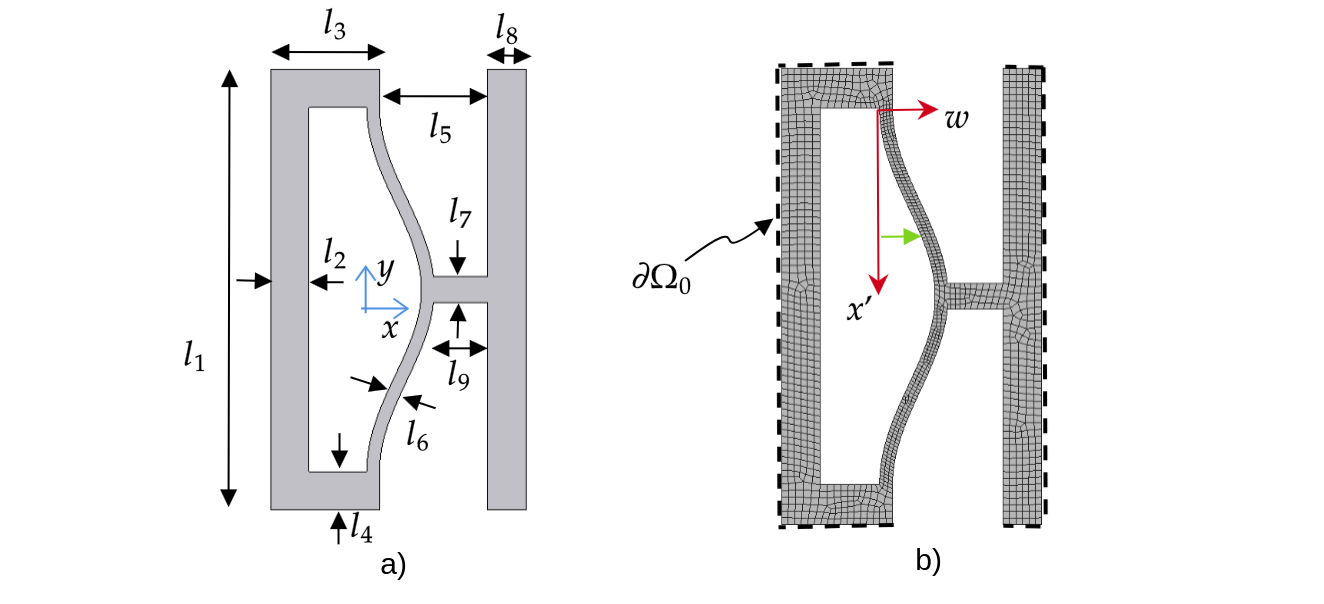
\includegraphics[width=0.8\textwidth]{FIGS/cell.png}
    \caption{Geometry and finite element discretization of the
    metamaterial unit cell (the geometry is based on the design proposed in Ref.~\cite{chen2025negative}).
    (a) Reference domain, with
    \(l_1=60.40~\mathrm{mm}\),
    \(l_2=l_4=l_8=5.20~\mathrm{mm}\),
    \(l_3=14.50~\mathrm{mm}\),
    \(l_5=14.90~\mathrm{mm}\),
    \(l_6=1.76~\mathrm{mm}\),
    \(l_7=3.50~\mathrm{mm}\), and
    \(l_9=7.49~\mathrm{mm}\).
    The centerline of the lower
    curved ligament is described in the local coordinates
    \((x',w)\) by
    \(w(x')=\frac{h}{2}
    [1-\cos(\pi x'/L)]\), \(0\leq x'\leq 2L\), where
    \(2L=l_1-2l_4=50.00~\mathrm{mm}\) is its projected span and
    \(h=l_5-l_9-l_6=5.65~\mathrm{mm}\) is its maximum transverse rise.
    (b) Finite element mesh; the dashed markers identify the external
    boundary \(\partial\Omega_0\), whose opposite sides are paired for
    the imposition of periodic boundary conditions.}
    \label{fig:cell_geometry}
\end{figure}
The  material is modeled as an isotropic compressible
Neo--Hookean solid under plane-strain conditions, with Young's modulus
\(E=1628~\mathrm{MPa}\) and Poisson's ratio \(\nu=0.4\). The domain is
discretized using \(\nel = 1315\) bilinear quadrilateral elements (average size $0.1~mm$) and \(1602\)
nodes; $\ngpel = 4$  Gauss points  are employed per element, giving a total of
\(\ngp=\nel \ngpel =  5260\) integration points.


The cell is deformed    exclusively through its external boundary $\partial \Omega_0$ via imposed displacements (thus
\(\Fext=\zero\) in Eq.~\refeq{eq:Rfe_definition}). Furthermore, the boundary term $\dBOUND$ in Eq.~\refeq{eq:dvecreconstruction} is assumed to be linear with the input parameter $\muvec$, i.e., $\dBOUND=\Umacro\muvec$,
  the columns of $\Umacro$ defininig the prescribed displacement patterns for unit variations of each component of $\muvec$. To give this   parametrization a concrete mechanical
interpretation, \(\Umacro\) is constructed from the periodic boundary
conditions of first-order computational homogenization\footnote{Lest this modeling choice be mistaken for an endorsement of
first-order homogenization for bistable media, we emphasize that it is
adopted here for simplicity rather than fidelity. Its kinematic content
is too limited to represent the full complexity of bistable
unit cells. Richer nonlinear multiscale formulations endowed with
micromorphic variables are more appropriate for that purpose; see,
e.g., Ref.~\cite{sperling2024comparative}.} at finite
strains; see, e.g., Ref.~\cite{miehe2003computational}. %Varying \(\muvec\) then amounts to solving the same unit-cell
%problem for many prescribed macroscopic deformation states, thereby
%defining the multi-query setting for which model reduction is intended.
  More specifically, the input parameters are identified with two   components (thus $\nmu = 2$) of the macroscopic displacement gradient $\Gmacro \in \RRn{2}{2}$:  the normal
component along the \(x\)-direction and the shear component, i.e.:
\begin{equation}
\label{eq:meta_macro_gradient}
    \muvec
    =
    \begin{bmatrix}
        \Gmacrox\\
        \Gmacroxy
    \end{bmatrix}.
\end{equation}
The transverse normal component is set to zero, and \(\Gmacro\) is assumed
symmetric, so that no macroscopic rigid-body rotation is prescribed; thus:
\begin{equation}
    \Gmacro(\muvec)
    =
    \begin{bmatrix}
        \Gmacrox  & \Gmacroxy\\
        \Gmacroxy & 0
    \end{bmatrix} =\begin{bmatrix}
        \mu_1  & \mu_2\\
        \mu_2 & 0
    \end{bmatrix}.
\end{equation}
Nonzero entries in $\Umacro$ appear only for slave boundary nodes   and   corner
nodes; such entries are determined by considering that,  for a node $\bm{X}=(X,Y)^T$, the   macroscopic contribution is defined   as $\bar{\bm{u}}(\bm{X})=\Gmacro \bm{X}$, which in the present
case yields $\bar{\bm{u}}(\bm{X})=( \mu_1 X+ \mu_2 Y,\,
\mu_2 X)^T$.

Consistently with this interpretation, \(\dred \in \Rn{\nL}\)  in
Eq.~\refeq{eq:dvecreconstruction} collects the degrees of freedom of
the interior nodes and the independent boundary nodes on the
designated master sides for imposing periodic conditions (here $\nL = 3018$). On the other hand, the lifting operator \(\Tlift\) in Eq.~\refeq{eq:dvecreconstruction} transfers the
periodic fluctuation displacements from the master sides to their
paired slave sides.


As customary in first-order computational homogenization, the output of
interest is the homogenized first Piola--Kirchhoff stress,
\begin{equation}
\label{eq:meta_homogenized_stress}
    \PKmacro
    =
    \frac{1}{|\Omega_0|}
    \int_{\Omega_0}\PKone\,d\Omega_0,
\end{equation}
which is a volumetric output \(\yOUT\) of the form introduced in
Eq.~\refeq{eq:generic_output_FE_quadrature}; hence,  $\rOUT = \PKone/|\Omega_0| $ and  \(\ncond=4\).

% The benchmark represents a multi-query problem in which the same
% microscopic boundary-value problem must be evaluated for many prescribed
% macroscopic deformation states. The objective is to replace these
% repeated FE solutions with a nonlinear-manifold reduced model that
% reconstructs the microscopic displacement field and evaluates
% \(\PKmacro\) through a sparse manifold-adaptive cubature rule.



\subsection{Training data}

% \input{Training1}
The training set \(\PmuTRAIN\) (see Eq.~\ref{eq:pmutrain})  is   restricted to a
two-dimensional rectangle, in order to keep the regression problem simple and to
allow a direct graphical inspection of the adaptive weights. The compression/stretching
component along the soft direction of the cell is varied in the interval
$ \Gmacrox \in [-0.42,\,0.42]$, whereas the shear component is varied in
$\Gmacroxy \in [-0.05,\,0.05]$. As illustrated in Fig.~\ref{fig:param_space}, the lower bound
\((\Gmacrox)_{\textrm{min}}=-0.42\) corresponds to the most compressed configuration before self-contact occurs\footnote{Our model does not include any
representation of self-contact; hence, extrapolation beyond this
compression level would be physically meaningless.}.    Although these cells are primarily intended to operate under compression,
the parameter domain is  kept symmetric, with
\((\Gmacrox)_{\textrm{max}} = 0.42\). The purpose is to test the reduced model in
a prediction regime in which input parameters of the same magnitude but
opposite sign generate outputs of markedly different magnitude (as shown
later, in Figure~\ref{fig:standard_HROM_stress}, the corresponding stress levels in the $x$ direction  may differ by up to a factor of
\(25\), since buckling of the curved ligaments leads to a substantially softer
response under compression).
\begin{figure}[!ht]
    \centering
    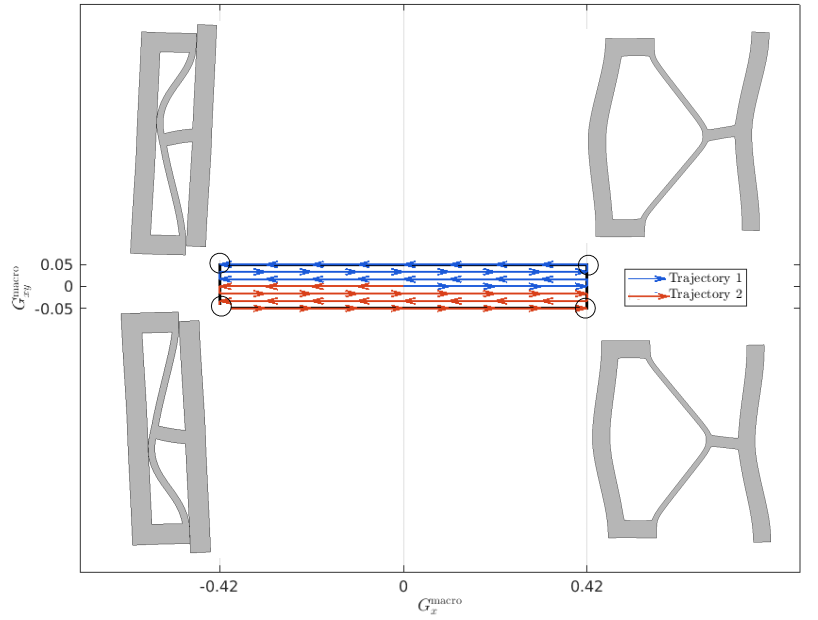
\includegraphics[width=0.85\textwidth]{FIGS/param_space.png}
    \caption{Training parameter domain and zig-zag trajectories used to
generate the FE displacement snapshots. The corner configurations
correspond to the extreme parameter values.}
    \label{fig:param_space}
\end{figure}

We sample the rectangular parameter domain   using a
Cartesian grid with \(230\) and \(20\) uniform intervals in the
\(\Gmacrox\)- and \(\Gmacroxy\)-directions, respectively. This gives
\(\nsnap=231\cdot21=4851\) distinct parameter states.  The FE simulations corresponding to each of these parameters is obtained by   traversing this grid along two continuous zig-zag
loading trajectories, covering the nonnegative and nonpositive shear
regions, respectively (see Fig.~\ref{fig:param_space}).




\subsection{Standard HROM  }
 \label{sec:meta_standard_hrom}


 %\input{sHROM}
 %\input{sHROM2}
 %\input{sHROM3}
 %\input{sHROM4}
We begin by assessing the
efficiency of the standard HROM. This
model is recovered as a particular case of the manifold HROM introduced
in Section~\ref{sec:decoderENCODER} by identifying, in the decoder
factorization of Eq.~\refeq{eq:decoder_tau_generic},  \(\qM\) with the standard reduced coordinates
\(\qrom\), and by taking \(\TAU(\qrom)=\qrom\). It then follows that
\(\JTAU=\ident\) in Eq.~\refeq{eq:JTAU} and
\(\PhiD=\PhiROM\) in Eq.~\refeq{eq:PhiD_tau_generic}.


 The accuracy and complexity of this model are governed solely by the
truncation tolerances $\tolSVDd$, for determining the displacement basis  \(\PhiROM\), see Eq.~\ref{eq:PhiROM_truncation}, and   \(\tolSVD\), for the integrand matrix \(\Ucub\), see Eq.~\refeq{eq:Ucub_definition}.  Both bases are computed using the
Sequential Randomized SVD   of
Ref.~\cite{hernandez2024cecm}, briefly introduced in
Section~\ref{sec:fixed_weight_cubature}.\footnote{For
\(\rROM=52\), the integrand matrix \(\Agen\) has \(5260\) rows, one per
candidate Gauss point, and
\((\rROM+\nOUT)\nsnap=(52+4)\times4851=271656\) columns. Its explicit
storage in double precision requires approximately \(11.4\,\mathrm{GB}\),
excluding factorization costs. The SRSVD is therefore particularly useful
under memory limitations, as it processes the state-wise blocks
\(\Agen_j\) sequentially without assembling the complete matrix. \label{footnote:size}}
We then performed a systematic tolerance study and selected the least
expensive configuration for which the normalized maximum error in the
homogenized stress remained below \(0.1\%\) over the complete training
set. The study revealed that this criterion requires \(\tolSVDd=10^{-6}\), yielding a basis matrix $\PhiROM$ with
\(\rROM=52\) modes, and  \(\tolSVD=10^{-4}\), which results in an
ECM rule with \(1340\) Gauss points. For illustration,
Fig.~\ref{fig:standard_HROM_results}(a) shows the \(671\) finite elements
containing these points.

The tight displacement truncation tolerance
\(\tolSVDd=10^{-6}\) required to meet the accuracy criterion for the stresses reflects the previously mentioned
markedly different scales of the tensile and compressive responses shown
in Fig.~\ref{fig:standard_HROM_results}(b). Indeed, modes associated with small
singular values contribute little to the snapshot energy, yet are necessary to  capture local details related to
 internal buckling mechanisms governing the low-stress compressive
branch.

 \begin{figure}[!ht]
    \centering
    \begin{subfigure}[t]{0.2\textwidth}
        \centering
        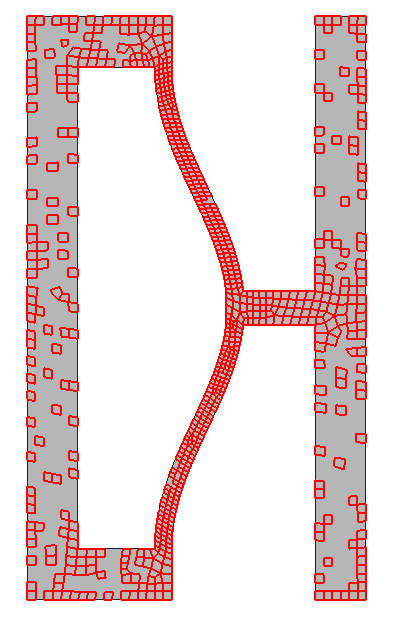
\includegraphics[width=\textwidth]{FIGS/elems1.png}
        \caption{Elements containing the selected Gauss points.}
        \label{fig:standard_HROM_support}
    \end{subfigure}
    \hfill
    \begin{subfigure}[t]{0.7\textwidth}
        \centering
        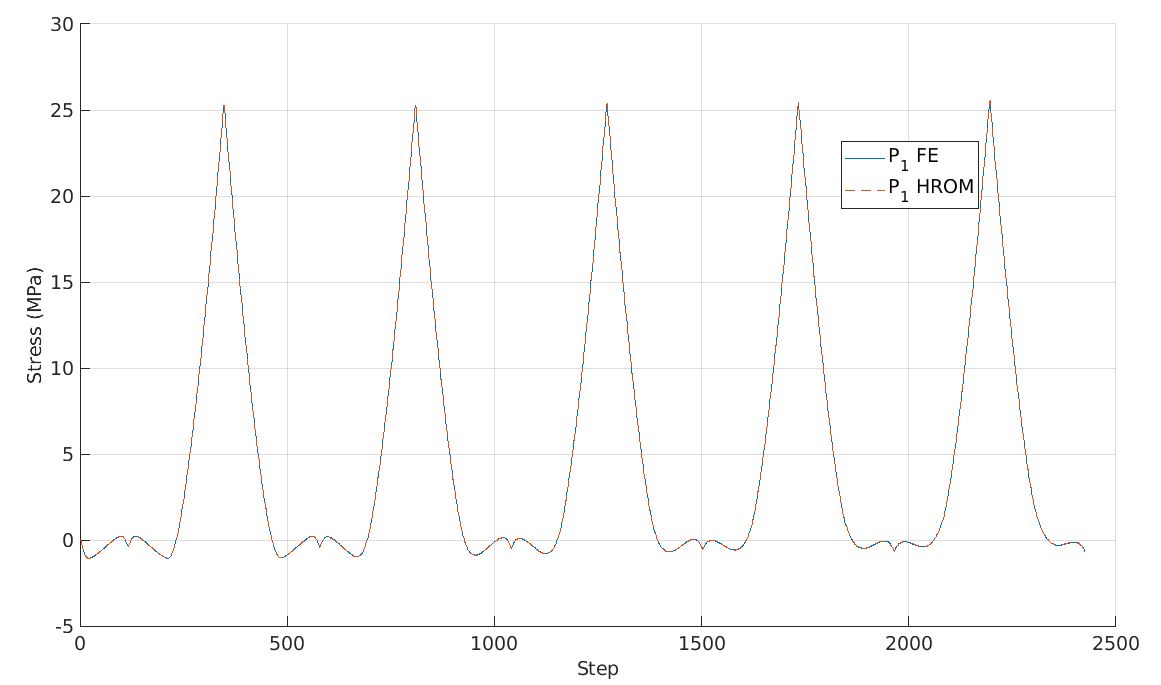
\includegraphics[width=\textwidth]{FIGS/case37.png}
        \caption{Homogenized \(P_x\) response.}
        \label{fig:standard_HROM_stress}
    \end{subfigure}
    \caption{Standard-HROM results for
    \(\tolSVDd=10^{-6}\) and \(\tolSVD=10^{-4}\).
    (a) The ECM rule comprises \(1340\) Gauss points distributed over
    \(671\) finite elements. (b) FE and standard-HROM homogenized PK1
    stress histories along the second trajectory in
    Fig.~\ref{fig:param_space}; the HROM uses \(\rROM=52\) displacement
    modes.}
    \label{fig:standard_HROM_results}
\end{figure}

In summary, even though the problem is governed by  \(\nmu=2\) parameters,    $\rROM=52$ linear displacement modes are required
to reproduce the nonlinear response with the desired accuracy. This  illustrates the poor
linear compressibility of the problem under study. The
limitation is even more apparent at the hyperreduction level, where the
fixed ECM rule retains  1340 of the original $\ngp=5260$ integration points (approximately 25\%).




\subsection{Manifold HROM}
\subsubsection{Identification of latent coordinates}
\label{sec:meta_manifold_representation}

 %\input{Decoder1}
 %\input{Decoder2}
%\input{Decoder3}
 The poor linear compressibility observed above motivates replacing the
linear reduced representation with the nonlinear-manifold approximation
of Eq.~\refeq{eq:decoder_master_slave}, introduced in
Section~\ref{sec:fact}. We first address the identification of the
latent coordinates. As established in Eq.~\refeq{eq:qMdefq}, these are
obtained from the modal coefficients through
\(\qM=\Tm\qrom\); the task here is therefore to determine the
transformation matrix \(\Tm\) by exploiting the particular structure of
the present benchmark.


The  problem under consideration is static (no inertial effects) and the material response is hyperelastic (no path dependence). It can be argued that, under such circumnstances,   the displacement
state $\dred$ admits a single-valued parametrization in terms of prescribed
  input \(\muvec\). This implies that the dimension of the solution manifold is   equal to the dimension of the input parameter space ($\rD=\nmu=2$), and, furthermore, that   there is a one-to-one mapping between input parameters and the desired latent coordinates:
  \begin{equation}
   \qM = \varphiM(\muvec).
  \end{equation}
  For the present benchmark, \(\Tm\) is determined by requiring that the above map     approximate the identity
map over the training set. In view of Eq.~\refeq{eq:qMdefq}, this
amounts to making $
    \qM(\muvec_j)-\muvec_j
    =
    \Tm\qrom(\muvec_j)-\muvec_j
$ as small as possible for every training input \(\muvec_j\) ($j=1,2 \ldots \nsnap$). Collecting
the modal coefficients and the corresponding input parameters into
\begin{equation}
\label{eq:meta_coordinate_matrices}
    \Qrom
    \defeq
    \PhiROM^T\Dsnap,
    \qquad
    \Mtrain
    \defeq
    \begin{bmatrix}
        \muvec_1 & \muvec_2 & \cdots & \muvec_{\nsnap}
    \end{bmatrix},
\end{equation}
(here, \(\Dsnap\) is the displacement snapshot matrix introduced in
Eq.~\refeq{eq:manifold_snapshot_matrix}.), the matrix \(\Tm\) is accordingly obtained from the least-squares problem
\begin{equation}
\label{eq:least_squares_master_coordinates}
    \Tm
    =
    \arg\min_{\widetilde{\Tm}}
    \left\|
        \widetilde{\Tm}\Qrom-\Mtrain
    \right\|_F^2.
\end{equation}
  Assuming $\Qrom$ has full rank, the  solution of Problem \refeq{eq:least_squares_master_coordinates} is unique and  given by
\begin{equation}
\label{eq:least_squares_master_coordinates_solution}
    \Tm
    =
    \Mtrain\Qrom^\dagger
\end{equation}
where \(\Qrom^\dagger\) denotes the Moore--Penrose pseudoinverse.

The relative value of the least-squares residual at the optimum for the problem under consideration is
\begin{equation}
\label{eq:latent_parameter_residual}
    \frac{
        \left\|\Tm\Qrom-\Mtrain\right\|_F
    }{
        \left\|\Mtrain\right\|_F
    }
    =
    3.09\cdot10^{-7}.
\end{equation}
Thus, to numerical accuracy, the latent coordinates associated with the
training states can be identified with the   input parameters:
\begin{equation}
\label{eq:input_aligned_coordinates}
    \qM\approx\muvec.
\end{equation}

\begin{remark}
\label{remark:noiterations}
This identification has an important consequence for the online stage
of the present benchmark. Because \(\qM\) is obtained directly from the
prescribed input \(\muvec\), the reduced equilibrium equations
\refeq{eq:MAW_ROM_equilibrium} need not be solved to determine the
latent state. The decoder can instead be evaluated directly at
\(\qM\approx\muvec\). Hyperreduction through the proposed adaptive
cubature rule is therefore required only for evaluating the homogenized
stresses (the equilibrium-residual integrands need not be included in
the cubature training problem).
\end{remark}

\subsubsection{Nonlinear closure}
\label{sec:nonlinearclosure}
%\input{Decoder4}
Once \(\Tm\) has been determined, the master basis \(\PhiM\) and the
scaling matrix \(\Am\) follow from the SVD of
\(\PhiROM\Tm^T\) introduced in Section~\ref{sec:fact}, together with
Eq.~\refeq{eq:Am_definition}. The slave basis \(\PhiS\) is subsequently
obtained from the orthogonality conditions in Eq.~\refeq{eq:orto}. For
the present problem, this decomposition yields the $\rD = 2$ master modes whose deformed shapes are depicted in Figures \ref{fig:master_mode_1} and \ref{fig:master_mode_2}, and
\(\rROM-\rD=50\) slave modes (the deformed shapes of some of these modes are in turn shown in Figures \ref{fig:slave_mode_1} to \ref{fig:slave_mode_4} ),  with
\begin{equation}
\label{eq:meta_Am}
    \Am
    =
    10^{-1}
    \begin{bmatrix}
        -3.9962  &  0.21588\\
        -0.34716 & -6.4264
    \end{bmatrix}.
\end{equation}




\begin{figure}[H]
    \centering

    \begin{subfigure}{0.23\textwidth}
        \centering
        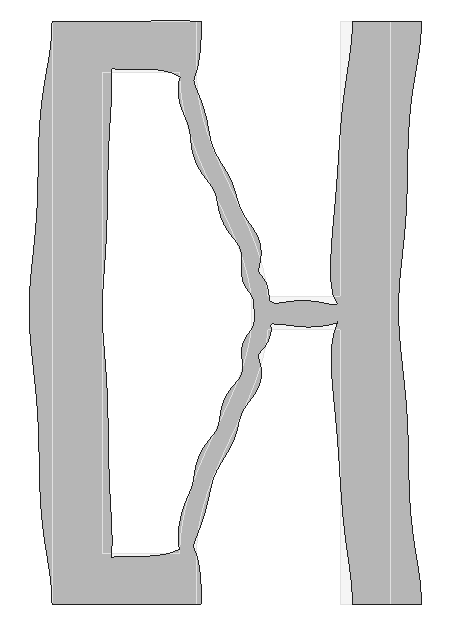
\includegraphics[width=\textwidth]{FIGS/m1m.png}
        \caption{Master mode \({\PhiM}_1\).}
                \label{fig:master_mode_1}
    \end{subfigure}
    \hspace{0.05\textwidth}
    \begin{subfigure}{0.23\textwidth}
        \centering
        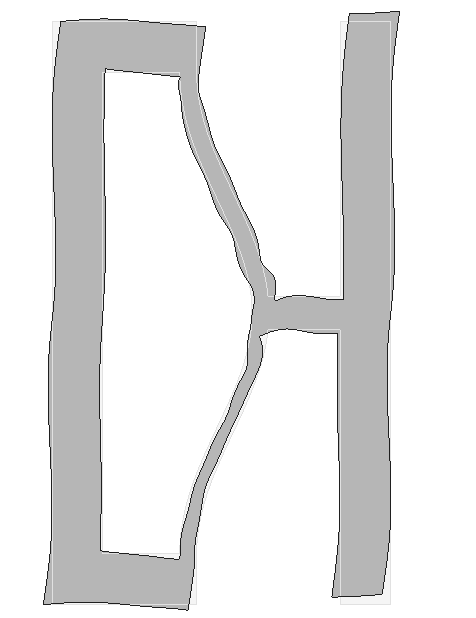
\includegraphics[width=\textwidth]{FIGS/m2m.png}
        \caption{Master mode \({\PhiM}_2\).}
                \label{fig:master_mode_2}
    \end{subfigure}

    \vspace{0.5em}

    \begin{subfigure}{0.23\textwidth}
        \centering
        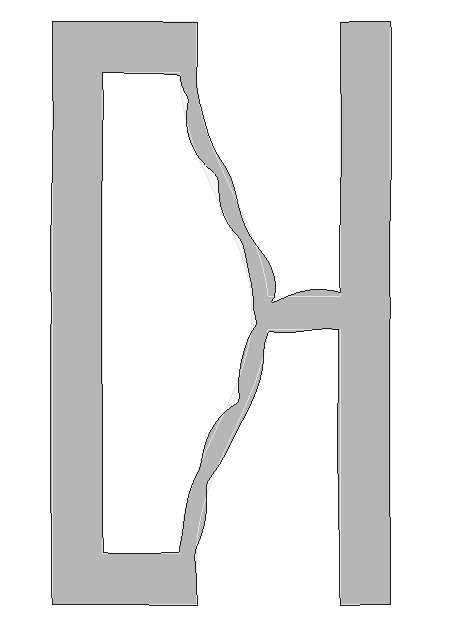
\includegraphics[width=\textwidth]{FIGS/slv1.png}
        \caption{Slave mode \({\PhiS}_1\).}
          \label{fig:slave_mode_1}
    \end{subfigure}
    \begin{subfigure}{0.23\textwidth}
        \centering
        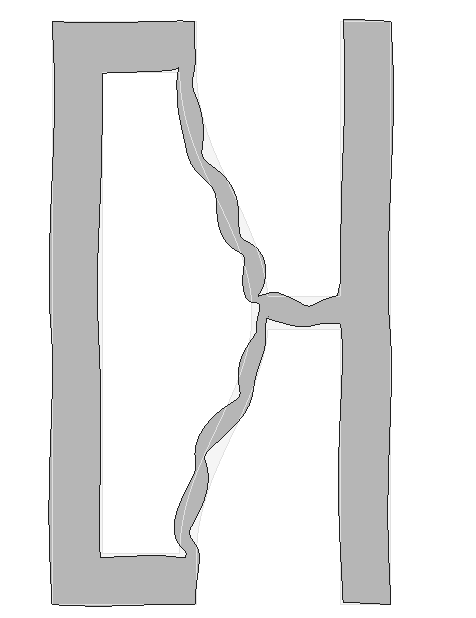
\includegraphics[width=\textwidth]{FIGS/slv5.png}
        \caption{Slave mode \({\PhiS}_6\).}
         \label{fig:slave_mode_2}
    \end{subfigure}
    \begin{subfigure}{0.23\textwidth}
        \centering
        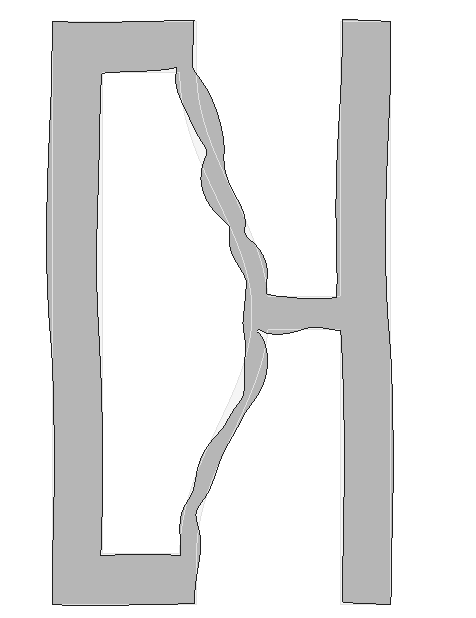
\includegraphics[width=\textwidth]{FIGS/slv13.png}
        \caption{Slave mode \({\PhiS}_{13}\).}
        \label{fig:slave_mode_3}
    \end{subfigure}
    \begin{subfigure}{0.2\textwidth}
        \centering
        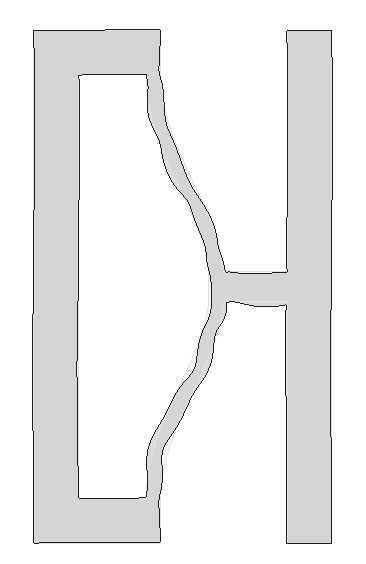
\includegraphics[width=\textwidth]{FIGS/slv44.png}
        \caption{Slave mode \({\PhiS}_{44}\).}
        \label{fig:slave_mode_4}
    \end{subfigure}

    \caption{Deformed shapes of the $\rD = 2$ master modes $\PhiM$ and four of the  $\rROM-\rD = 50$    slave modes $\PhiS$.  The modal vectors,
    originally defined on the independent degrees of freedom, are extended
    to the complete nodal space through the lifting operator \(\Tlift\)
    for visualization (see Eq.~\refeq{eq:dvecreconstruction}).}
    \label{fig:master_slave_modes_manifold}
\end{figure}

   It remains to identify the nonlinear closure mapping the
\(\rD=2\) latent coordinates onto the
\(\rROM-\rD=50\) slave coordinates,
\(\qS\approx\Nslave(\qM)\). To this end, we employ anisotropic
Gaussian radial basis functions (RBFs) augmented with polynomial
terms (quadratic). The regression coefficients are determined through
standard-form Tikhonov-regularized least squares, using the identity
regularization matrix ( see
Refs.~\cite{poggio1990networks,wendland2005scattered}).

Only a subset of the available snapshot pairs is retained as RBF
centers. A structured subsampling frequency of \([3,1]\) is used:
every third sample is retained along the first latent direction
(compression/extension), whereas all samples are retained along the
second direction (shear). This results in \(1540\) centers out of $\nsnap =4851$ data points. The
remaining states are employed to assess the accuracy of the closure away
from the retained centers.

The characteristic lengths of the anisotropic Gaussian kernels are set to
\(\ell_1=3.3013\cdot10^{-2}\) and
\(\ell_2=1.5789\cdot10^{-2}\), and the Tikhonov regularization
parameter  to \(\lambda_{\mathrm{RBF}}=10^{-10}\). With these
settings, the relative reconstruction error is
\(4.30\cdot10^{-6}\) at the retained centers and
\(1.03\cdot10^{-4}\) over the complete dataset.

Figure~\ref{fig:meta_slave_closure} shows the resulting mappings for
four representative slave coordinates. The reconstructed surfaces are
smooth and single-valued over the sampled latent domain, while the
black markers indicate the retained RBF centers.


\begin{figure}[H]
    \centering

    \begin{subfigure}{0.45\textwidth}
        \centering
        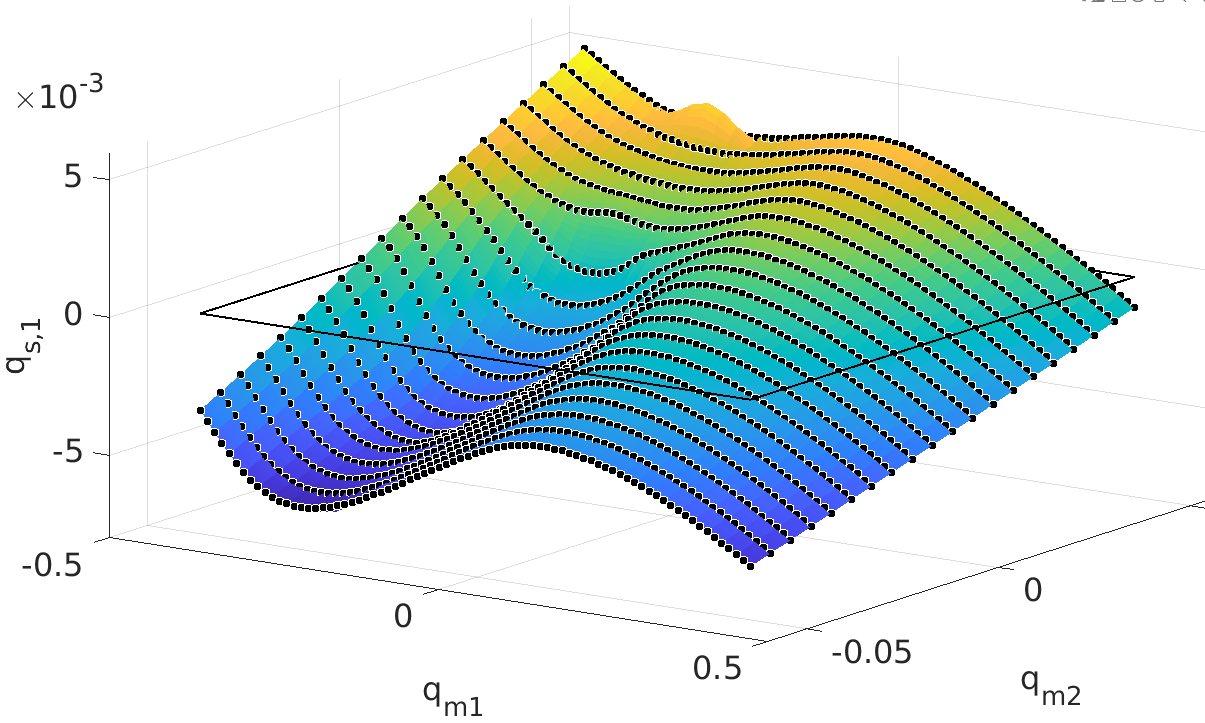
\includegraphics[width=\textwidth]{FIGS/rbf1.png}
        \caption{Slave amplitude \((\qS)_1\).}
        \label{fig:RBF_slave_surface_1}
    \end{subfigure}
    \hfill
    \begin{subfigure}{0.45\textwidth}
        \centering
        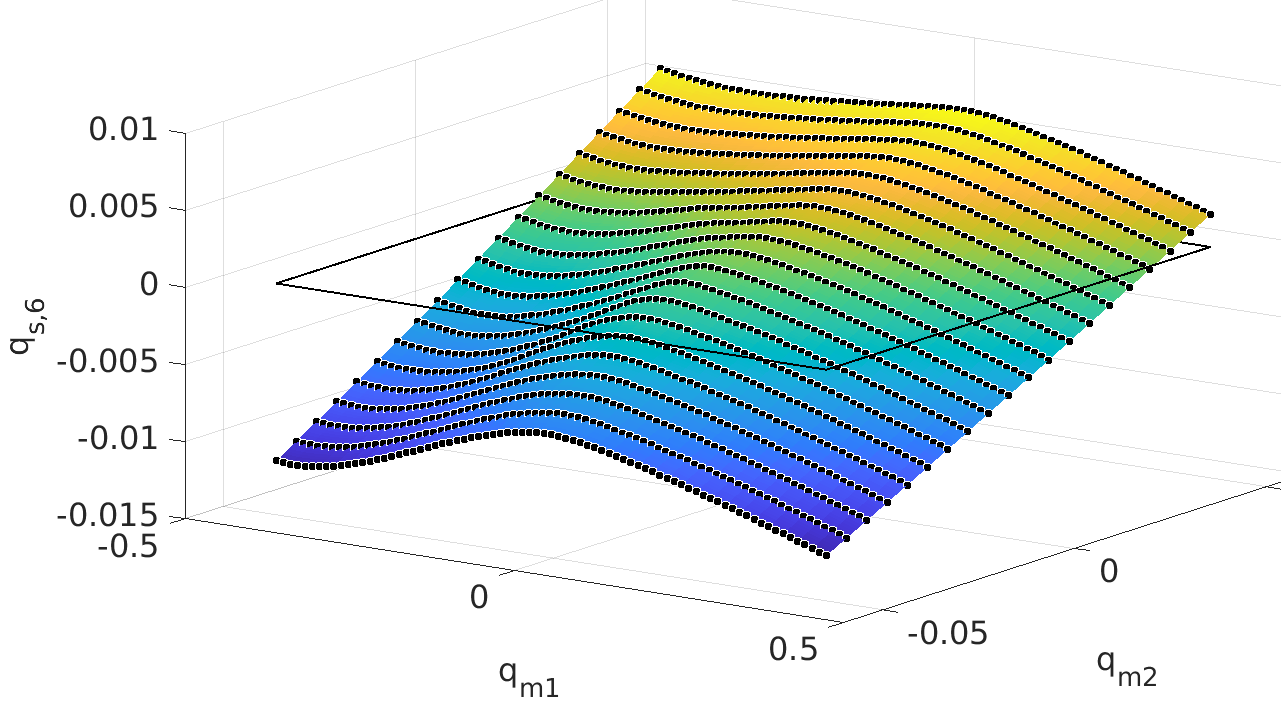
\includegraphics[width=\textwidth]{FIGS/rbf6.png}
        \caption{Slave amplitude \((\qS)_6\).}
        \label{fig:RBF_slave_surface_6}
    \end{subfigure}

    \vspace{0.5em}

    \begin{subfigure}{0.45\textwidth}
        \centering
        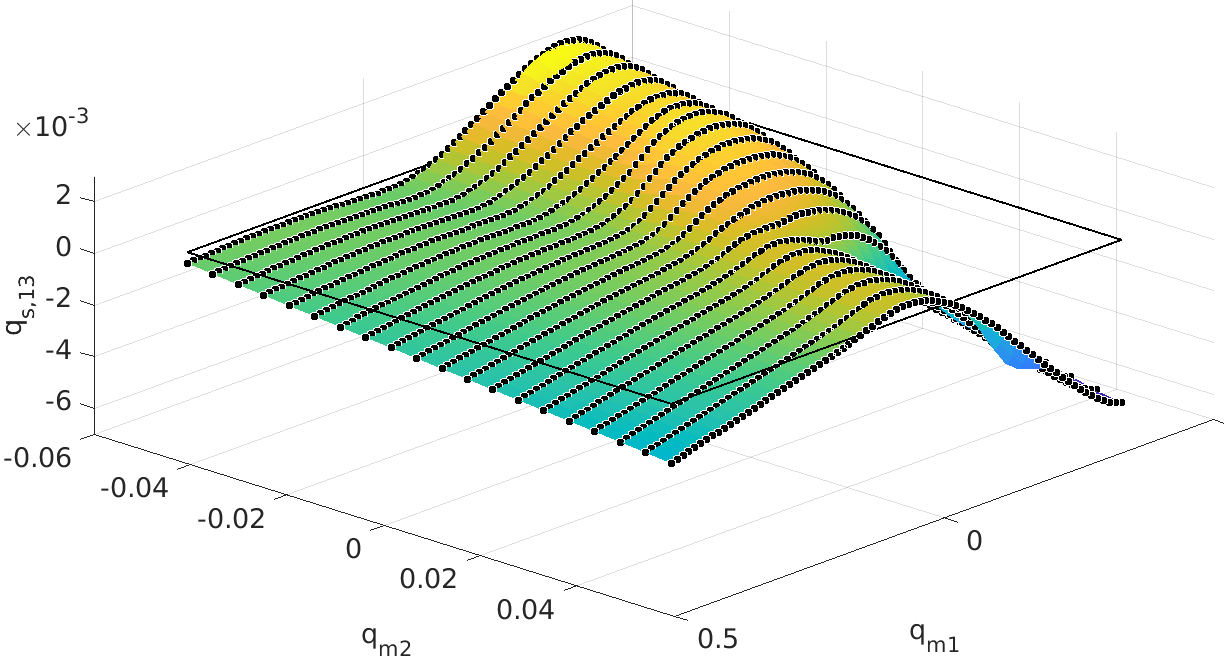
\includegraphics[width=\textwidth]{FIGS/rbf13.png}
        \caption{Slave amplitude \((\qS)_{13}\).}
        \label{fig:RBF_slave_surface_13}
    \end{subfigure}
    \hfill
    \begin{subfigure}{0.45\textwidth}
        \centering
        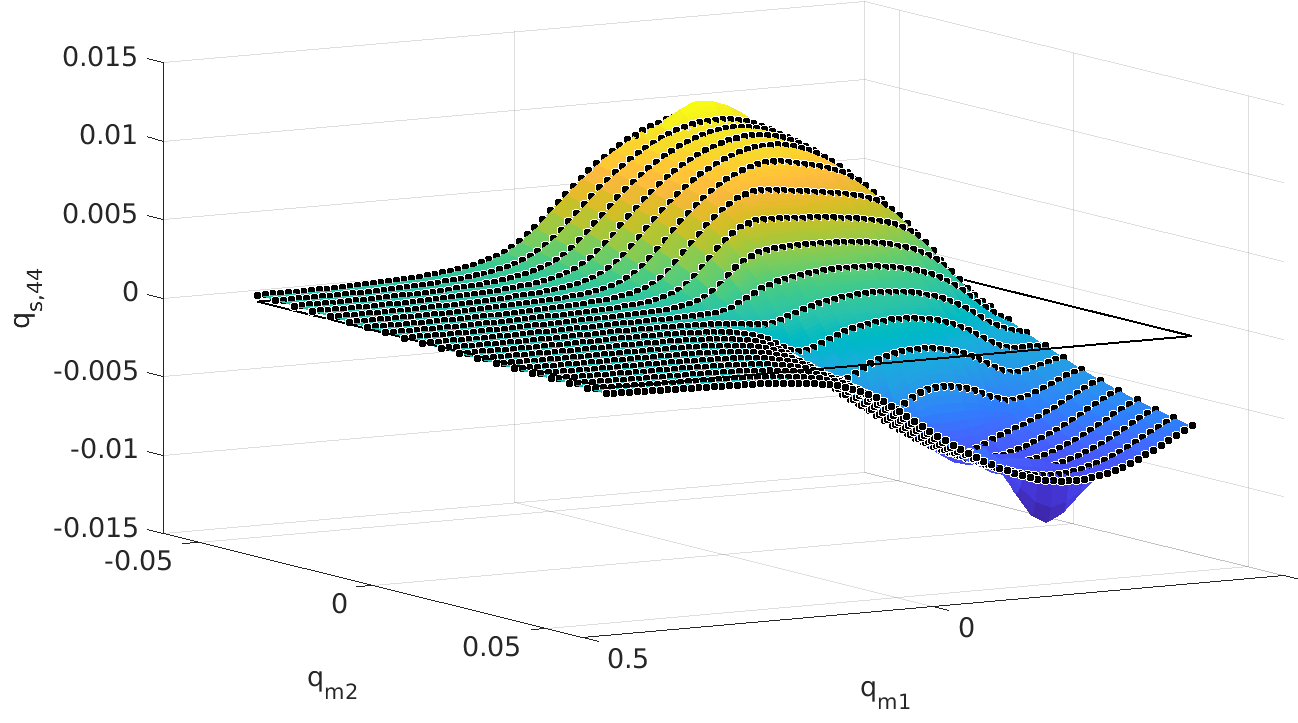
\includegraphics[width=\textwidth]{FIGS/rbf44.png}
        \caption{Slave amplitude \((\qS)_{44}\).}
        \label{fig:RBF_slave_surface_44}
    \end{subfigure}

    \caption{RBF reconstructions of four representative slave amplitudes
    over the two-dimensional latent space. The black markers denote the
    retained RBF centers.}
    \label{fig:meta_slave_closure}
\end{figure}


\subsubsection{Fixed-weight ECM}
\label{sec:fixedECM1}
With the manifold coordinates and the slave closure in place, we next
construct the fixed-weight ECM rule, discussed in Section~\ref{sec:fixedweight_cubature}. As noted in Remark~\ref{remark:noiterations},  the latent state is prescribed directly by the macroscopic
input, and no reduced equilibrium problem needs
to be solved for the evaluation of the homogenized response. We
therefore adopt the output-only case described after
Eq.~\refeq{eq:approxGEN} in Section~\ref{sec:fixedweight_cubature}  and construct the cubature rule exclusively
for the homogenized stress in Eq.~\refeq{eq:meta_homogenized_stress}, that is:  $\rGENg{g}= {\PKone_g}/{|\Omega_0|}$ ($g=1,2 \ldots \ngp$), which implies that there are  $\ncond = 1+ \nstress = 5$ integration conditions per state. The same \(\nM=1540\) retained latent states used for the RBF closure described previously in Section \ref{sec:nonlinearclosure} are employed to assemble the output-integrand matrix $\Agen$ defined in Eq.~\ref{eq:AgenDEF}; hence\footnote{This matrix is markedly smaller than its standard-HROM
counterpart, which contains
\((\rROM+\nOUT)\nsnap=271656\) columns; see
Footnote~\ref{footnote:size} in
Section~\ref{sec:meta_standard_hrom}. The number of scalar fields
processed by the SRSVD is therefore reduced by a factor of
approximately \(44\), substantially alleviating the memory demands
associated with the construction of the ECM basis. }  $\Agen \in
    \mathbb{R}^{\ngp\times(\nstress\nM)}     =     \mathbb{R}^{5260\times6160}$. Using the SRSVD with \(\tolSVD=10^{-4}\) to compress \(\Agen\), and
augmenting the resulting basis with the volume constraint in
Eq.~\refeq{eq:ECM_volume_constraint}, the ECM yields a fixed rule with
\(\mInit=54\) Gauss points distributed over \(48\) finite elements.

Table~\ref{tab:online_fixed_manifold} compares  the accuracy of the fixed-weight manifold
approximation with those of the standard ROM and HROM. Here,
\(\errdisp\) denotes the relative Frobenius error in the independent
displacement histories, whereas \(\errPK\) is the corresponding
relative Frobenius error in the homogenized PK1 stress histories, in
both cases using the FE solution as reference. The errors are computed
separately over each complete loading trajectory and then averaged over
the two trajectories.

\begin{table}[!ht]
\centering
\caption{Online complexity (in terms of number of master/slave coordinates, and number of integration points  ) and accuracy  (relative Frobenius norms in displacements, $\errdisp$ and stresses $\errPK$)  of the fixed-weight manifold
HROM, together with the standard standard ROM and HROM.   }
\label{tab:online_fixed_manifold}
\begin{tabular}{lccccc}
\toprule
Model
& Master coords.
& Slave coords.
& Integ. points
& \(\errdisp\)
& \(\errPK\) \\
\midrule
ROM, full Gauss rule
& \(52\) & \(0\) & \(5260\)
& \(2.52\cdot10^{-6}\)
& \(5.05\cdot10^{-5}\) \\
HROM, ECM
& \(52\) & \(0\) & \(1340\)
& \(1.85\cdot10^{-5}\)
& \(7.13\cdot10^{-5}\) \\
M-HROM, fixed ECM
& \(2\) & \(50\) & \(54\)
& \(7.87\cdot10^{-5}\)
& \(2.98\cdot10^{-4}\) \\
\bottomrule
\end{tabular}
\end{table}

 Table~\ref{tab:online_fixed_manifold} shows that the manifold HROM
increases the homogenized-stress error by a factor of approximately four
relative to the standard HROM. This loss of accuracy is due to the    subsampling and subsequent regression (recall that  the
error is evaluated over all \(\nsnap=4851\) states, whereas the closure
is fitted using only \(\nM=1540\) retained centers). The resulting
accuracy--compression trade-off is nevertheless strongly favorable: the number of
independent coordinates decreases from \(\rROM = 52\) to \(\rD=2\), and the
number of integration points from \(1340\) to \(\mInit = 54\). Interestingly,
the corresponding compression ratios are almost identical, namely
\(26\) and approximately \(25\), respectively. Moreover, the direct
identification of the master coordinates with the input eliminates the
reduced nonlinear equilibrium solve.


\subsection{Manifold-adaptive weight ECM }



The preceding fixed-weight manifold HROM completes the kinematic
compression, but its cubature rule remains global: the same
\(\mInit=54\) weights must represent the homogenized-stress integrands
over the entire latent domain. The final stage of the compression
process is therefore to exploit the manifold structure also at the
cubature level, by allowing the weights to vary with the latent state.
Following the formulation of Section~\ref{sec:MAWECM}, the fixed-weight
ECM rule provides the initial candidate support \(\ZD\) and the feasible
initial weight vector \(\omegaInit\). The greedy strategy of
Section~\ref{sec:Greedy} then progressively removes integration points
and redistributes the remaining weights over the sampled manifold while
preserving the local exactness and positivity conditions.

In the present output-only setting, the state-dependent integrands are
the $\nstress =4$ components of the   PK1 stress entering the
homogenized response. At each retained latent state, these four
integration conditions are supplemented with the invariant volume
constraint. The local systems in
Eq.~\refeq{eq:constraintsLOCAL} therefore contain $\ncond = \nstress + 1$ independent
conditions, which also establishes a lower bound of $\mLower = \ncond = 5$ points for any
positive adaptive rule.

The same \(\nM=1540\) states retained as RBF centers for the decoder are used as the
nodes of the latent graph \(\Glat\). Here, the numerical identification
\(\qM\approx\muvec\), together with the Cartesian sampling of the input
parameter domain (see Figure \ref{fig:standard_HROM_results}), makes the graph construction immediate: the retained
latent states inherit the connectivity of the structured parameter
grid. Adjacent states are connected to define an auxiliary
quadrilateral mesh in latent space, and the graph operator \(\KGs \in \RRn{1540}{1540}\) is
assembled from the standard finite element discretization of an
isotropic Laplacian using bilinear shape functions, consistently with
the graph-regularized redistribution described in
Section~\ref{sec:Greedy}.

\subsubsection{Influence of the fixed-weight initialization and pruning
efficiency}
\label{sec:infl_fw_ini}

We first assess the reduction achieved by the MAW--ECM pruning strategy
of Algorithm~\ref{alg:MAW_global_pruning}, and its sensitivity to the
fixed-weight initialization. The regularity of the resulting adaptive
weight fields, their regression over the latent domain, and the
associated online accuracy are examined subsequently.

Four initial cubature rules are considered, obtained with
\[
\tolSVDfixed\in
\left\{10^{-4},10^{-5},10^{-6},10^{-7}\right\}
\]
in the truncation of the training integrand matrix \(\Agen\). The case
\(\tolSVDfixed=10^{-4}\) is precisely the \(\mInit=54\)-point rule
assessed in Table~\ref{tab:online_fixed_manifold}. The other three rules
are introduced here solely to determine whether the final adaptive
support and the pruning efficiency depend materially on the size and
accuracy of the fixed-weight initialization.

The graph-regularization parameter and the number of candidate trials
are held fixed throughout the study at
\(\alphaG=10^4\), appearing in
Algorithm~\ref{alg:prune_step_optionB}, and
\(\ntry=5\), appearing in
Algorithm~\ref{alg:graph_candidate_sweep}. These values were selected
after preliminary experimentation as a compromise between regularity of
the adaptive weight fields and computational efficiency during pruning.






\begin{table}[ht!]
\centering
\caption{Influence of the fixed-weight initialization on the MAW--ECM pruning process for different values of the   SVD truncation tolerance $\tolSVDfixed$ for the integrand matrix $\Agen$.  Here, $\mInit$ denotes the number of points of the resulting initial fixed-weight ECM rule, and $\nomega$ the final number of points after pruning. \emph{First-stage limit} denotes the minimum number of points reached before positivity enforcement and graph regularization are activated in Algorithm~\ref{alg:prune_step_optionB}. \emph{Total time} corresponds to the wall-clock time of Algorithm~\ref{alg:MAW_global_pruning}, whereas \emph{Full-regularized time} denotes the wall-clock time obtained when regularization is applied during all pruning steps.    }
\label{tab:maw_pruning_summary}
\begin{tabular}{cccccc}
\hline
$\tolSVDfixed$ & $\mInit$ & First-stage limit &   $\nomega$ & Total time  (s) & Full-regularized time (s) \\
\hline
$10^{-4}$ & $54$  & $20$ & $10$ & $50.0$ & $  1172.0$ \\
$10^{-5}$ & $87$  & $18$ & $9$  & $44.0$ & $  7682.0$  \\
$10^{-6}$ & $135$ & $18$ & $10$ & $58.0$ & --- \\
$10^{-7}$ & $187$ & $19$ & $10$ & $89.0$ & --- \\
\hline
\end{tabular}
\end{table}


 Table~\ref{tab:maw_pruning_summary} summarizes the results obtained
with the four initial cubature rules. The most striking observation is
the weak dependence of the final adaptive rule on the initialization.
As the fixed-weight tolerance becomes more stringent, the size of the
initial rule increases markedly, from \(\mInit=54\) to
\(\mInit=187\). Nevertheless, the pruning algorithm consistently
reduces these rules to either \(\nomega=9\) or \(\nomega=10\)
integration points. Thus, the final support appears to be nearly
independent of the initial one. Moreover, the resulting adaptive rules
contain only about twice the theoretical lower bound,
\(\mLower=5\).

%
 An equally important observation concerns the behavior of the first pruning stage, namely the stage in which positivity enforcement is not explicitly activated.  As can be gleaned from the third column of Table~\ref{tab:maw_pruning_summary}, independently of the initial number of points, this stage systematically reduces the number of points  down to approximately $18$--$20$   before positivity violations begin to appear (Line~\ref{alg1:enforceREQUIRE} of Algorithm~\ref{alg:prune_step_optionB}). Thus, not only the final number of cubature points, but also the number of points at which positivity violations appear, seems to be essentially independent of the initial number of points.

 This behavior has a direct impact on computational efficiency (see last two columns of Table~\ref{tab:maw_pruning_summary}). For instance,   increasing the initial support from $54$ to $87$ points produces   no increase in wall-clock time (which remains below one minute in both cases\footnote{All computations
were performed in MATLAB on a Linux laptop,
equipped with a 13th-generation Intel Core i9-13900H processor and
16~GiB of RAM.}). This confirms the rationale behind Algorithm~\ref{alg:prune_step_optionB} and the proposed two-stage strategy: the computational cost is governed primarily not by the initial number of candidate points, but by the number of pruning iterations requiring activation of the graph-regularized positivity-enforcement stage.

In order to quantify the computational gains introduced by the proposed two-stage strategy, we compare the performance of the algorithm against a modified version in which the first pruning stage is artificially suppressed. This is achieved by temporarily disabling, for testing purposes, the conditional skip in Line~\ref{alg1:success3} of Algorithm~\ref{alg:prune_step_optionB} (namely, the line stating ``Successful pruning step, no need for regularization''). Under this modification, graph regularization is enforced throughout the entire pruning process, leading to a dramatic increase in computational cost.  In particular, the case $\mInit = 54$ increases from   $50$ seconds to approximately $20$ minutes, whereas the case $\mInit = 87$ increases from   $44$ seconds to more than two hours.

  \PROMPT{\input{PromptMeta1}}

 %
 %\input{MAW_ECM2}
%\subsection{Numerical results}

%\subsection{Discussion}

\subsubsection{Adaptive cubature rule and weight-field regression}
\label{subsec:num_char_adaptive_weights}

% \begin{figure}[!ht]
% \centering
% \subfloat[Initial fixed-weight cubature rule ($\mInit=54$).]{
% 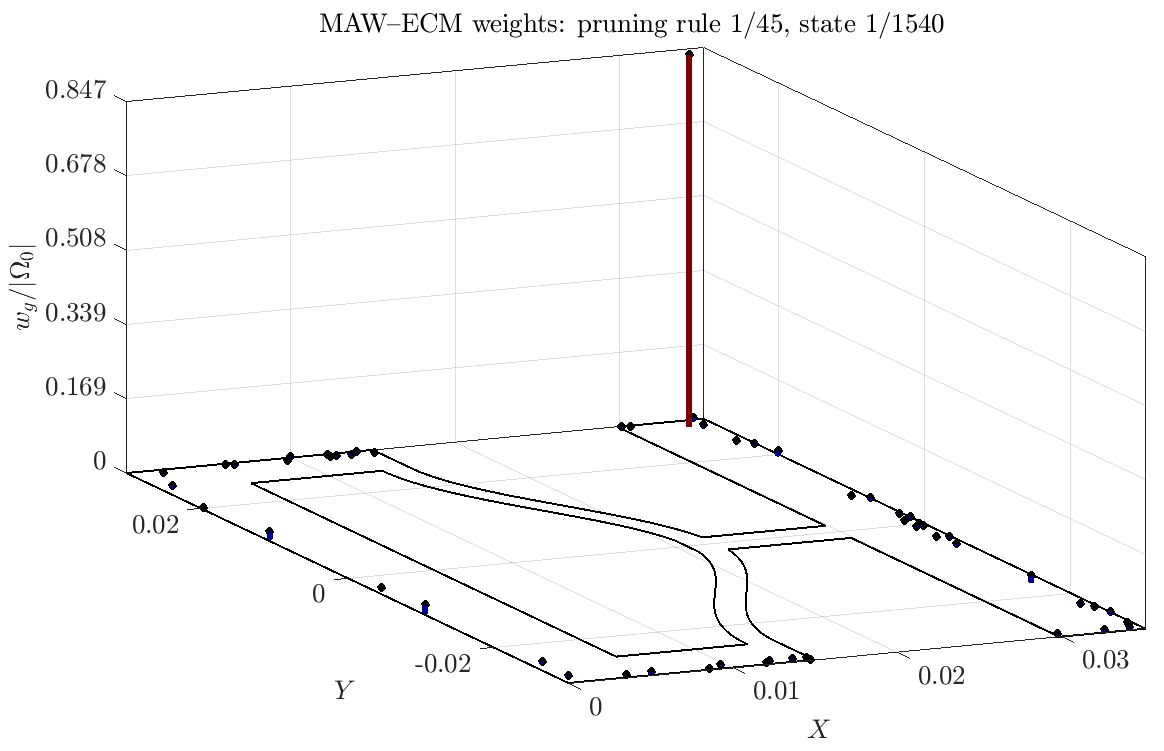
\includegraphics[width=0.48\textwidth]{FIGS/ECM54.png}}
% \hfill
% \subfloat[Final adaptive cubature rule ($\nomega=10$).]{
% 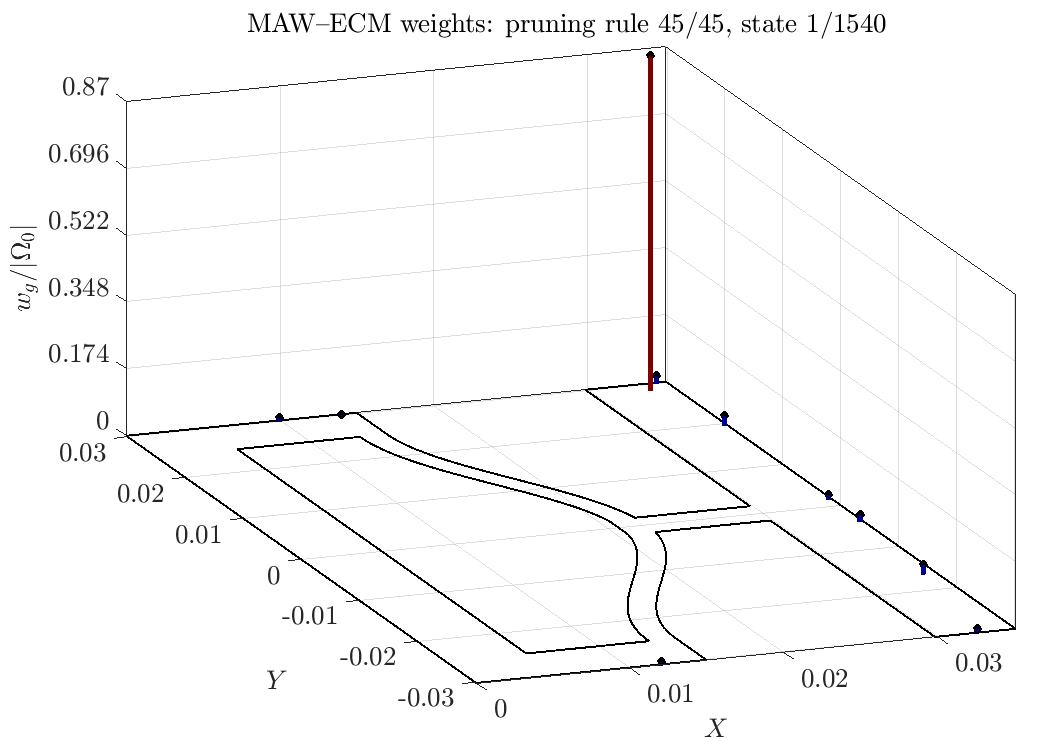
\includegraphics[width=0.48\textwidth]{FIGS/ECM_MAW_10.png}}
% \caption{Spatial location and associated weights of the integration points before and after the adaptive pruning process. The left figure shows the initial fixed-weight cubature rule ($\mInit=54$), whereas the right figure shows the final adaptive rule ($\nomega=10$) evaluated at   the origin of the latent manifold ($\qMone=\qMtwo=0$). Heights are proportional to the corresponding cubature weights. }
% \label{fig:ecm54_vs_maw10}
% \end{figure}
\begin{figure}[!ht]
\centering

\subfloat[Initial fixed-weight cubature rule ($\mInit=54$).]{
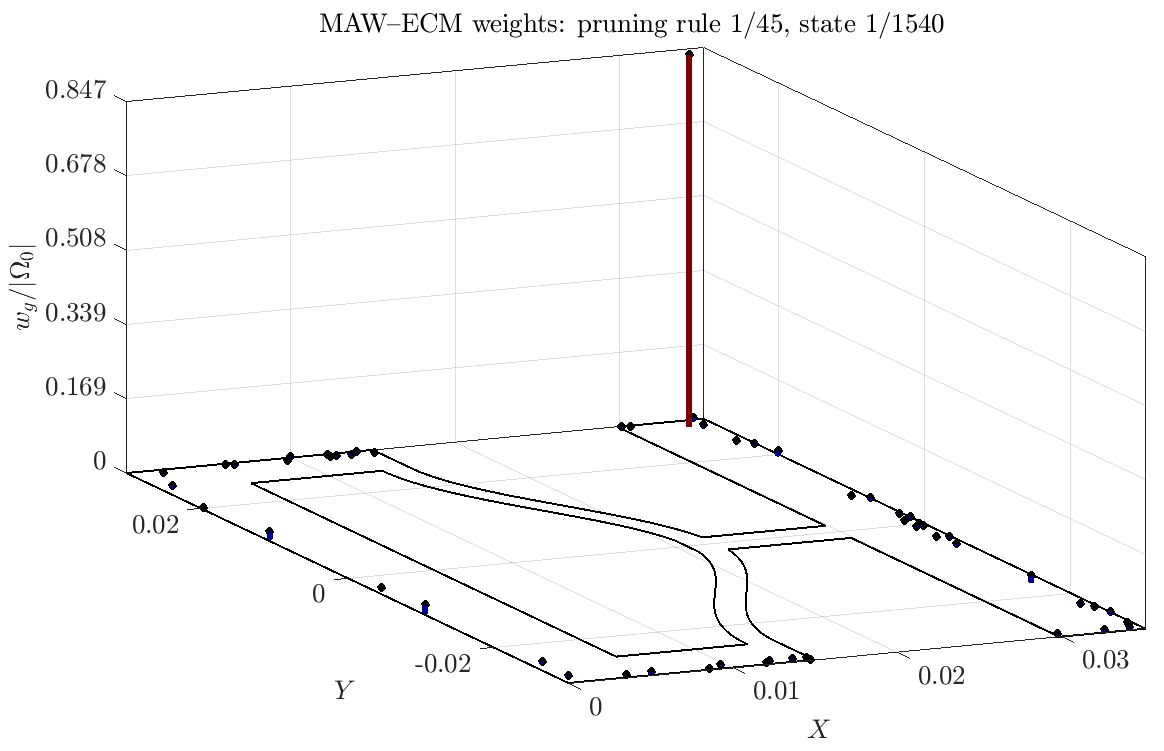
\includegraphics[width=0.48\textwidth]{FIGS/ECM54.png} \label{fig:ecm54a}}
\hfill
\subfloat[Final adaptive cubature rule for $\qMone = \qMtwo = 0$ ($\nomega=10$).]{
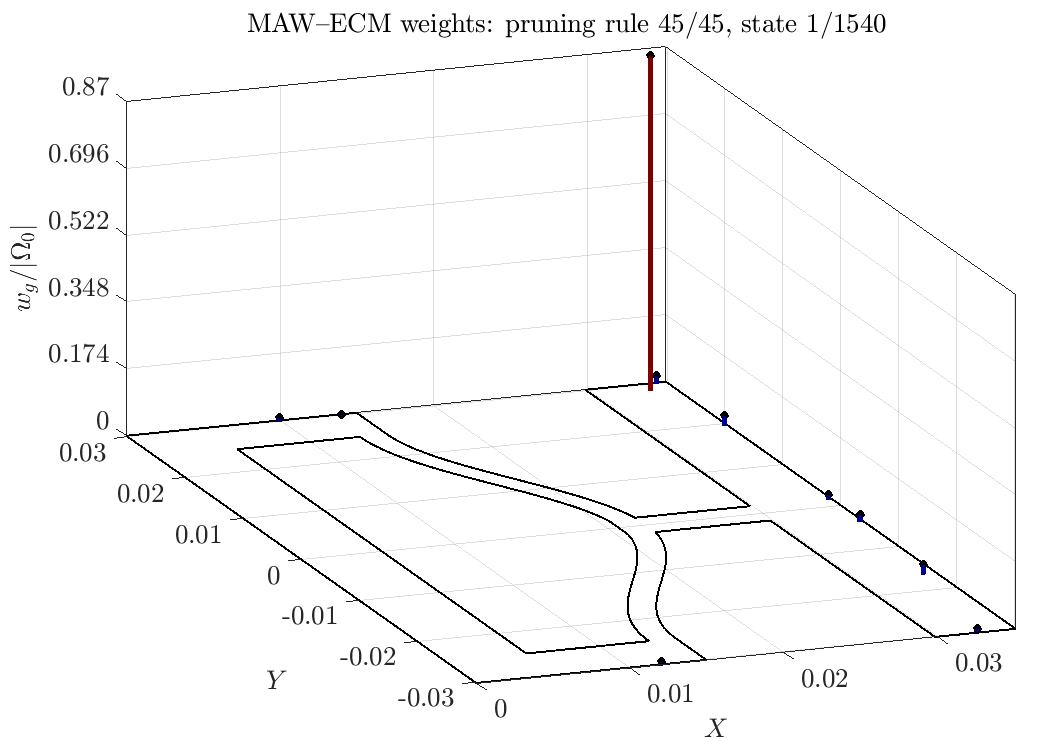
\includegraphics[width=0.48\textwidth]{FIGS/ECM_MAW_10.png}  \label{fig:ecm10a}}

\vspace{0.3cm}

\subfloat[Elements containing the $\mInit = 54$ integration points of the initial fixed-weight rule.]{
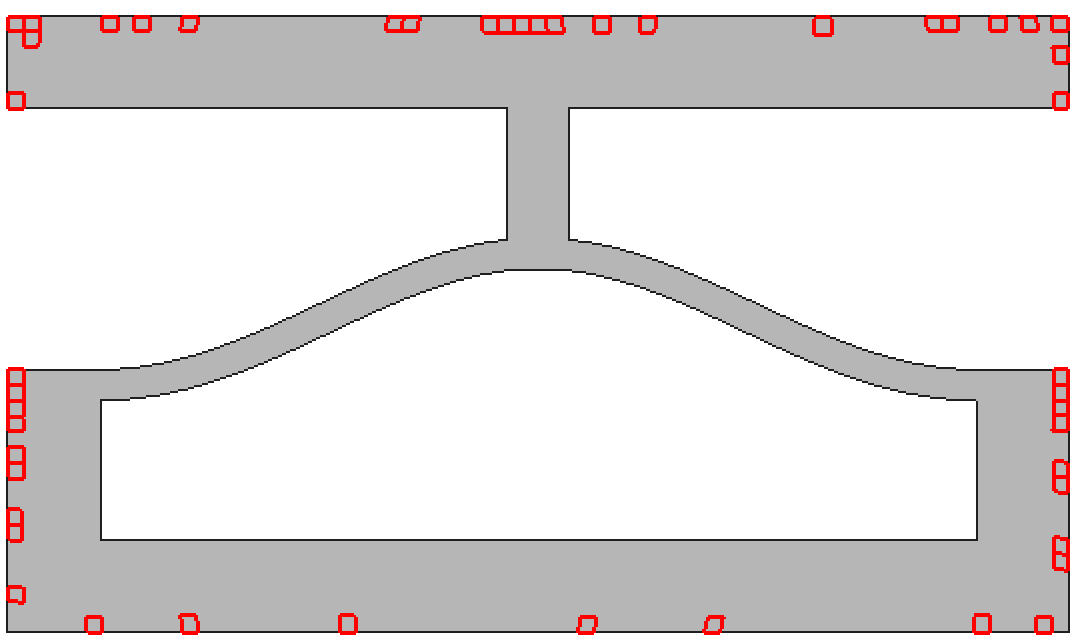
\includegraphics[width=0.4\textwidth]{FIGS/p54b.png} \label{fig:ecm54b}}
\hfill
\subfloat[Subset of elements containing the $\nomega  = 10$ integration points of the final adaptive rule.]{
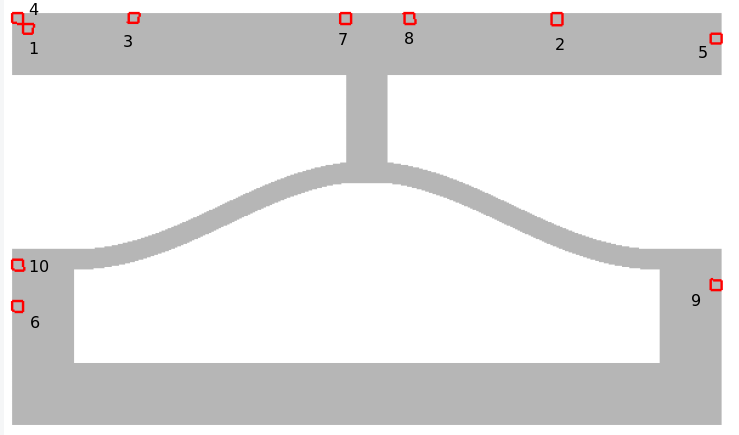
\includegraphics[width=0.4\textwidth]{FIGS/MAWecm10elem.png}  \label{fig:ecm10b}}

\caption{
Comparison between the initial fixed-weight manifold ECM rule and the final adaptive cubature rule obtained after pruning. The upper row shows the associated cubature weights, whereas the lower row identifies the elements containing the selected Gauss points.  The adaptive rule shown in the right column corresponds to latent state $\qMone=\qMtwo=0$. Heights in the upper row are proportional to the corresponding cubature weights.
}
\label{fig:ecm54_vs_maw10}
\end{figure}


Having quantified the level of reduction afforded by MAW--ECM, we next examine the structure of the resulting adaptive rule in greater detail. In particular, we focus on the case $\mInit=54$, and analyze both the spatial distribution of the retained integration points and the associated distribution of weights.
Figure~\ref{fig:ecm54_vs_maw10} compares the initial fixed-weight rule   with the final adaptive rule containing $\nomega=10$ points (  for the particular state $\qMone=0$ and $\qMtwo=0$). The upper row displays the spatial location of the selected integration points and their associated cubature weights, whereas the lower row identifies the finite elements containing such points. Notice that the initial rule in Fig.~\ref{fig:ecm54a} is already highly non-uniform: one of the $54$ integration points carries approximately $85\%$ of the total volume. As discussed in Ref.~\cite{hernandez2024cecm}, this lack of uniformity is a characteristic feature of ECM-type cubature rules, reflecting the greedy, sparsity-promoting nature of the algorithm (which prioritizes error reduction over weight uniformity). It can be seen in Fig.~\ref{fig:ecm10a} that the adaptive pruning process preserves this dominant point (labelled as point~1), with its relative weight   increasing from $85\%$ to $87\%$ in the final rule.



%
% Another noteworthy feature concerns the location of the retained points. The point with the highest weight   belongs to an interior element, whereas all remaining points lie on elements adjacent to the interface boundaries. Interestingly, no point is retained on the boundary $X=0$, while five points (labelled ${2,3,4,7,8}$ in Fig.~\ref{fig:ecm10b}), belong to elements adjacent to the opposite face  $X=X_{\max}$.
%
% \begin{remark}
%  Recall that the quantity of interest is the homogenized PK1 stress, which, as pointed out in Section \ref{subsec:homogenized_PK1}, is recovered from the reaction forces acting on the interface boundaries (hence the   concentration of integration points within elements adjacent to such boundaries in the initial cubature rule).  From this perspective, the absence of integration points near the boundary $X=0$ in the final rule is   striking.  It  suggests  that the stress information carried by these points is somehow dependent  of that contained in the remaining support, specially those on the opposite side $X=X_{max}$. The MAW--ECM algorithm appears to detect indirectly these latent dependencies ( that  may originate from equilibrium, periodicity, and symmetry considerations), and encode them in the  variability of the adaptive weights of the retained  points.  In this regard, the resulting mechanism bears a certain resemblance to the master--slave relations employed in Section~\ref{subsec:manifold_identification_cell}: in both cases, information that initially appears distributed across many degrees of freedom/integration points is ultimately represented through a reduced set of independent quantities. The essential difference is that, here, the dependencies are  not explicitly constructed, but emerge naturally from the pruning process itself.
%  \end{remark}
%

 Once the support of the adaptive cubature rule has been identified, the next step consists of constructing continuous approximations of the associated adaptive weight fields, $\omegag{g}=\omegag{g}(\qM)$, $g=1,\ldots,\nomega$. Here, we use the same  anisotropic RBFs employed for the decoder, but with constant polynomial correction,   Tikhonov regularization parameter $\lambda=10^{-10}$ and characteristic length scales $\ellRBF_1 = 2.2\times10^{-2}$ and $\ellRBF_2 = 1.053\times10^{-2}$. Figure~\ref{fig:weights_alpha1e4_rbf} shows the resulting weight fields (normalized by the volume $|\Omega_0|$), together with the sampled manifold states (black dots).

\begin{figure}[!ht]
\centering
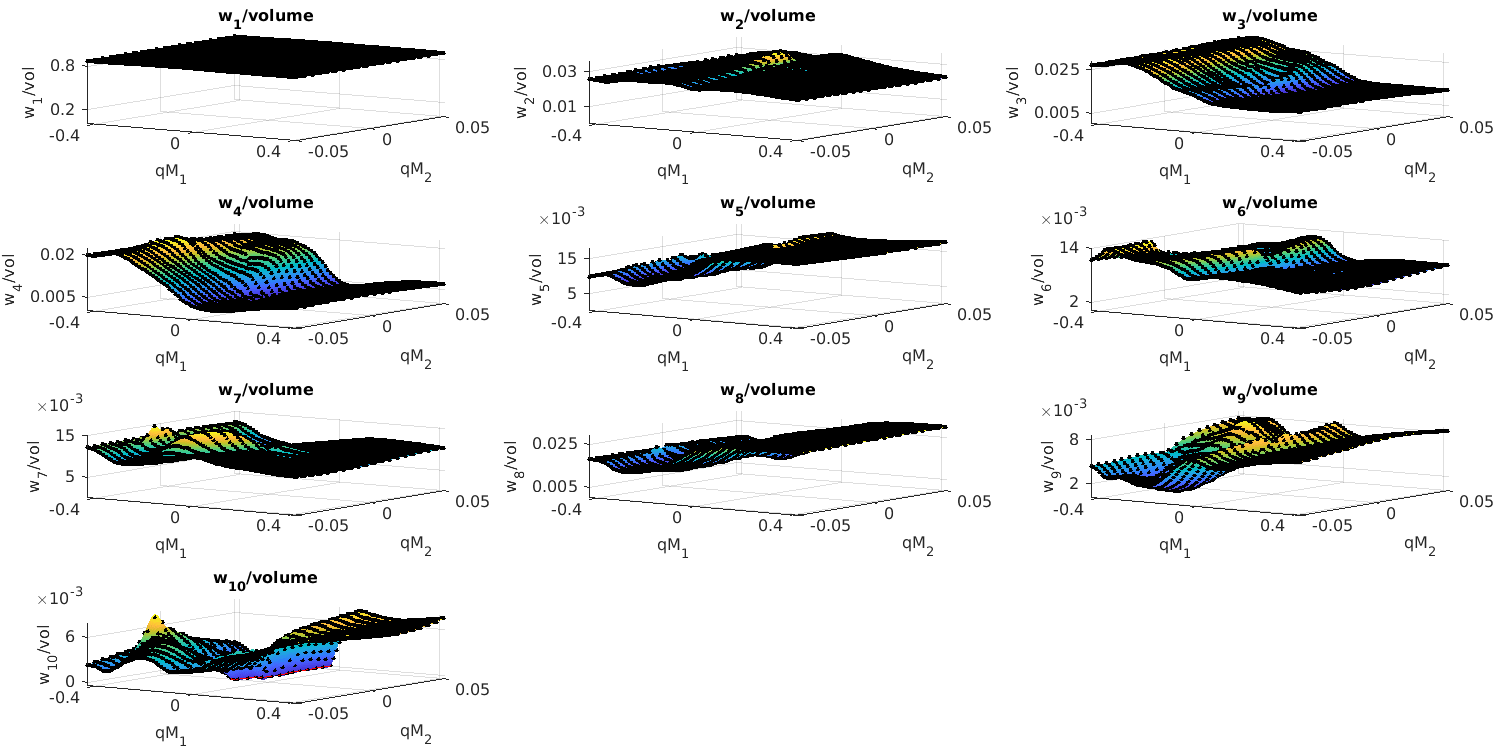
\includegraphics[width=\textwidth]{FIGS/weights_alpha1e4_RBF.png}
\caption{RBF reconstruction of the ten adaptive weight fields $\omegag{g}=\omegag{g}(\qM)$, $g=1,\ldots,\nomega$. Black dots denote the sampled manifold states used by the adaptive cubature procedure. The spatial location of the integration point associated with each weight field is shown in Fig.~\ref{fig:ecm10b}.}
\label{fig:weights_alpha1e4_rbf}
\end{figure}

The first weight field, $\omegag{1}$  remains nearly constant throughout the latent manifold and accounts for more than $87\%$ of the total volume. This observation further reinforces the interpretation of this point as primarily responsible for enforcing the volume-preservation constraint. The nontrivial variations are therefore concentrated in the remaining nine weight fields. Their average magnitude ranges from approximately $3.0\%$ of the total volume for $\omegag{2}$ down to only $0.05\%$ for $\omegag{10}$. Furthermore, the amplitude of the oscillations tends to increase as the average value of the corresponding weight decreases. Their average magnitude ranges from approximately $3.0\%$ of the total volume for $\omegag{2}$ down to only $0.05\%$ for $\omegag{10}$. At the same time, the spatial structure of the corresponding fields becomes progressively richer as their average magnitude decreases.  Nevertheless, all weight fields remain smooth functions of the latent coordinates, with no evidence of abrupt localized variations.  The RBF reconstruction yields a relative interpolation error of $3.89\cdot10^{-9}$ over the complete dataset.


\begin{figure}[!ht]
\centering
\subfloat[$\eta = 0.25 $]{
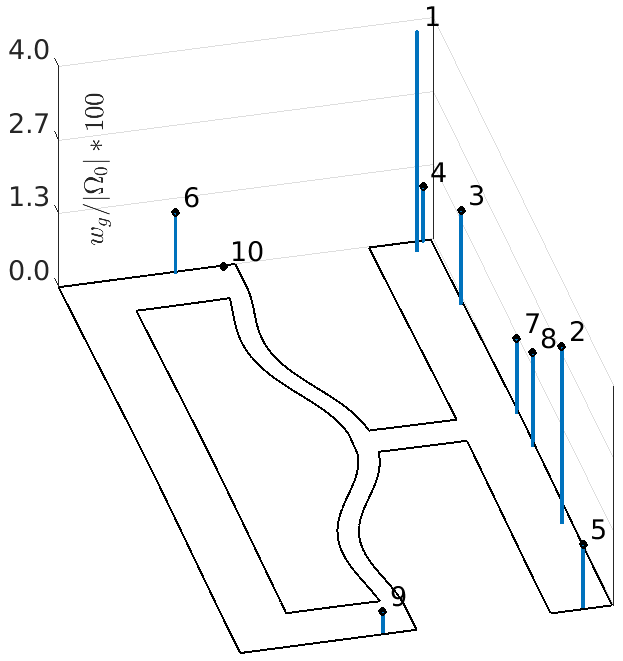
\includegraphics[width=0.24\textwidth]{FIGS/d25.png}}
\hfill
\subfloat[$\eta = 0.5 $]{
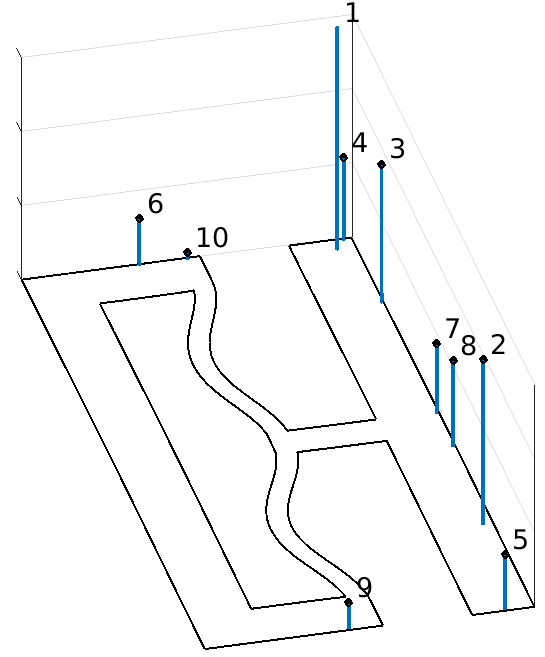
\includegraphics[width=0.23\textwidth]{FIGS/d50n.png}}
\hfill
\subfloat[$\eta = 0.75 $]{
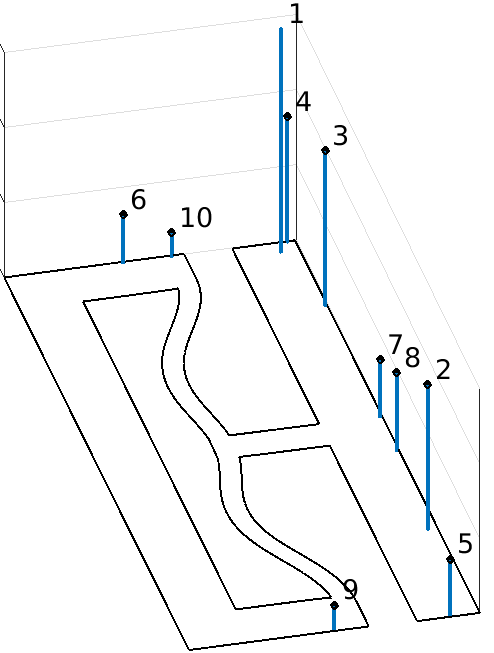
\includegraphics[width=0.21\textwidth]{FIGS/d75.png}}
\hfill
\subfloat[$\eta = 1.0 $]{
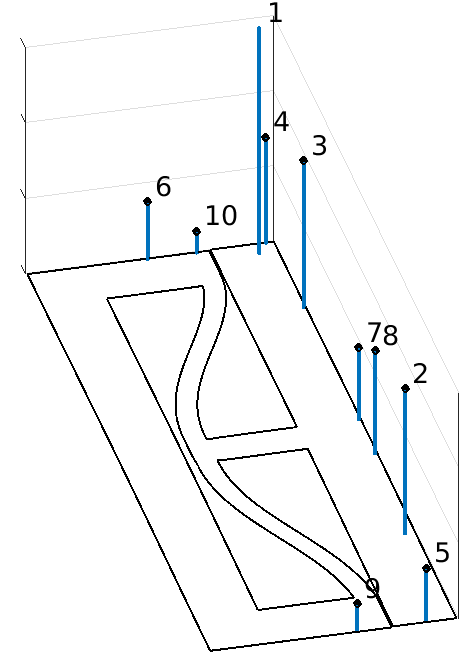
\includegraphics[width=0.21\textwidth]{FIGS/d100.png}}
\caption{Evolution of the adaptive cubature weights along a purely compressive loading path ($\qMtwo=\Gmacroxy=0$, $\qMone=\Gmacrox<0$). The quantity $\eta=\eta(\qMone)$ denotes the compression level ($\eta = 0$ for the undeformed configuration, and $\eta = 1$ for maximum compression). Each subfigure shows the deformed configuration of the unit cell together with the location of the $\nomega=10$ integration points and their associated weights, which evolve according to the regressed fields shown in Fig.~\ref{fig:weights_alpha1e4_rbf}. The height of each bar represents the percentage of the total volume carried by the corresponding integration point.  To make the redistribution among the smaller weights visible, the plotted height is truncated at $4\%$ of the total volume.  Consequently, the dominant weight $\omegag{1}$ is displayed only partially; its actual value is approximately $88.37\%$, $87.83\%$, $87.21\%$, and $86.99\%$ for $\eta=0.25$, $0.5$, $0.75$, and $1.0$, respectively.}
\label{fig:adaptive_weights_compression_path}
\end{figure}



An alternative way of visualizing the   weight variability is to exploit the fact that the the latent coordinates are approximately equal to the input macro-gradients ($\qMone\approx\Gmacrox$ and $\qMtwo\approx\Gmacroxy$). Thus, the adaptive weights can be interpreted directly as deformation-dependent quadrature weights.   Figure~\ref{fig:adaptive_weights_compression_path}
shows this interpretation along a purely compressive path, with
$\Gmacroxy=0$ and
$\Gmacrox<0$.  The deformed configuration of the unit cell is displayed together with the corresponding adaptive cubature weights.



\subsubsection{Effect of graph regularization}





Let us now qualitatively examine the effect of the graph regularization parameter $\alphaG$ on the smoothness of the resulting weight fields.  To this end, Fig.~\ref{fig:w3_alpha_comparison} compares the sampled values of the third weight field for $\alphaG=10^{4}$ (the same field previously shown in Fig.~\ref{fig:weights_alpha1e4_rbf}) and for $\alphaG=0$, i.e., in the absence of regularization. The benefits of the regularization are  evident: for $\alphaG=0$, the sampled values clearly exhibit stronger local fluctuations and a less coherent evolution over the latent manifold.

\begin{figure}[!ht]
\centering
\subfloat[$\alphaG=0$.]{
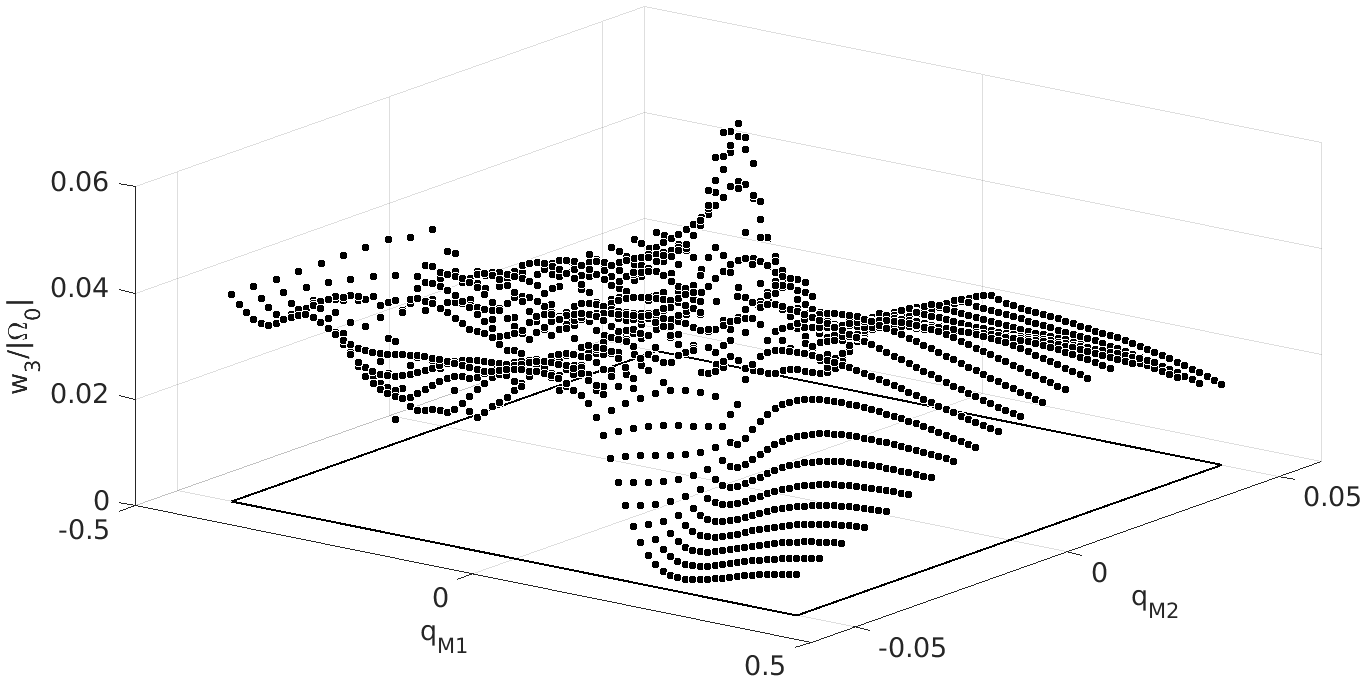
\includegraphics[width=0.48\textwidth]{FIGS/w3_alpha0.png} \label{fig:nor}}
\hfill
\subfloat[$\alphaG=10^{4}$.]{
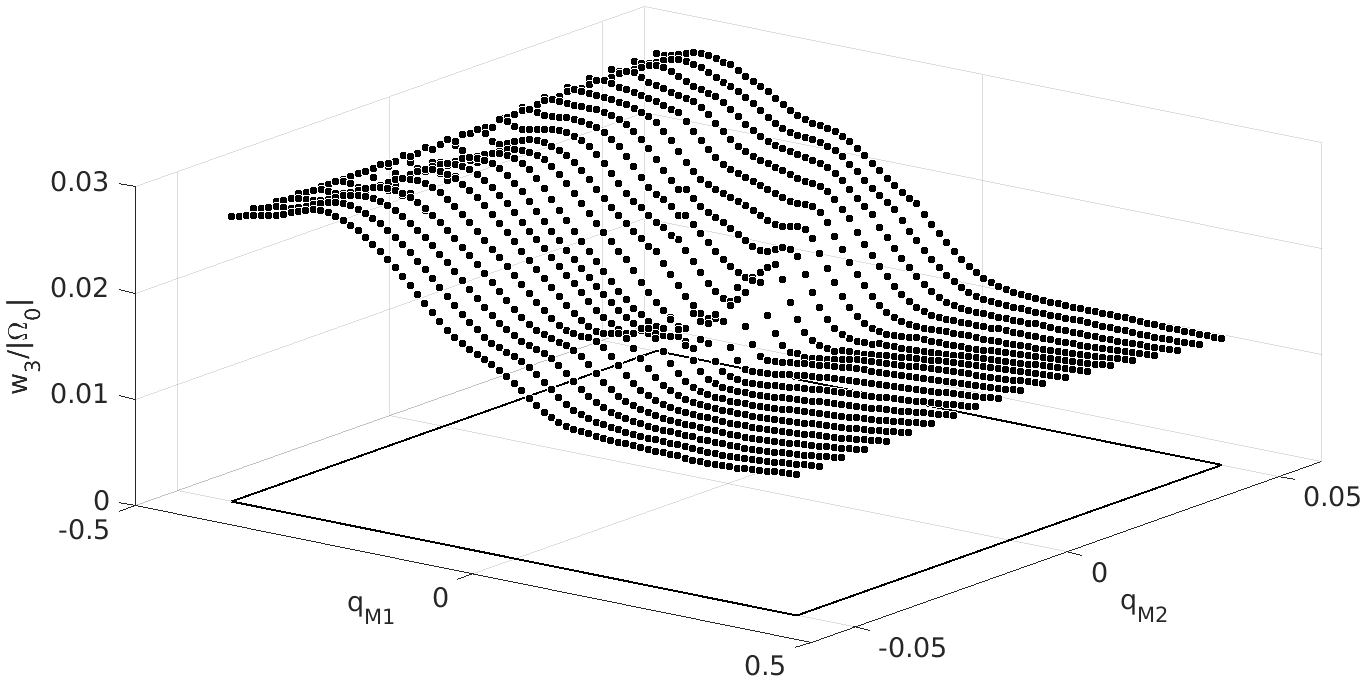
\includegraphics[width=0.48\textwidth]{FIGS/w3_alpha1e4.png} \label{fig:r}}
\caption{Sampled values of the third adaptive weight field obtained without graph regularization ($\alphaG=0$, left) and with graph regularization ($\alphaG=10^{4}$, right).}
\label{fig:w3_alpha_comparison}
\end{figure}


\begin{table}[H]
\centering
\caption{Influence of graph regularization on the accuracy of the adaptive cubature rule. Errors correspond to averages over the two training trajectories.}
\label{tab:MAW_ECM_accuracy}
\begin{tabular}{lccc}
\toprule
Model & $\nECM$ & $\errdisp$ & $\errPK$ \\
\midrule
M-HROM, fixed-weight ECM & 54
& $7.87\cdot10^{-5}$
& $2.98\cdot10^{-4}$ \\

MAW--ECM ($\alphaG=10^{4}$) & 10
& $7.87\cdot10^{-5}$
& $7.21\cdot10^{-4}$ \\

MAW--ECM ($\alphaG=0$) & 10
& $7.87\cdot10^{-5}$
& $5.21\cdot10^{-3}$ \\
\bottomrule
\end{tabular}
\end{table}




 A more quantitative assessment of the role of graph regularization is obtained by comparing the online errors shown in Table~\ref{tab:MAW_ECM_accuracy}.  The first row  reproduces the results previously reported for the fixed-weight M-HROM in Table~\ref{tab:online_fixed_manifold}, and is included here solely to facilitate a direct comparison with the adaptive cubature rules.  The displacement error $\errdisp$ remains unchanged across all three cases because the displacement   is reconstructed directly from the decoder using  (since $\qM \approx \muvec$),  and, therefore does not depend on the particular cubature rule employed. As for the error $\errPK$ in predicting homogenized PK1 stresses, we see that  reducing the support from the original $\mInit=54$ integration points to only $\nomega=10$   points   leads to an error increase with respect the to the original fixed-weight rule of  $7.21/2.98\approx 2.4$ when the regularization is active. In the absence of regularization, this error level rises up to $52.1/2.98\approx 18$.



\begin{figure}[!ht]
\centering
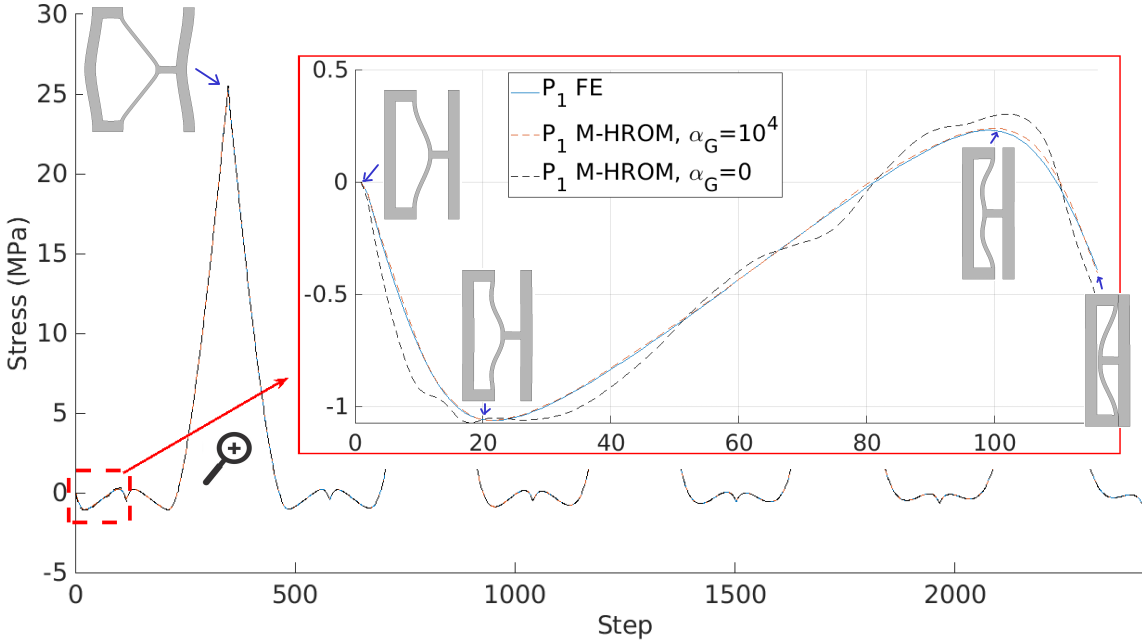
\includegraphics[width=0.7\textwidth]{FIGS/2graphs_both.png}
\caption{Comparison of the first component of the homogenized PK1 stress predicted by the FE model, the regularized MAW--ECM rule ($\alphaG=10^{4}$), and the unregularized MAW--ECM rule ($\alphaG=0$) along the second zig-zag trajectory used for training. The inset shows a magnified view of the first portion of the trajectory (steps $1$--$116$), corresponding to the compression path previously shown in Fig.~\ref{fig:adaptive_weights_compression_path}. The deformed configurations illustrate the progressive buckling of the two internal beams and the associated negative-stiffness response of the unit cell.}
\label{fig:stress_regularization_comparison}
\end{figure}


To better understand the origin of the accuracy degradation caused by the absence of regularization, we compare in  Fig.~\ref{fig:stress_regularization_comparison}   the evolution of the first component of the homogenized PK1 stress along the second zig-zag trajectory used for training. The inset provides a magnified view of the first $116$ loading steps, corresponding to the purely compressive path previously shown in Fig.~\ref{fig:adaptive_weights_compression_path}. The accompanying deformed configurations illustrate the progressive buckling of the two internal beams responsible for the apparent negative-stiffness response of the cell.

It can be readily seen that the deterioration associated with the unregularized rule is not uniformly distributed. Rather, it is concentrated in the compressive regime\footnote{It is worth noting that the global Frobenius-type error measure employed in Table~\ref{tab:MAW_ECM_accuracy} tends to attenuate the impact of these localized discrepancies because the unit cell is approximately twenty-five times stiffer in tension than in compression. Interestingly, this asymmetry is also reflected in Fig.~\ref{fig:w3_alpha_comparison}, where the strongest departures from smooth behavior occur precisely in the compressive regime ($\qMone\equiv\Gmacrox<0$).
}, as can be appreciated  in the enlarged view. Although the unregularized M-HROM prediction ($\alphaG=0$) captures the overall trend of the response, it  exhibits noticeable local deviations from the FE solution. By contrast, the regularized prediction remains in close agreement with the reference response throughout the entire compression path.


In summary, the preceding results evidence that graph regularization does improve the smoothness of the adaptive weight fields and, in doing so, also the quality of the resulting stress predictions.


% In the next section, we will consider a problem in which the latent state  cannot be recovered directly from the input parameters, but instead requires the solution of the manifold-projected reduced equilibrium equations. This will allow us to investigate the influence of the smoothness of the adaptive weights on the robustness of the Newton--Raphson scheme for solving such reduced equilibrium equations.





\section{Benchmark 2: continuum damage problem}
\label{sec:DamageProblem}
\subsection{Problem setting}
\label{sec:probsetting_2}
Having examined the performance of the proposed methodology in a
problem involving geometric nonlinearities and elastic material
behavior, we next consider a problem in which the nonlinear response
originates from inelastic constitutive effects. The benchmark selected
for this purpose is the plane-strain deformation of a plate containing
a circular hole under small-strain conditions, governed by a simple
isotropic damage model with linear hardening.  Owing to symmetry, only one quarter of the structure is
modeled, as illustrated in Figure~\ref{fig:damage_problem}(a).   A uniformly distributed traction is applied along the right boundary;  the amplitude of such a  traction, denoted by \(\fload\), is selected as
the input parameter in the problem. Displacement boundary conditions are homogeneous, and thus $\dBOUND = \zero$ in Eq.~\eqref{eq:dvecreconstruction}; likewise $\Tlift$ in the same equation reduces to  a Boolean mapping matrix from the
unconstrained degrees of freedom to the full nodal space.





The output of interest is not a derived quantity, but the state variable itself, namely the unconstrained entries
nodal displacement vector $\dred$. Unlike the Neo-Hookean-based benchmark considered in the previous
section, the constitutive memory embodied in
Eq.~\eqref{eq:damage_history_variable} prevents the solution from being
parameterized by the current value of the load factor \(\fload\)
alone. Consequently, the structural response must be recovered through
the solution of the reduced-order equilibrium equations.



Although the employed damage model
is classical, see e.g. Ref.
\cite{simo1987strain}, it is convenient to briefly recall their main
features, since they will later motivate several aspects of the
proposed  manifold HROM. In an isotropic damage model, the constitutive response at each Gauss point is driven by a single scalar
internal variable, \(\rDAMAGE\), whose evolution equation can be
integrated explicitly as follows:
\begin{equation}
\label{eq:damage_history_variable}
\rDAMAGE(t)
=
\max\left\{
\rDAMAGE(0),
\max_{0\leq s\leq t}
\sqrt{\strain(s)^{T}\Celas\strain(s)}
\right\},
\end{equation}
where  \(\strain\) and \(\Celas\) denote the infinitesimal strain vector
and the elasticity matrix, respectively.   The    damage variable  $\damage\in [0,1]$ is then recovered as $\damage =
1- {\qDAMAGE}/{\rDAMAGE}$, where
$ \dot{\qDAMAGE}
=
\hardeningD\,\dot{\rDAMAGE}$,
 \(\hardeningD\) being the hardening modulus.   The corresponding stress
vector is finally obtained as
\begin{equation}
\label{eq:damage_stress}
\stress
=
(1-\damage)\Celas\strain.
\end{equation}





\begin{figure}[htbp]
\centering
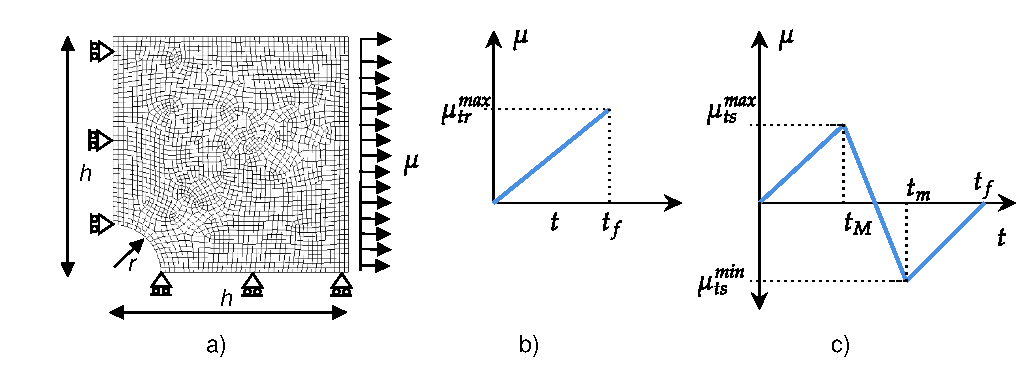
\includegraphics[width=0.95\textwidth]{FIGS/diagram_damage.pdf}
\caption{
Damage benchmark and loading trajectories.
(a) Quarter model of a plate with a circular hole
(\(h=80\,\mathrm{mm}\) and \(r=20\,\mathrm{mm}\)).  Symmetry conditions are imposed along the left
and lower boundaries, while a uniform traction of amplitude \(\fload\)
is applied on the right boundary.
(b) Training trajectory used for the construction of the HROMs.
(c) Testing trajectory employed for model validation, involving loading,
unloading, and reloading stages.
}
\label{fig:damage_problem}
\end{figure}

The finite element mesh consists
of \(\nel = 2450\) quadratic quadrilateral elements (average size $2 \,\mathrm{mm}$) and \(9997\) nodes. The material  parameters are:  Young's modulus
\(\youngD=70\,\mathrm{GPa}\), Poisson ratio \(\poissonD=0.3\), damage
threshold \(\strengthD=70\,\mathrm{MPa}\), and hardening parameter
\(\hardeningD=0.01\).


Concerning training and generalization, we adopt a deliberately
parsimonious strategy: the  reduced-order models
considered in this work---namely the standard HROM, the manifold HROM,
and the proposed manifold HROM equipped with adaptive-weight
cubature---are trained exclusively on a monotonic tensile loading path
(Figure~\ref{fig:damage_problem}(b)). No unloading, reloading, or
load-reversal information is supplied as data\footnote{ By stating that no unloading,
reloading, or load-reversal information is supplied as data, we mean
that such trajectories are not included among the training snapshots.
Naturally, this deliberate choice relies on prior knowledge of the
problem; for instance,  the assumptions of small strains and isotropic damage tells us that the model is symmetric with changes of the sign of $\fload$, so there is no need to include compression data.  }. The
reduced-order models will be then challenged with a deformation history
that does contain unloading and reloading stages
(Figure~\ref{fig:damage_problem}(c)).



For the training stage, the loading parameter increases monotonically
from zero to \(\floadmax=70\,\mathrm{MPa}\) over a pseudo-time interval
\(t_f=1\) $s$, discretized using \(\nsnap=1000\)   increments.
The generalization test is performed using the non-monotonic loading
history shown in Figure~\ref{fig:damage_problem}(c), with
\(\mu^{\max}_{ts}=0.9\floadmax\) s,
\(\mu^{\min}_{ts}=-0.95\floadmax\) s, \(t_f=1 \, s\)
\(t_M=0.45 t_f\),   \(t_m=0.9 t_f\) and  \(1500\)  increments.





\subsection{Standard HROM}

%\PROMPT{\input{Prompt_stdHROM}}

%\input{stdHROMdam_v1}


% \PROMPT{\input{Prompt_stdHROM_2}}
%
% \PROMPT{\input{Prompt_stdHROM_3}}

%\input{stdHROMdam_v2}
 %\PROMPT{\input{Prompt_stdHROM_4}}

%\input{stdHROMdam_v3}


We begin the assessment by  constructing the standard   HROM (as pointed out in Section \ref{sec:meta_standard_hrom}, this model is recovered by setting   $\qM = \qrom$ and $\TAU = \qrom$
in the manifold HROM of  Section~\ref{sec:decoderENCODER}). As customary, the unconstrained displacement snapshots are
stored in the matrix
\(\Dsnap\in\mathbb{R}^{\nL\times\nsnap}\), where, in this case,
\(\nL=19832\). The reduced basis
\(\PhiROM\) is then sought as a linear combination of the columns of
\(\Dsnap\).  In contrast to the metamaterial example, however, \(\PhiROM\) is not
obtained directly from the singular value decomposition of
\(\Dsnap\). Instead, we follow the procedure introduced by the first author in
Ref.~\cite{hernandez2014high} for elastoplastic problems, and herein
adapted to the present damage setting, whereby the displacement vector
is decomposed into a linear reference contribution and an orthogonal
nonlinear correction:
\begin{equation}
\label{eq:decomNON}
 \dred = \dredLIN + \dredNON, \qquad \textrm{where}   \qquad  {\dredLIN}^T\dredNON = 0.
\end{equation}
The component \(\dredLIN\) represents the projection of the solution
onto the undamaged subspace, whereas \(\dredNON\) contains the
remaining information associated with damage. Separate reduced bases are then constructed for each contribution. This
requires distinguishing between the undamaged and damaged portions of
the response. Accordingly, the displacement snapshots are partitioned
into two submatrices:
\begin{equation}
\label{eq:dsnapDECOMPOSITION}
 \Dsnap = \rowdos{\DsnapLIN}{\DsnapNON}
\end{equation}
  corresponding to
the undamaged regime,$\DsnapLIN$,  and the subsequent
nonlinear regime, $\DsnapNON \in \RRn{\nL}{\nsnapNON}$ (for this case, $\nsnapNON =678$).   The snapshots in \(\DsnapLIN\) are compressed without truncation,
yielding the orthonormal basis \(\PhiROMlin \), which in the present case consists
of a single mode (because there is only parameter defining the input loads). The remaining snapshots \(\DsnapNON\) are then
projected onto the orthogonal complement of \(\PhiROMlin\), producing
the residual matrix \(\DsnapNONorth\). A truncated singular value
decomposition is subsequently applied to \(\DsnapNONorth\), and the
corresponding left singular vectors define the basis
\(\PhiROMnon\). Hence,
\begin{equation}
\label{eq:bothdecom2s}
\dredLIN
=
\PhiROMlin \qMlin,
\qquad
\dredNON
\approx
\PhiROMnon \qNONall.
\end{equation}
where $\qMlin \in \Rn{}$ and $\qNONall \in \Rn{\rROM -1}$ are the corresponding linear and nonlinear amplitudes.

\begin{figure}[htbp]
\centering
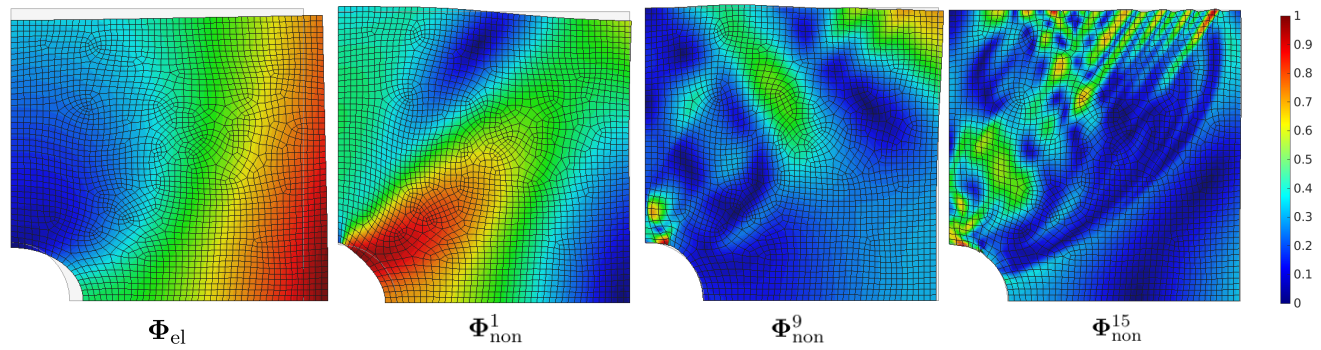
\includegraphics[width=1\textwidth]{FIGS/damage_modes.png}
\caption{
Elastic mode \(\PhiROMlin \in \Rn{\nL}\) and three representative nonlinear modes
from \(\PhiROMnon \in \RRn{\nL}{\rROM-1}\) ($\nL = 19832$, $\rROM = 16$), obtained from the displacement snapshots   generated
along the monotonic training trajectory shown in
Figure~\ref{fig:damage_problem}(b). The deformed configurations are displayed together with contour plots
of the Euclidean norm,normalized by its maximum value.
}
\label{fig:damage_modes}
\end{figure}

Using a relative truncation tolerance \(\tolSVDd=10^{-4}\), this
procedure yields 15 damage-correction modes. The resulting reduced
basis and associated generalized coordinates $\qrom$ are therefore
\begin{equation}
\label{eq:hromdamage}
\PhiROM
=
\left[
\PhiROMlin
\;
\PhiROMnon
\right], \qquad   \qrom = \coldos{\qMlin}{\qNONall},  \qquad \qrom = \PhiROM^T \dred,
\end{equation}
with a total dimension of \(\rROM=16\). Note that, by construction,
\begin{equation}
\label{eq:orthcond23}
{\PhiROMlin}^T\PhiROMnon=\bm{0}, \hspace{1cm}  {\PhiROMlin}^T\PhiROMlin=\ident,  \hspace{1cm} {\PhiROMnon}^T\PhiROMnon=\ident.
\end{equation}
By way of illustration, we show in Figure~\ref{fig:damage_modes}  the linear mode
\(\PhiROMlin\) together with three representative modes from
\(\PhiROMnon\).

We next construct the standard fixed-weight ECM rule following
Sections~\ref{sec:fixedweight_cubature}
and~\ref{sec:fixed_weight_cubature}. The only quantity entering the cubature training matrix are the projected internal-force densities; the size of this matrix in this case is thus $\ngp \times \rROM \nsnap$, where $\ngp = 2450\cdot9=22050$ and $\rROM \nsnap = 16\cdot 1000 = 16000$.
Using the SRSVD with \(\tolSVD=10^{-5}\), we get \(2369\)
left singular vectors. Augmenting this basis with the volume constraint
in Eq.~\refeq{eq:ECM_volume_constraint}, the ECM selects \(2370\)
Gauss points distributed over \(1140\) finite elements; see
Fig.~\ref{fig:damage_hrom_std}(b).

 Despite the apparent simplicity of the problem ---driven by a single
input parameter---, the resulting reduction in terms of number of
integration points is rather low (from $\ngp = 22050$ to 2370, around $10.7\%$). The explanation behind this poor reduction may lie in the fact that the growth of damage produces
an evolving nonlinear region whose spatial support changes throughout
the loading process. From the standpoint of linear approximation, this
is analogous to the difficulties encountered in transport- and
propagation-dominated problems, where the movement or evolution of localized
features is known to result in a slow decay of singular values (see e.g. Refs.~\cite{barnett2022quadratic,barnett2023neural}). The contour plot of the damage variable \(\damage\) at the end of the
loading process and the spatial distribution of the resulting ECM
points, shown in
Figures~\ref{fig:damage_hrom_std}(a)--(b), corroborate this
interpretation, as most selected Gauss points cluster in the region
where damage is most severe.



\begin{figure}[!ht]
\centering
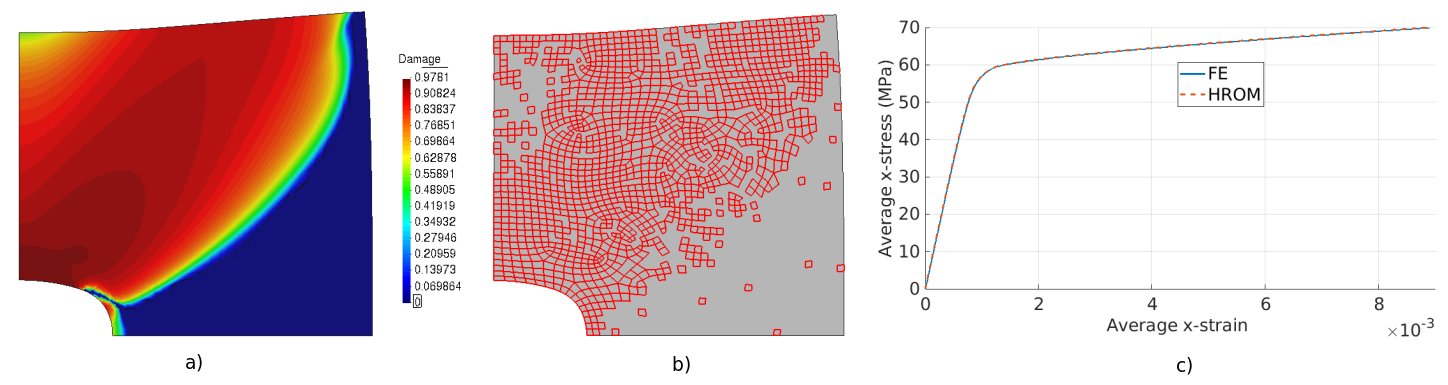
\includegraphics[width=0.95\textwidth]{FIGS/damage1.png}
\caption{Standard HROM for the damage benchmark.
(a) Damage field at the maximum training load.
(b) Elements containing the \(2370\) Gauss points selected by the
fixed ECM rule.
(c) FE and HROM average stress--strain responses along the monotonic
training trajectory.}
\label{fig:damage_hrom_std}
\end{figure}



The accuracy of the resulting HROM is assessed  using the relative
Frobenius displacement error \(\errdisp\), defined as in
Section~\ref{sec:fixedECM1}. On the training trajectory,
the standard HROM gives \(\errdisp=1.38\cdot10^{-4}\). The agreement
between the FE and HROM responses can be further appreciated  in Figure~\ref{fig:damage_hrom_std}(c), where we plot  the FE and HROM
average stress--strain curves in the loading direction. The average stress is
computed by dividing the applied force $\fload$ by the length of the loaded
boundary $h$, while the average strain is obtained from the predicted mean horizontal
displacement of the right boundary.    This graph also helps to identify the main stages of the response: an initial elastic branch is followed by a relatively sharp transition
associated with damage initiation and, subsequently, by a nonlinear
hardening regime.



As for the  generalization test of
Figure~\ref{fig:damage_problem}(c), the relative displacement error remains of the same
order, namely \(\errdisp=1.28\cdot10^{-4}\). This result corroborates our initial assumption that, for the present
benchmark, training on the monotonic tensile branch is sufficient to
capture the subsequent unloading and reloading behavior,  including the (unseen) compression regime.  The distinct stages of the cycle are illustrated   in the average stress-strain graph of Figure \ref{fig:damage_cycle}.(a), and in the evolution of the amplitudes of the three first modes, in Figure~\ref{fig:damage_cycle}(b).

 \begin{figure}[htbp]
\centering
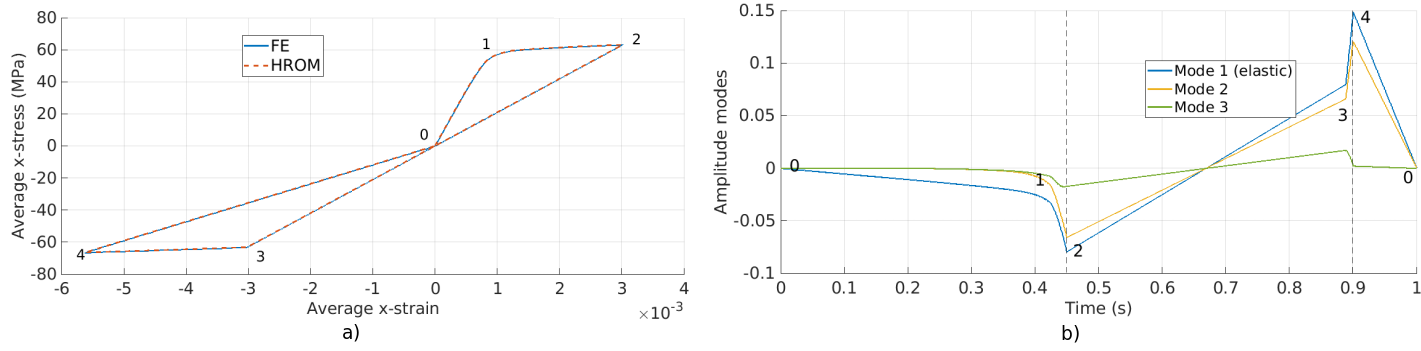
\includegraphics[width=\textwidth]{FIGS/cycle.png}
\caption{Generalization test under cyclic loading. (a) Average stress--strain response obtained during the loading cycle. The labels indicate the successive stages of the loading history: primary tensile loading (0--2), unloading from the tensile state (2--3), reverse loading into compression (3--4), and unloading from the compressive state (4--0).   (b) Evolution of the amplitudes  corresponding to  the first three modes $\PhiROM_1 = \PhiROMlin, \PhiROM_2$ and $\PhiROM_3$. }
\label{fig:damage_cycle}
\end{figure}



\subsection{Manifold HROM}
 \label{sec:meta_manifold_representation2}

%  \input{IdentLV}
%  \input{IdentLV_2}
%  \input{IdentLV_3}


\subsubsection{Identification of latent variables}
\label{sec:id2}
 Let us move now  the manifold HROM. We begin with the construction of
the decoder, for which we adopt the same master--slave structure
introduced in Eq.~\ref{eq:decoder_master_slave}, but adapted to the
linear/nonlinear decomposition of Eq.~\ref{eq:decomNON}. The latent
coordinate \(\qMlin\) and the corresponding basis matrix
\(\PhiROMlin\) for the linear component \(\dredLIN\) have already been
identified. It remains to determine how many additional latent
coordinates are required to represent the nonlinear component
\(\dredNON\), how to identify them from the training data, and,
finally, how to construct the map from the resulting master
coordinates to the slave coordinates,
\(\qS=\Nslave(\qM)\).

The constitutive response at each Gauss point is governed by a single
scalar internal variable, \(\rDAMAGE\), defined in
Eq.~\eqref{eq:damage_history_variable}. This feature, together with the
fact that the evolution of these local variables along the training
trajectory is ultimately induced by the single scalar input
\(\fload\), suggests that one additional latent coordinate may suffice
to parameterize the nonlinear component \(\dredNON\). We denote this additional
coordinate by \(\qMnon\). In accordance with the hypothesis embodied in Eq.~\ref{eq:qMdefq}, we seek $\qMnon$ as a linear combination of the
nonlinear amplitudes $\qNONall = {\PhiROMnon}^T \dred$, that is:
\begin{equation}
\label{eq:TmNONdef}
 \qMnon = \TmNON \qNONall.
\end{equation}
Thus, the problem of identifying $\qMnon$  amounts to determining the row matrix $\TmNON \in \RRn{1}{(\rROM-1)}$. It is worth noting that, with the above choice, the transformation
matrix introduced in Eq.~\ref{eq:qMdefq} adopts the form
\begin{equation}
\Tm = \matcdos{1}{\zero}{0}{\TmNON}.
\end{equation}
%


The conditions used to determine \(\TmNON\) will not be imposed
directly on Eq.~\refeq{eq:TmNONdef}, but on its normalized counterpart,
obtained by dividing both sides of that equation by \(\qMlin\):
\begin{equation}
\label{eq:TmNONdef2}
\qMnonrel = \TmNON \qNONallrel,
\end{equation}
where
\begin{equation}
\label{eq:ratiosdEF}
\qMnonrel \defeq \dfrac{\qMnon}{\qMlin},
\qquad
\qNONallrel \defeq \dfrac{\qNONall}{\qMlin},
\qquad
\qMlin \neq 0.
\end{equation}

The rationale behind this normalization  is that  these normalized variables
remain unchanged during purely elastic loading or unloading and evolve
only when damage develops at one or more Gauss points. The
normalization therefore filters out the reversible dependence on the
loading amplitude and isolates changes associated with the evolution
of damage. This property follows directly from the nature of the employed damage model. Whenever the
internal variable \(\rDAMAGE\) in Eq.~\eqref{eq:damage_history_variable}, and consequently the damage variable
\(\damage\), remain frozen at all Gauss points, the structure responds
elastically with the fixed degraded stiffness implied by
Eq.~\ref{eq:damage_stress}. The reduced amplitudes are then proportional
to the input force $\fload$ and vanish at the same zero-load
state (as can be appreciated in Fig. \ref{fig:damage_cycle}(b), between states 2 and 3) ; hence, the ratios defined in Eq.~\ref{eq:ratiosdEF} remain
constant.






 Having clarified the role of the normalization, we now turn to the
determination of \(\TmNON\). We restrict attention to the portion of
the training trajectory over which damage evolves, represented by the
nonlinear snapshot block \(\DsnapNON\), see Eq.~\ref{eq:dsnapDECOMPOSITION}, whose columns corresponds to the ordered load
levels
\begin{equation}
\label{eq:ordered}
\floadNON{1}
<
\floadNON{2}
<
\cdots
<
\floadNON{\nsnapNON},
\end{equation}
where \(\floadNON{1}\) marks the onset of damage, and
\(\floadNON{\nsnapNON} = \floadmax\) is the maximum load. The desired latent coordinate
\(\qMnonrel=\TmNON\qNONallrel\) must parameterize this one-dimensional
trajectory so that every component of \(\qNONallrel\) can be expressed
as a single-valued function of \(\qMnonrel\).  This requires \(\qMnonrel\) to be injective with respect to the applied
load \(\fload\), which in this case  amounts to require strict monotonicity of
\(\qMnonrel\) with respect to \(\fload\).







  Monotonicity is the desired outcome, but not the quantity that we
enforce directly. Instead, we seek  $\TmNON$ as the coefficients associated
with the smoothest linear combination, on the grounds that oscillatory coordinates are incompatible with the
monotonicity requirement. The   resulting optimization problem leads to  the generalized eigenvalue
problem
\begin{equation}
\label{eq:damage_graph_eig}
(\QNONrel\KGsM\QNONrel^{T})\bm{v}_i
=
\lambda_i\,
(\QNONrel\QNONrel^{T})\bm{v}_i,
\qquad
i=1,\ldots,\rROM-1.
\end{equation}
Here, $\KGsM \in \RRn{\nsnapNON}{\nsnapNON}$ denotes the graph-Laplacian operator  associated with the sequence of loads
\(\{\floadNON{i}\}_{i=1}^{\nsnapNON}\), whereas $\QNONrel\in\RRn{(\rROM-1)}{\nsnapNON}$ is obtained by dividing each column of $\Qnon = {\PhiROMnon}^T \DsnapNON$ by the corresponding entries of $\Qlin = {\PhiMlin}^T \DsnapNON$.
 The desired coefficients are finally chosen as
\begin{equation}
\label{eq:aplha}
\TmNON
=
\dfrac{\bm{v}_1^T}
{\normd{\PhiROMnon \bm{v}_1}},
\end{equation}
where \(\bm{v}_1\) is the eigenvector associated with the smallest
eigenvalue. The normalization by
\(\normd{\PhiROMnon \bm{v}_1}\) ensures that
\(\Am=\ident\) in Eq.~\ref{eq:decoder_master_slave}.

 \begin{remark}
The eigenvalue problem~\refeq{eq:damage_graph_eig} is a standard
construction in spectral graph theory; see, e.g.,
\cite{spielman2019spectral}. In the present problem, it arises from interpreting the ordered
load samples \(\{\floadNON{i}\}_{i=1}^{\nsnap}\) as the nodes of a
one-dimensional graph, and the rows of \(\QNONrel\) as scalar fields
defined on those nodes. Within this interpretation, the quadratic form
appearing in the left-hand side of Eq.~\refeq{eq:damage_graph_eig}  represents the
graph-Dirichlet energy (the same energy introduced when dealing with the regularization of the MAW-ECM in section \ref{sec:regoptprobl}), whereas the
quadratic form  in the right-hand side provides a
measure of its magnitude. The objective is therefore to find the
linear combination with minimum graph-Dirichlet energy among all
linear combinations of unit magnitude. This constrained minimization
problem takes the form of a Rayleigh quotient \cite{spielman2019spectral}, whose optimality
conditions are precisely Eq.~\refeq{eq:damage_graph_eig}. In the present one-dimensional setting, the graph-Laplacian operator $\KGsM$ can be interpreted as the stiffness (Laplacian) matrix  of a one-dimensional finite-element mesh whose nodes coincide with the ordered load samples.
\end{remark}


\begin{figure}[htbp]
\centering
 \begin{subfigure}[b]{0.48\textwidth}
\centering
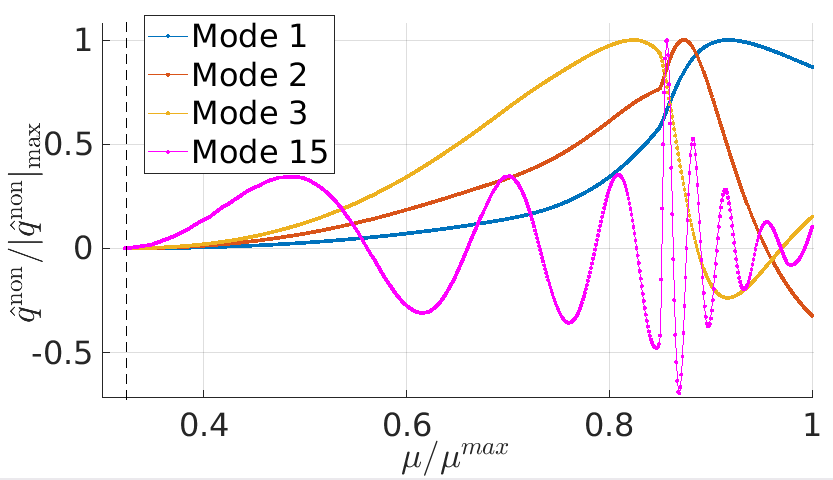
\includegraphics[width=\textwidth]{FIGS/Indiv_q.png}
\caption{}
\label{fig:damage_individual_coordinates}
\end{subfigure}
\hfill
\begin{subfigure}[b]{0.48\textwidth}
\centering
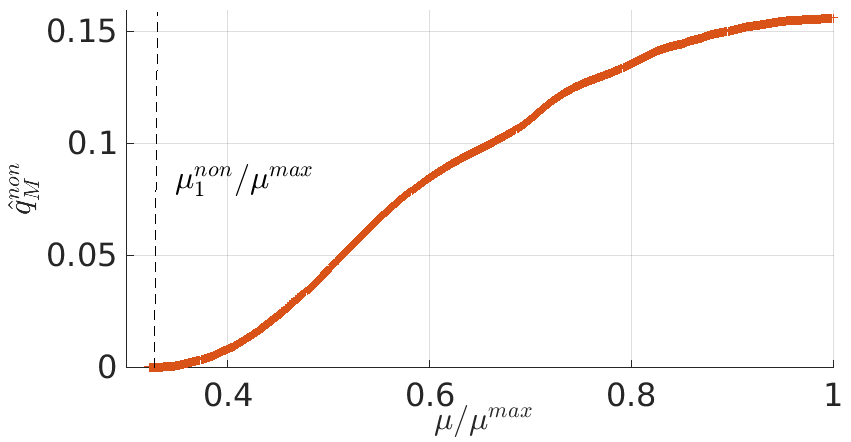
\includegraphics[width=\textwidth]{FIGS/qCHOSEN.png}
\caption{}
\label{fig:damage_selected_coordinate}
\end{subfigure}
 \caption{Identification of the nonlinear latent coordinate for the
damage benchmark. The horizontal axis represents the normalized load
parameter \(\mu/\mu^{\max}\) for the nonlinear portion of the training
tensile test (see expression~\ref{eq:ordered}). (a) Components \(1\), \(2\), \(3\), and \(15\) of the
normalized nonlinear coordinate vector
\(\qNONallrel\in\Rn{\rROM-1}\), where \(\rROM=16\); see
Eq.~\refeq{eq:ratiosdEF}. (b) Normalized latent variable $\qMnonrel$ obtained as a linear combination of $\qNONallrel$ ($\qMnonrel = \TmNON \qNONallrel$). The matrix of coefficients in this linear combination, $\TmNON$,  is determined by solving    the generalized
eigenvalue problem \eqref{eq:damage_graph_eig}.  }
 \label{fig:damage_latent_coordinate}
\end{figure}

 Figure~\ref{fig:damage_latent_coordinate} provides an a posteriori
illustration of the identification. The   components of $\qNONallrel$ shown
in Fig.~\ref{fig:damage_individual_coordinates} fail to satisfy the
monotonicity requirement and are therefore unsuitable as scalar latent
coordinates (although not shown, the remaining components  also fail to satisfy the monotonicity requirement). By contrast, the linear combination associated with the
smallest generalized eigenvalue, shown in
Fig.~\ref{fig:damage_selected_coordinate}, exhibits the desired
monotone evolution. Thus, for the present benchmark, the adopted
smoothness criterion successfully yields an injective parametrization
of the normalized nonlinear trajectory.





%\input{IdentLV_5}
%\input{IdentLV_6}
%\input{IdentLV_7}
%\input{IdentLV_8}
%\input{IdentLV_9}
\subsubsection{Nonlinear closure}
\label{sec:nonlinearclosure2}
Consistently with the normalization introduced above, we express the
closure map \(\Nslave=\Nslave(\qMlin,\qMnon)\) appearing in the decoder
of Eq.~\refeq{eq:decoder_master_slave} in the multiplicative form
\begin{equation}
\label{eq:nslave_map}
\Nslave(\qMlin,\qMnon)
=
\qMlin\,\NslaveONE(\qMnonrel).
\end{equation}
The map \(\NslaveONE=\NslaveONE(\qMnonrel)\) is constructed from the
input--output pairs  $\{\qMnonrel(\floadNON{j}), \gSnon(\floadNON{j})\}_{j=1}^{\nsnapNON}$, where $\gSnon(\floadNON{j})$ contains the normalized slave amplitudes:
\begin{equation}
\label{eq:gSnon_snap}
\gSnon(\floadNON{j})
=
\dfrac{{\PhiS}^{T}\dred(\floadNON{j})}
{\qMlin(\floadNON{j})}.
\end{equation}


The condition \(\qMlin=0\) occurs at zero applied load. Apart from the
initial state, it is encountered when the load passes through zero during
unloading. Since \(\qMnonrel\) remains constant throughout unloading, we
resolve the resulting indeterminacy by retaining its value from the
previous converged increment:
\begin{equation}
\label{eq:qMnonrel_zero}
\qMnonrel(t_{n+1})
=
\qMnonrel(t_n),
\qquad
\text{if}
\qquad
\qMlin(t_{n+1})=0,
\end{equation}
with \(\qMnonrel(0)=0\), where \(t_n\) denotes the pseudo-time of the
\(n\)-th load increment.


With the multiplicative closure in Eq.~\refeq{eq:nslave_map}, the
generic coefficient map in Eq.~\refeq{eq:tau_master_slave} specializes to
\begin{equation}
\label{eq:PhiTAU_damage}
 \TAU(\qM)
=
\begin{bmatrix}
\qMlin &
\qMnon &
\qMlin\,\NslaveONE(\qMnonrel)^T
\end{bmatrix}^T,
\end{equation}
 where \(\qMnonrel=\qMnon/\qMlin\) for \(\qMlin\neq0\), with its value
at \(\qMlin=0\) defined by Eq.~\refeq{eq:qMnonrel_zero}. Its Jacobian, see Eq.~\refeq{eq:JTAU}, follows directly from the
chain rule:
\begin{equation}
\label{eq:JTAU_damage}
\JTAU
=
\begin{bmatrix}
1 & 0\\[1mm]
0 & 1\\[1mm]
\NslaveONE(\qMnonrel)
-\qMnonrel\,\NslaveONEder(\qMnonrel)
&
\NslaveONEder(\qMnonrel)
\end{bmatrix}.
\end{equation}
Interestingly, the dependence on the master coordinates enters only
through the normalized coordinate \(\qMnonrel\). Hence, the tangent
basis \(\PhiD=\PhiROM\JTAU\), defined in
Eq.~\refeq{eq:PhiD_tau_generic} and used to project the equilibrium
residual, see Eq.~\refeq{eq:rDec_definition}, remains unchanged during elastic unloading and reloading at
frozen damage, since we have argued that \(\qMnonrel\) remains constant along
these branches.





\begin{figure}[htbp]
\centering
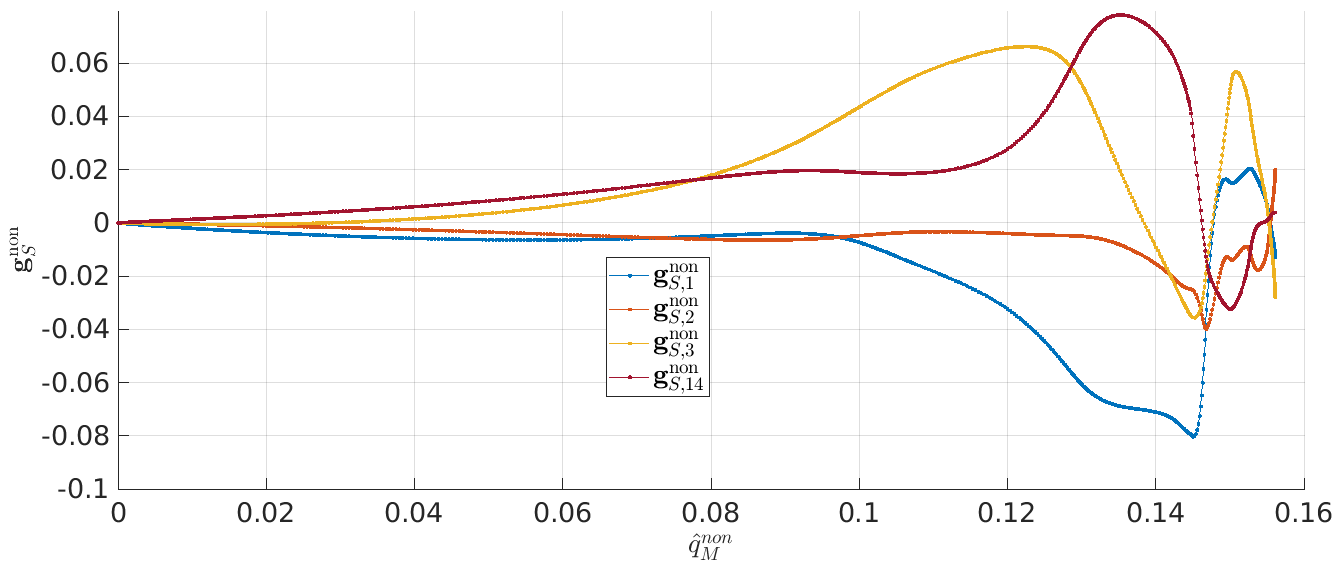
\includegraphics[width=0.7\textwidth]{FIGS/gSELEC.png}
\caption{Normalized slave amplitudes \(\gSnon\), defined in
Eq.~\refeq{eq:gSnon_snap}, as functions of the normalized latent
coordinate \(\qMnonrel\). This dataset is used for  regressing the mapping   component \(\NslaveONE = \NslaveONE(\qMnonrel)\) in Eq.~\ref{eq:nslave_map}  .}
\label{fig:damage_decoder_data}
\end{figure}


 Figure~\ref{fig:damage_decoder_data} displays four representative
normalized slave amplitudes, \(\ggSnon{i}\) (\(i=1,2,3,14\)), as
functions of \(\qMnonrel\). They vary smoothly over most of the training
range, with localized oscillations and kinks appearing only near the
final, strongly damaged states. To prevent these irregularities from
producing oscillatory decoder derivatives in
Eqs.~\refeq{eq:JTAU_damage}, we fit \(\NslaveONE\) using \(100\)
uniformly distributed samples from the \(\nsnapNON=678\) snapshots and
cubic least-squares B-splines with \(90\) knots. The resulting smoothing
error will be assessed in the following subsection (when discussing Table \ref{tab:online_fixed_manifold_damage}). Outside the
training interval, the spline is extended by a quadratic Taylor
expansion at the corresponding endpoint.




\subsubsection{Fixed-weight ECM}
\label{sec:fixedECM2}
%
% \input{ECMfix}
 %\input{ECMfix_2}


 Having defined the latent coordinates and the associated slave closure,
we now construct the fixed-weight ECM rule of
Section~\ref{sec:fixedweight_cubature}.  Since the present benchmark involves no volumetric output of interest,
we adopt the equilibrium-only case of Eq.~\refeq{eq:approxGEN}, for
which \(\rGENg{g}=\rDec{g}\) and \(\ncond=\rD=2\). Accordingly, the
training matrix \(\Agen\) of Eq.~\refeq{eq:AgenDEF} contains
only the projected internal-force densities and has dimensions
\(\Agen\in\mathbb{R}^{22050\times2000}\).  Using the SRSVD with
\(\tolSVD=10^{-5}\), and augmenting the resulting basis with the volume
constraint in Eq.~\refeq{eq:ECM_volume_constraint}, the ECM yields a
fixed rule with \(\mInit=277\) Gauss points distributed over \(213\)
finite elements, see Fig.~\ref{fig:damage_mhrom_fixed_ecm}(a).

Table~\ref{tab:online_fixed_manifold_damage} compares the online
complexity and accuracy of the resulting manifold HROM with those of
the standard HROM. The errors are the relative Frobenius displacement
errors over the monotonic training trajectory and the cyclic
generalization trajectory, respectively.

\begin{table}[!ht]
\centering
\caption{Online complexity and displacement accuracy of the fixed-weight
manifold HROM for the damage benchmark, together with the standard
HROM.}
\label{tab:online_fixed_manifold_damage}
\begin{tabular}{lccccc}
\toprule
Model
& Master coords.
& Slave coords.
& Integ. points
& \((\errdisp)^{\mathrm{train}}\)
& \((\errdisp)^{\mathrm{test}}\) \\
\midrule
HROM, ECM
& \(16\) & \(0\) & \(2370\)
& \(1.38\cdot10^{-4}\)
& \(1.28\cdot10^{-4}\) \\
M-HROM, fixed ECM
& \(2\) & \(14\) & \(277\)
& \(1.78\cdot10^{-3}\)
& \(1.81\cdot10^{-3}\) \\
\bottomrule
\end{tabular}
\end{table}

The manifold HROM reduces the number of independent coordinates from
\(\rROM=16\) to \(\rD=2\), and the number of integration points from
\(2370\) to \(277\). As in the first benchmark, the corresponding
compression factors are nearly identical, namely \(8\) and
approximately \(8.6\), respectively.

On the other hand, according to Table~\refeq{tab:online_fixed_manifold_damage}, the displacement errors increase by approximately one order of
magnitude relative to the standard HROM, but remain nearly identical
over the training and generalization trajectories. These results
indicate that the dominant additional error arises from the smoothing
introduced in the closure regression discussed in Section~\ref{sec:nonlinearclosure2}, rather
than from a loss of generalization over the unseen cyclic trajectory. Moreover, quadratic
Newton convergence was observed at every load increment.

Figure~\ref{fig:damage_mhrom_fixed_ecm}(b) further compares the latent
coordinates predicted by the manifold HROM along the generalization
trajectory with those obtained by applying the encoder in
Eq.~\refeq{eq:encoder_explicit} to the FE solutions. The linear
coordinates are virtually indistinguishable, whereas
\(\qMnonrel\) exhibits only minor discrepancies near the onset of
damage.

% \begin{remark}
% \label{remark:interpretation}
% Although \(\qMnonrel\) was introduced solely to parameterize the
% nonlinear closure, its evolution admits a direct mechanical
% interpretation. It remains constant whenever damage is frozen and
% increases only as damage develops, thus mirroring the evolution of the
% constitutive history variable \(\rDAMAGE\) in
% Eq.~\refeq{eq:damage_history_variable}. It may therefore be viewed as a
% structural-scale damage variable.
% \end{remark}


\begin{remark}
\label{remark:interpretation}
Although introduced solely to parameterize the nonlinear closure in Eq.~\refeq{eq:nslave_map},
\(\qMnonrel\) exhibits in
Figure~\ref{fig:damage_mhrom_fixed_ecm}(b) a behavior that admits a
compelling physical interpretation: as anticipated, it remains constant
during elastic unloading and reloading and, furthermore, increases
steadily as damage progresses. This is the same behavior exhibited by
the variable \(\rDAMAGE\) at the Gauss-point level; see
Eq.~\refeq{eq:damage_history_variable}. Thus, in seeking a maximally
compressed parametrization of the displacement manifold, we have
identified the structural-scale counterpart of the local internal
variable \(\rDAMAGE\).
% It should be emphasized that no phenomenological evolution law is
% postulated for this quantity. Rather, it is derived from the two latent
% coordinates obtained by solving the \(\rD=2\) projected equilibrium
% equations in Eq.~\refeq{eq:manifold_ROM_equilibrium_FE_weights}. Its
% irreversible, history-recording character therefore emerges from the
%reduced equilibrium problem itself.
\end{remark}

\begin{figure}[htbp]
\centering
\begin{subfigure}[t]{0.28\textwidth}
\centering
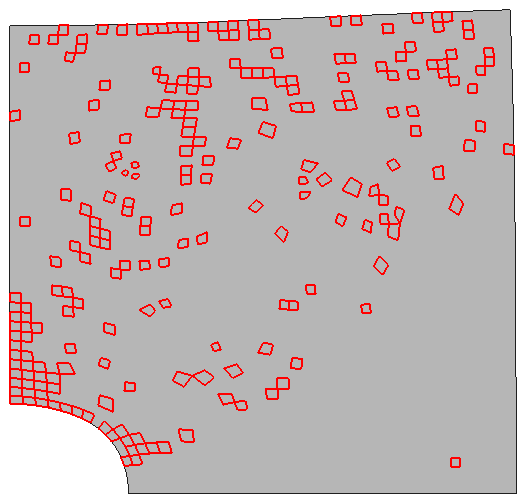
\includegraphics[width=\textwidth]{FIGS/MHROM_ECMfixed.png}
\caption{Elements containing the selected Gauss points.}
\label{fig:ECM_FIXED2}
\end{subfigure}
\hfill
\begin{subfigure}[t]{0.62\textwidth}
\centering
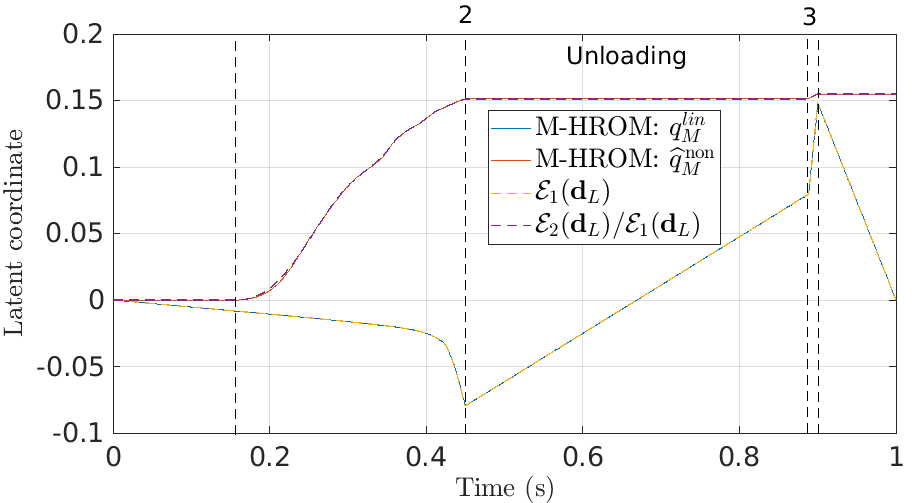
\includegraphics[width=\textwidth]{FIGS/vinterna3.png}
\caption{Latent coordinates along the generalization trajectory.}
\label{fig:vinterna3}
\end{subfigure}
\caption{Fixed-weight manifold HROM for the damage benchmark.
(a) Elements containing the \(277\) Gauss points selected by the ECM.
(b) Evolution of \(\qMlin\) and \(\qMnonrel\) along the generalization
trajectory of Fig.~\ref{fig:damage_problem}(c), compared with the
coordinates obtained by applying the encoder in
Eq.~\refeq{eq:encoder_explicit} to the FE solutions.}
\label{fig:damage_mhrom_fixed_ecm}
\end{figure}


\subsection{Manifold-adaptive weight ECM }
\PROMPT{\input{Prompt_MAWD1}}
%\input{MAWD1}
%
% We now apply the MAW--ECM methodology described in
% Box~\ref{box:MAW_ECM_summary} to the manifold-HROM associated with the
% present damage benchmark.  We assume that the adaptive weights   depend exclusively on the
% normalized nonlinear coordinate \(\qMnonrel\):
% \begin{equation}
% \label{eq:normalizedTRAININGw}
% \omegag{g}=\omegag{g}(\qMnonrel),
% \qquad
% g\in\Zomega.
% \end{equation}
%
% To ensure that the adaptive weights are consistent with the functional dependence defined in the preceding equation, the desired cubature rule must integrate
% exactly the virtual internal work associated with the virgin elastic
% response  ---because, in this regime, $\qMnonrel=0$, and  the response  depends only on $\qMlin$. To this end, we first    partition  the training matrix of internal-work densities \(\AforceD\), defined in Eq.~\refeq{eq:AforceD_training_matrix},    into  linear and nonlinear blocks:
% \begin{equation}
%  \AforceD = \rowdos{\AforceDlin}{\AforceDnon}.
% \end{equation}
% Then we apply the SVD over the linear block $\AforceDlin$; let $\Uel$ be the matrix of left singular vectors arising from such SVD (which will have $\rD = 2$ vectors due to the linearity of the problem in this regime).   The required condition can be finally enforced by expanding the invariant matrix
%  introduced in Eq.~\eqref{eq:invariants1} with $\Uel$, i.e.:
% \begin{equation}
% \label{eq:Uinv_damage}
% \Uinv=
% \left[
% \Uel,\,
% \onevec
% \right].
% \end{equation}
% %

We now apply the MAW--ECM methodology summarized in
Box~\ref{box:MAW_ECM_summary} to the manifold HROM of the present
damage benchmark. Consistently with the normalized manifold
parametrization, we choose the adaptive weights to depend only on
\(\qMnonrel\):
\begin{equation}
\label{eq:normalizedTRAININGw}
\omegag{g}=\omegag{g}(\qMnonrel),
\qquad
g\in\Zomega.
\end{equation}

% \begin{equation}
% \label{eq:dsnapDECOMPOSITION}
%  \Dsnap = \rowdos{\DsnapLIN}{\DsnapNON}
% \end{equation}

This choice assigns the same weight vector to all states of the virgin
elastic branch, for which \(\qMnonrel=0\) while \(\qMlin\) varies. The
adaptive rule must therefore reproduce exactly the projected internal
forces over this branch. To enforce this requirement, we partition the
training matrix into its elastic and nonlinear blocks,
$\Agen=\rowdos{\AgenLIN}{\AgenNON}$,
analogously to the displacement-snapshot decomposition in
Eq.~\refeq{eq:dsnapDECOMPOSITION}. Let \(\Uel\) denote a basis for the
column space of \(\AgenLIN\), which, owing to the linearity of the
response in this regime, has dimension \(\rD=2\). We include this basis
among the invariant constraints of Eq.~\refeq{eq:invariants1}:
\begin{equation}
\label{eq:Uinv_damage}
\Uinv=
\left[
\Uel,\,
\onevec
\right].
\end{equation}

The nonlinear block
\(\AgenNON\in\RRn{\ngp}{\nsnapNON\rD}\) supplies the state-dependent
conditions along the damaged portion of the training trajectory. In
summary, at each sampled value \(\qMnonrel(\floadNON{j})\), the local
system comprises the \(\ncond=\rD=2\) conditions associated with the
projected internal forces, the \(\rD=2\) elastic invariants in \(\Uel\),
and the volume constraint. Hence, the lower bound defined in
Eq.~\refeq{eq:ncondmin} becomes
\begin{equation}
\label{eq:ncond_damage}
\mLower = \ncond+\ninv = \rD+\rD+1 = 5.
\end{equation}
In other words, the desired adaptive rule satisfying the local
constraints must contain at least \(\mLower=5\) integration points.

\begin{remark}
A key consequence of the proposed parametrization for the adaptive weights  is that no additional
constraints are required to describe unloading. Indeed, since \(\qMnonrel\)
remains constant during unloading,   the Jacobian matrix
\(\JTAU\) of Eq.~\eqref{eq:JTAU_damage} remains constant as well. Furthermore, according to Eq.~\eqref{eq:PhiTAU_damage},
the decoder is linear with respect to \(\qMlin\) when
\(\qMnonrel\) is fixed. Hence, all states belonging to the same
unloading branch differ only through a scalar scaling factor and,  as a result, enforcing the local integration constraints at a given damage state
of the training set automatically guarantees the same level of
integration accuracy along any unloading trajectory emanating from
that state.
\end{remark}



\subsubsection{Influence of the fixed-weight initialization and pruning efficiency}

We now proceed with the  assessment of the efficiency  of
the pruning process of
Algorithm~\ref{alg:MAW_global_pruning} for different initializations, namely three initial cubature
rules containing \(\mInit=97\), \(\mInit=277\), and
\(\mInit=534\) integration points, respectively.  These rules are obtained by varying the   truncation tolerance
\(\tolSVD\) in Eq.~\refeq{eq:Ucub_definition}, applied to the
internal-force training matrix \(\Agen\). The initial rule displayed
previously in Figure~\ref{fig:ECM_FIXED2} corresponds to the
intermediate case, \(\tolSVD=10^{-5}\), yielding \(\mInit=277\)
integration points.
The ordered samples
\(\{\qMnonrel(\floadNON{j})\}_{j=1}^{\nM}\) ($\nM = \nsnapNON$) define the nodes of
a one-dimensional latent mesh. Accordingly, the graph operator
\(\KGs\) entering the pruning algorithm is assembled from the standard
finite element discretization of the one-dimensional Laplacian using
linear shape functions, analogously to the construction of \(\KGsM\)
in Eq.~\refeq{eq:damage_graph_eig}.  The graph-regularization parameter is fixed at \(\alphaG=0.1\), and the
pruning algorithm performs \(\ntry=5\) trials per branch.




\begin{table}[ht!]
\centering
\caption{Influence of the fixed-weight initialization on the MAW--ECM
pruning process for different values of the SVD truncation tolerance
\(\tolSVDfixed\) employed in the construction of the
internal-force matrix \(\AforceD\). Here, \(\mInit\) denotes the number
of points of the initial fixed-weight ECM rule, whereas
\emph{Unregularized pruning} reports the percentage of integration
points eliminated without activating graph regularization or explicit
positivity enforcement; \(\nomega\) denotes the final number of
integration points, and \emph{Total time} corresponds to the
wall-clock time of the complete MAW--ECM pruning algorithm.}
\label{tab:maw_pruning_summary_damage}
\begin{tabular}{ccccc}
\hline
\(\tolSVDfixed\) &
\(\mInit\) &
Unregularized pruning (\%) &
\(\nomega\) &
Total time (s) \\
\hline
$10^{-4}$ & $97$  & $80.4$ & $8$ & $46.1$ \\
$10^{-5}$ & $277$ & $87.0$ & $7$ & $131.0$ \\
$10^{-6}$ & $534$ & $96.4$ & $7$ & $63.9$ \\
\hline
\end{tabular}
\end{table}

Table~\ref{tab:maw_pruning_summary_damage} summarizes the results of
the three pruning tests. Despite the large variability in the size of
the initial fixed-weight rules, all three pruning processes converge
to adaptive cubature rules containing only
\(\nomega=7\)--\(8\) integration points, i.e., just two or three
points above the theoretical lower bound \(\mLower=5\) established in
Eq.~\eqref{eq:ncond_damage}.  This is
essentially the same behavior observed in the metamaterial benchmark
(Table~\ref{tab:maw_pruning_summary}) and corroborates that the
number of integration points is dictated primarily by the intrinsic dimension
of the solution manifold, rather than by the size of the initial
fixed-weight cubature rule.





 Table~\ref{tab:maw_pruning_summary_damage} also confirms another
trend observed in the metamaterial benchmark discussed in Section \ref{sec:infl_fw_ini}: graph regularization and
explicit positivity enforcement are required only during a relatively
small fraction of the pruning iterations. Indeed, in the three
studied cases, between \(80\%\) and \(96\%\) of the integration
points are eliminated without activating the positivity-enforcement
stage of Algorithm~\ref{alg:prune_step_optionB}. It is worth noting that the   tests also revealed an
intermittent activation of the regularization stage, with the pruning
algorithm   switching between regularized and unregularized
iterations before reaching the final rule. Such behavior was not
observed in the metamaterial benchmark, where the first activation of
the positivity-enforcement stage invariably led to a permanent
transition to the regularized regime.


By way of illustration, Figure~\ref{fig:damage3cases} displays, in
the top row, the finite elements containing the integration points of
the initial fixed-weight rules considered in
Table~\ref{tab:maw_pruning_summary_damage};  the lower row, on the other hand, shows the
location of the integration points of the final sparsest rule,  superposed on the contour
plot of the  damage field  predicted by the FE model at the final step of the training trajectory.
It is interesting to note that the spatial distribution of the retained points exhibits, in all three
cases, a remarkably similar pattern: one point is invariably located
in the undamaged region (point \(1\) in
Fig.~\ref{fig:damage3cases}(b)); three or four points are placed in the vicinity of
the hole boundary, where damage nucleates and the stress
concentration is highest (points \(3\), \(4\), \(6\), and \(7\) in
Fig.~\ref{fig:damage3cases}(b)); and the other two or three points are located within the damaged region,
but away from the hole.
%
% This recurrent pattern   evidences
% that the pruning procedure does not select integration points arbitrarily, but    points that are physically relevant for capturing the
%
% does   select integration points arbitrarily, but rather it
%
%
% appears to identify, from the information contained in the internal-force density matrix, the regions of the domain carrying the most relevant information.



\begin{figure}[t]
\centering
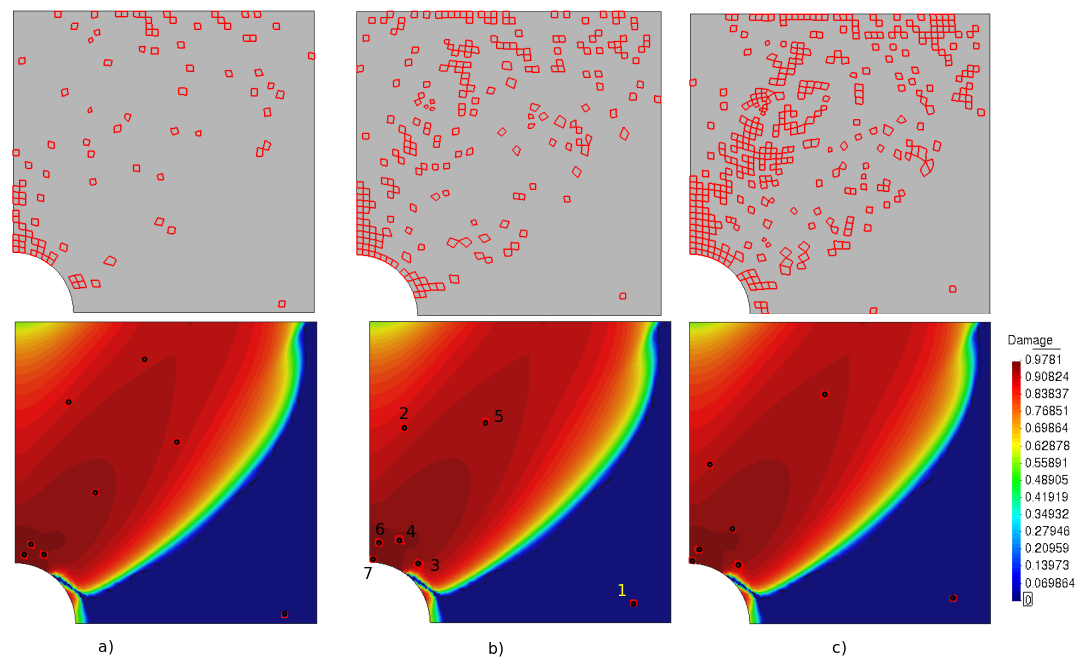
\includegraphics[width=0.9\textwidth]{FIGS/damage3cases2.png}
\caption{Spatial distribution of the integration points associated with the
initial and final cubature rules corresponding to the three
fixed-weight initializations reported in
Table~\ref{tab:maw_pruning_summary_damage}. The upper row shows the
elements containing the integration points of the initial fixed-weight
rules. The lower row shows the retained integration points of the final
adaptive rules, superposed on the damage field \(\damage\) at the end
of the training trajectory. The three columns correspond to the
initializations \(\mInit=97\), \(\mInit=277\), and \(\mInit=534\),
respectively. The labels in panel (b) identify the seven retained
points used in the subsequent analysis.}
\label{fig:damage3cases}
\end{figure}

On the other hand, Figure~\ref{fig:damage_weights_samples}(a) displays the sampled
adaptive weights
\(\{(\Wad)_{g,j}\}_{j=1}^{\nsnap}\),
\(g=1,2,\ldots,\nomega\)
(see Eq.~\eqref{eq:pairs}) computed by the MAW--ECM for the case
\(\mInit=277\). The weights are represented as functions of the
corresponding latent states
\(\{\qMnonrel(\floadNON{j})\}_{j=1}^{\nsnapNON}\). For illustration purposes, the finite elements containing the integration points
of the corresponding adaptive rule, already shown in
Fig.~\ref{fig:damage3cases}(b), are reproduced as an inset.  Inspection
of these graphs  reveals a smooth dependence
on \(\qMnonrel\) throughout most of the sampled interval, with some irregularities appearing near \(\qMnonrel=0\) (which   may be
attributed to boundary effects inherent to the graph-regularization
procedure).   Nevertheless, such irregularities are relatively minor when compared
with the behavior of the graphs obtained when the  regularization stage of
Algorithm~\ref{alg:prune_step_optionB} is disabled, in
the same spirit as the comparison reported in
Fig.~\ref{fig:w3_alpha_comparison} for the metamaterial benchmark.
The corresponding results for the present problem are shown in
Fig.~\ref{fig:damage_weights_samples}(b).  We can see that  the sampled
weights exhibit abrupt variations  and a markedly less coherent
dependence on \(\qMnonrel\) that in the regularized case, confirming    that graph
regularization  does play a crucial role in generating weight distributions which are relatively smooth, and thus
amenable to subsequent regression.

% On the other hand, Figure~\ref{fig:damage_weights_samples}
% (a) displays the sampled adaptive weights $\{(\Wad)_{g,j}\}_{g=1}^{\nsnap}$, $g=1,2 \ldots \nomega$  (see Eq. \ref{eq:pairs}), corresponding to the intermediate initialization, \(\mInit=277\), shown
% in Fig.~\ref{fig:damage3cases}(b).   The
% largest average contribution is carried by point \(1\), located in the
% undamaged region, and the dependence on $\qMnonrel$ is generally smooth.
% The mild irregularities observed near the $\qMnonrel = 0$
% are consistent with an endpoint effect of the graph regularization:
% near the boundary of the sampled interval, each weight sample is
% coupled to fewer neighboring states, and the smoothing action of the
% graph Laplacian is correspondingly weaker. However, this irregularies are  small when
% compared with the behavior obtained by suppressing the regularization in the first place (as done in Figure \ref{fig:w3_alpha_comparison} in the metamaterial benchmark),
% shown in Fig.~\ref{fig:damage_weights_samples}(b). In that case, the
% sampled weights exhibit abrupt variations and a markedly less coherent
% evolution with \(\qMnonrel\).  This comparison confirms,
% as in the metamaterial benchmark, that graph regularization o contributes to
% the construction of weight samples suitable for subsequent regression.





% We focus next on the intermediate initialization, \(\mInit=277\), shown
% in Fig.~\ref{fig:damage3cases}(b). Figure~\ref{fig:damage_weights_samples}
% (a) displays the sampled adaptive weights \((W)_{i,j}\) associated with
% the seven retained points, as functions of the normalized nonlinear
% coordinate \(\qMnonrel\). These are the weights delivered by the
% pruning algorithm, before any regression step is applied. Their
% evolution is generally smooth over most of the sampled interval. The
% largest average contribution is carried by point \(1\), located in the
% undamaged region, while the remaining weights redistribute the
% contribution of the damage-affected zone.


\begin{figure}[t]
\centering
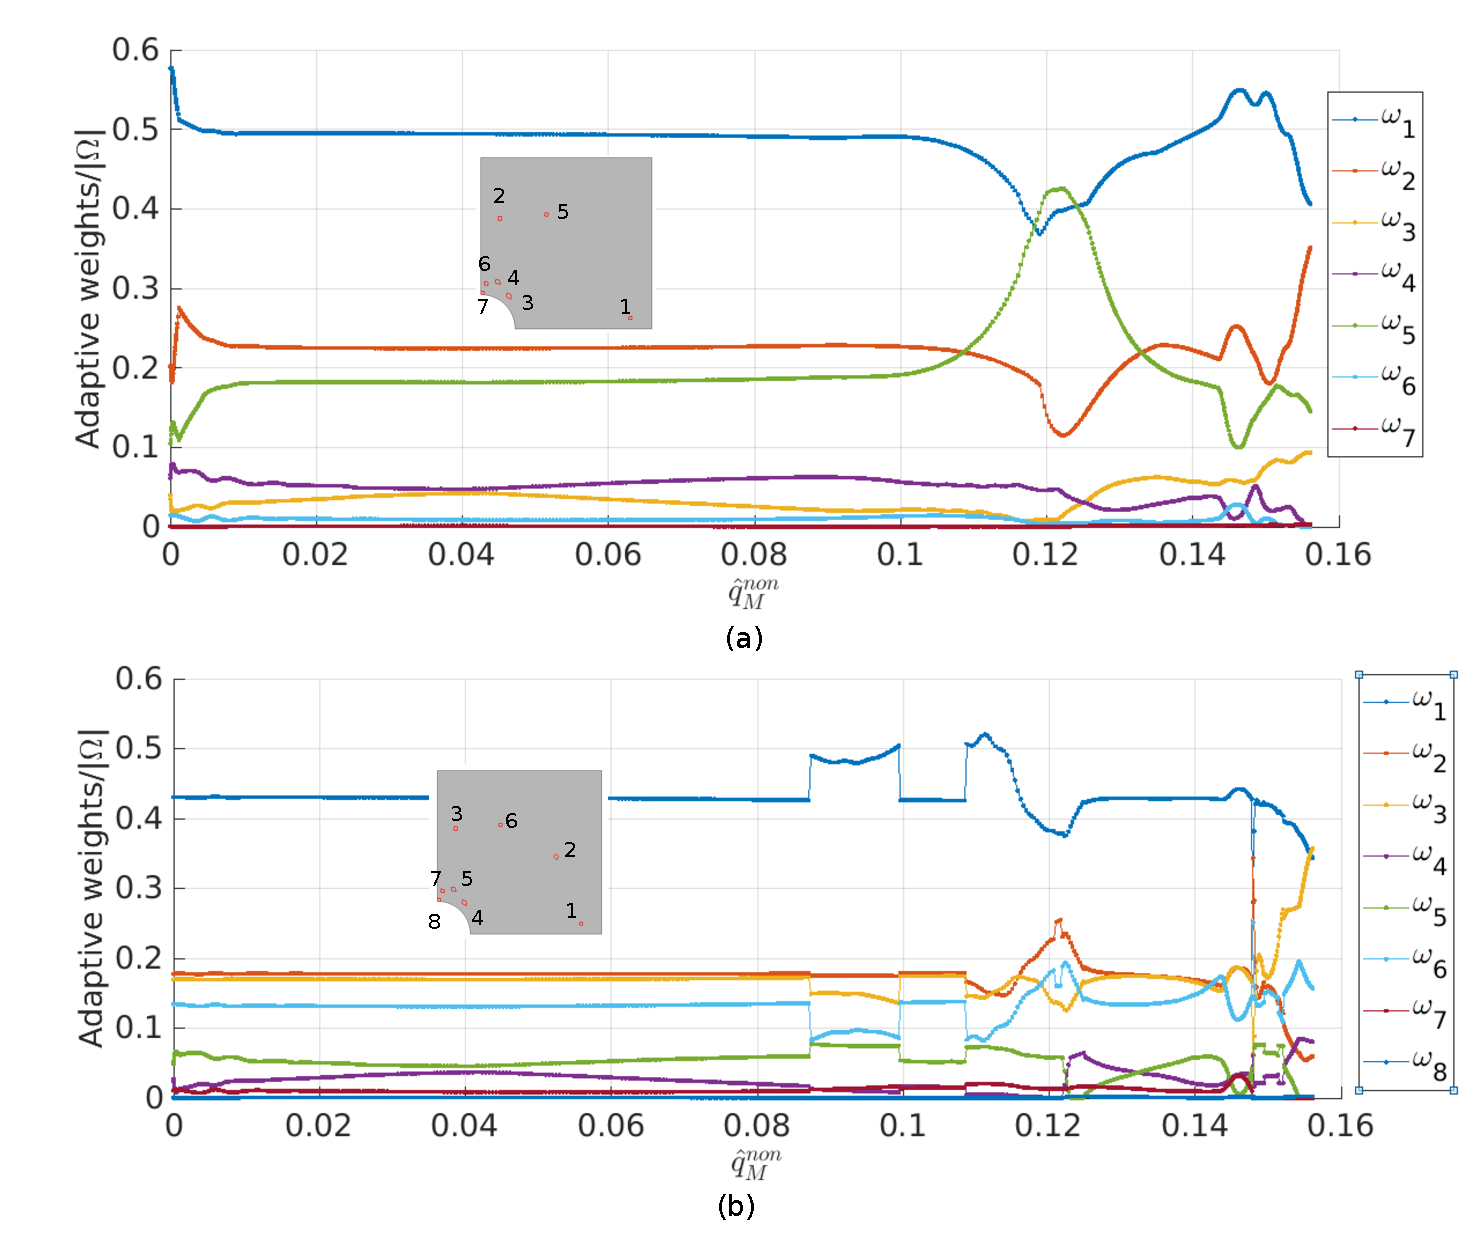
\includegraphics[width=0.8\textwidth]{FIGS/adaptive_weigths_1em5.pdf}
\caption{Sampled adaptive weights obtained from the pruning algorithm
for the damage benchmark with \(\mInit=277\).  The insets show the retained supports and the
labels used to identify the individual weight samples.  (a) Graph-regularized pruning procedure.  (b) Pruning without regularization. }
\label{fig:damage_weights_samples}
\end{figure}


The adaptive nature of the proposed cubature rules can be appreciated
more clearly in Fig.~\ref{fig:damage_pruning_path}, which displays the
sampled weights associated with four intermediate rules (with
\(\nomega=14\), \(12\), \(10\), and \(8\) integration points)
extracted along the pruning process that led to the \(\nomega=7\)
adaptive weight fields shown previously in
Fig.~\ref{fig:damage_weights_samples}(a).     To visualize the progressive evolution of the spatial distribution of
the integration points, each panel includes an inset showing the
corresponding integration rule, with circles marking the integration
points that will be removed in the subsequent pruning stage. We can
see that, as the rule is progressively pruned, the variability of the
weight curves increases.  Indeed, for \(\nomega=14\) and \(\nomega=12\), the weights exhibit
only mild variations along the latent manifold, whereas for
\(\nomega=10\) and, even more markedly, for \(\nomega=8\), they vary
more significantly with \(\qMnonrel\) to compensate for the discarded
integration points.




\begin{remark}
It should be recalled that all the rules shown in
Fig.~\ref{fig:damage_pruning_path} are feasible solutions of the
original optimization problem, i.e., they satisfy the local exactness
and positivity constraints. Consequently, if the optimal (i.e., the
sparsest) rule is deemed excessively irregular for subsequent
regression, one may deliberately step back along the pruning path and
select a denser, yet smoother, rule instead.
\end{remark}


%  The adaptive nature of the proposed cubature rules can be appreciated
% more clearly in Fig.~\ref{fig:damage_pruning_path}, which displays the
% sampled weights associated with four feasible rules (with $14$, $12$, $10$ and $8$ integration points ) extracted along the
% pruning process that led to the $\nomega=7$ adaptive weight fields shown previously in Figure \ref{fig:damage_weights_samples}.(a). To facilitate the interpretation of the results, each panel includes
% an inset showing the elements containing the integration points of the
% corresponding rule. The points enclosed by circles identify the
% integration points that will be removed in the next pruning stage.
% These insets provide a graphical representation of how the support
% evolves during the pruning process. It can be seen that for
% \(\nomega=14\) and \(\nomega=12\) the sampled weights exhibit only
% mild variations along the latent manifold, but  as the number of points is
%   reduced to $\nomega=10$ and, especially, to
% \(\nomega=8\), the effect of the eliminated integration points is
%   absorbed by the surviving ones, whose weights exhibit
% correspondingly stronger variations with \(\qMnonrel\).

% An interesting trend emerges from the figure. For relatively large
% supports (\(\nomega=14\) and \(\nomega=12\)), most weights remain
% nearly constant throughout the latent manifold, indicating that the
% available redundancy is sufficient to satisfy the local exactness
% constraints with only limited adaptation. As the support is further
% reduced (\(\nomega=10\) and, especially, \(\nomega=8\)), the remaining
% integration points must progressively compensate for the information
% lost by the removed points. Consequently, the associated weights
% become increasingly state-dependent, exhibiting stronger variations
% with \(\qMnonrel\). Thus, the reduction in the number of integration
% points is accompanied by a corresponding increase in the adaptability
% of the remaining weights.


\begin{figure}[t]
\centering
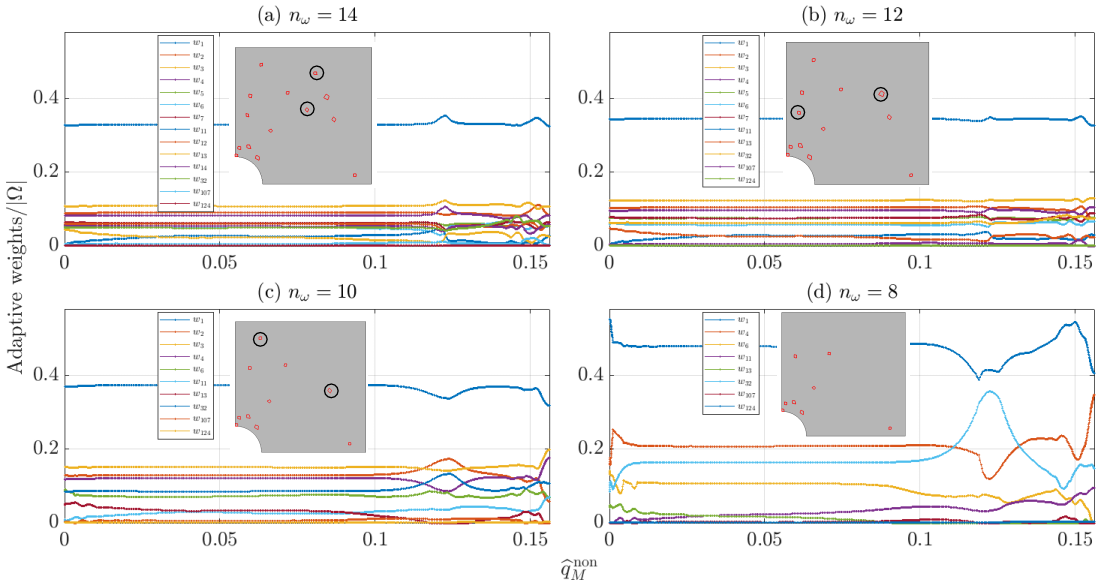
\includegraphics[width=1\textwidth]{FIGS/4fig.png}
\caption{Adaptive weights as a function of the normalized, nonlinear latent coordinate $\qMnonrel$, corresponding to four feasible
cubature rules extracted from different stages of the pruning process (containing
\(\nomega=14\), \(12\), \(10\), and \(8\) integration points).  The insets show the
elements containing the integration points of each rule. Integration
points enclosed by circles are those selected for removal in the
subsequent pruning stage.  }
 \label{fig:damage_pruning_path}
\end{figure}








%
%
% \subsubsection{Online accuracy assessment}
% \label{sec:online2}
% The online solution procedure coincides with that of the fixed-weight
% manifold HROM, except that the consistent Newton linearization must
% account for the dependence of the adaptive weights on
% \(\qMnonrel\). This introduces an additional weight-variation
% contribution to the tangent matrix, whose derivation is given in
% \ref{app:MAW_linearization}.
%
% The adaptive weight fields
% \(\omegag{g}=\omegag{g}(\qMnonrel)\) are represented using the same
% spline framework employed for the decoder in
% Section~\ref{sec:nonlinearclosure2}. The regressions use \(500\)
% uniformly distributed samples selected from the \(\nsnapNON=678\)
% available snapshots. Outside the sampled interval, each weight is held
% constant at its nearest endpoint value, thereby preserving positivity
% and the exact volume constraint inherited from the adaptive cubature
% construction.
%
%
% We conclude the assessment by examining the online response obtained
% with the adaptive rule shown in
% Figure~\ref{fig:damage_weights_samples}(a), obtained from the
% \(\mInit=277\) fixed-weight initialization and containing only
% \(\nomega=7\) integration points. The corresponding fixed-weight
% manifold HROM of Section~\ref{sec:fixedECM2} is retained as reference.
% The results are summarized in Table~\ref{tab:damage_maw_accuracy}.

\subsubsection{Online accuracy assessment}
\label{sec:online2}

We finally assess whether the substantial reduction, in terms of integration points, achieved by
MAW--ECM compromises the online accuracy of the manifold HROM. To this
end, we consider the adaptive rule shown in
Figure~\ref{fig:damage_weights_samples}(a), obtained by pruning the
\(\mInit=277\) fixed-weight rule down to only \(\nomega=7\) integration
points. The corresponding fixed-weight manifold HROM of
Section~\ref{sec:fixedECM2} (see Table~\ref{tab:damage_maw_accuracy}) is retained as reference, so that the
comparison isolates the effect of replacing the fixed cubature rule by
the adaptive one.

For online evaluation, the sampled adaptive weights
\(\omegag{g}=\omegag{g}(\qMnonrel)\) are represented using the same
spline framework employed for the decoder in
Section~\ref{sec:nonlinearclosure2}. The regressions use \(500\)
uniformly distributed samples selected from the \(\nsnapNON=678\)
available snapshots. Outside the sampled interval, each weight is held
constant at its nearest endpoint value, thereby preserving positivity
and the exact volume constraint inherited from the adaptive cubature
construction.


\begin{table}[t]
\centering
\caption{Relative displacement errors for the fixed- and
adaptive-weight manifold HROMs.}
\label{tab:damage_maw_accuracy}
\begin{tabular}{lccc}
\hline
Model
&
Number of points
&
\((\errdisp)^{train}\)
&
\((\errdisp)^{test}\)
\\
\hline
Fixed-weight manifold HROM
&
\(277\)
&
\(1.78\cdot10^{-3}\)
&
\(1.81\cdot10^{-3}\)
\\
Manifold HROM with MAW--ECM
&
\(7\)
&
\(1.8125\cdot10^{-3}\)
&
\(1.6538\cdot10^{-3}\)
\\
\hline
\end{tabular}
\end{table}

The resulting displacement errors over the training and generalization
trajectories are reported in Table~\ref{tab:damage_maw_accuracy}.
Inspection of this table shows that the adaptive rule essentially
preserves the accuracy of the fixed-weight manifold HROM: the small
variations observed in the training and test errors are negligible
relative to the approximation error already introduced by the decoder.



A more detailed assessment is provided in
Figure~\ref{fig:damage_maw_global}, which compares the latent
coordinates---the same comparison carried out in
Figure~\ref{fig:damage_mhrom_fixed_ecm}(b) for the fixed-weight
case---and the macroscopic stress--strain response along the
generalization trajectory. As in the fixed-weight case, \(\qMlin\) in
Figure~\ref{fig:damage_maw_latent} is virtually indistinguishable from
its encoded FE counterpart. The normalized nonlinear coordinate
\(\qMnonrel\), by contrast, exhibits a small but visible departure from
its encoded FE counterpart around \(t=0.2\)~s, at the onset of damage.
However, once damage evolution is fully established, the manifold-HROM
curve rejoins the reference FE curve, and the two solutions again
become indistinguishable.

The origin of the above mentioned deviation appears to lie in the weight regression:
it occurs at the onset of damage, that is,  when  \(\qMnonrel\approx0\), precisely where the sampled weights in
Figure~\ref{fig:damage_weights_samples}(a) exhibit their largest local
irregularities. Nevertheless, this local deviation has practically
no influence on the global displacement error, as confirmed by
Table~\ref{tab:damage_maw_accuracy}, nor on the macroscopic
stress--strain response shown in
Figure~\ref{fig:damage_maw_stress_strain}, where the complete macroscopic
cycle---including primary loading, unloading, reverse loading in
compression, and final unloading---is reproduced with no visible
discrepancy.

\begin{figure}[t]
\centering
\subfloat[Evolution of the latent coordinates.]{
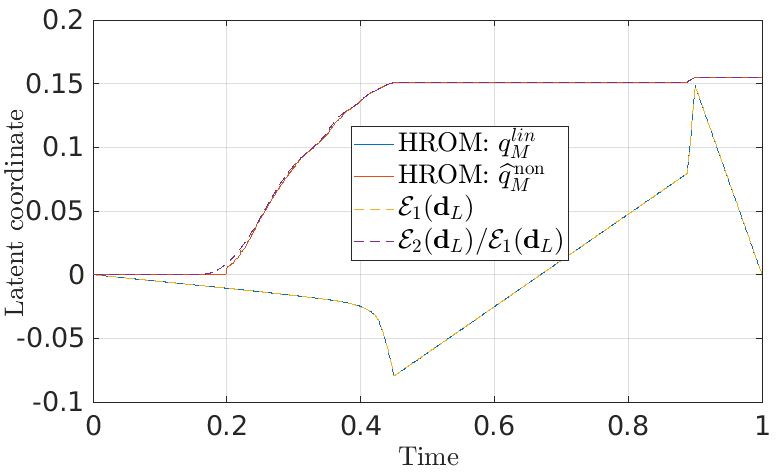
\includegraphics[width=0.5\textwidth]
{FIGS/last.png}
\label{fig:damage_maw_latent}
}
\hfill
\subfloat[Average axial stress--strain response.]{
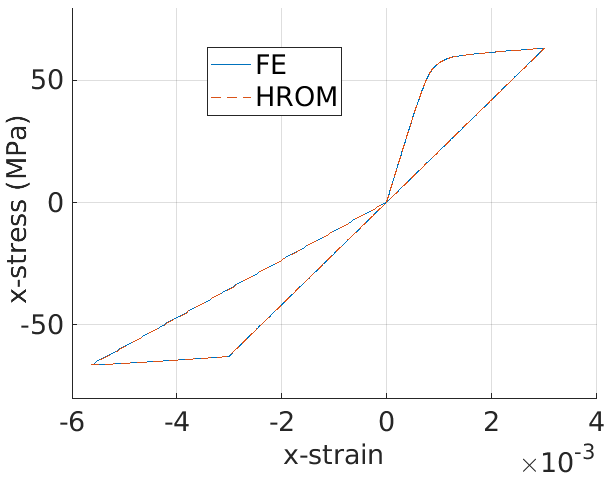
\includegraphics[width=0.40\textwidth]
{FIGS/last2.png}
\label{fig:damage_maw_stress_strain}
}
\caption{Online response of the manifold HROM with the adaptive rule of
\(\nomega=7\) integration points along the generalization trajectory of
Fig.~\ref{fig:damage_problem}(c).
(a) Evolution of \(\qMlin\) and \(\qMnonrel\), compared with the
coordinates obtained by applying the encoder in
Eq.~\refeq{eq:encoder_explicit} to the FE solutions (see Fig.~\ref{fig:damage_mhrom_fixed_ecm}(b) for the analogous
fixed-weight comparison).
(b) Average axial stress--strain response predicted by the FE and
manifold-HROM models (the same comparison carried out
in Fig.~\ref{fig:damage_cycle}(a) for the standard HROM).}
\label{fig:damage_maw_global}
\end{figure}

\begin{figure}[t]
\centering
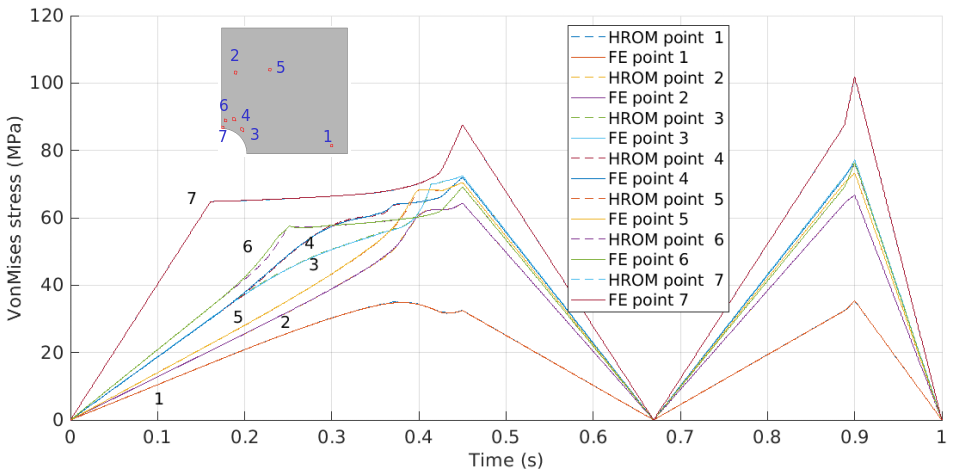
\includegraphics[width=0.8\textwidth]{FIGS/stress_vm.png}
\caption{Evolution of the von Mises equivalent stress  during the generalization test at the seven
Gauss points selected by MAW--ECM.
   The inset identifies the
location and numbering of the selected points.}
\label{fig:damage_maw_local_stresses}
\end{figure}


 Finally, Figure~\ref{fig:damage_maw_local_stresses} compares the von
Mises stress histories predicted by the FE model and the adaptive
manifold HROM at the seven selected Gauss points along the
generalization trajectory.  With the
exception of a small discrepancy at point \(6\) during the initial
damage transition, approximately over
\(0.2\lesssim t\lesssim0.3\),  the FE and manifold-HROM stress histories practically coincide.  The agreement is maintained not only
during the tensile branch represented in the training data, but also
throughout unloading, reverse loading in compression, and the final
return to the unloaded state.  Particularly noteworthy is point \(7\),
located in the vicinity of the hole and subjected to the largest stress
concentration.  Despite exhibiting the highest stresses and the
largest variation over the cycle, its complete history is reproduced
at plotting resolution.





\section{Concluding remarks}
\PROMPT{\input{Prompt_conclusions}}
%\input{Conclusions_1}
%\input{Conclusions_2}

This work has explored the use of state-dependent integration weights
for the hyperreduction of nonlinear-manifold reduced-order models.
The underlying idea is admittedly simple, but constitutes a significant
departure from the usual ECM/ECSW paradigm: the spatial support of the
cubature rule is kept fixed, while its positive weights are allowed to
vary with the position on the solution manifold. The resulting
MAW--ECM formulation, introduced in Section~\ref{sec:MAWECM}, may thus
be regarded as an attempt to make the integration rule conform to the
same low-dimensional structure exploited by the nonlinear kinematic
representation.

The numerical evidence obtained from the two benchmarks supports this
idea. A fixed-weight ECM rule is constructed from a global linear
approximation of the sampled integrands and must therefore accommodate
their complete retained linear span. MAW--ECM, by contrast, imposes
integration conditions locally at the sampled manifold states. In this
sense, it seeks to integrate the family of integrands actually visited
by the reduced model, rather than the larger linear space generated by
them. This distinction appears to be the main reason behind the
additional sparsity obtained with adaptive weights.

In the hyperelastic metamaterial of
Section~\ref{sec:metamaterial}, the nonlinear manifold already provides
a substantial reduction, both in kinematic dimension and in the size of
the corresponding fixed cubature rule. Starting from the latter,
MAW--ECM removes approximately \(80\%\) of the remaining integration
points, while preserving essentially the same level of displacement
accuracy and maintaining a small error in the homogenized stresses.
The results also confirm the role of graph regularization: smoothness
of the sampled weight fields is not merely an aesthetic requirement,
but has a direct influence on the quality of their subsequent
regression and, consequently, on the online response.

The effect is considerably stronger in the continuum-damage problem of
Section~\ref{sec:DamageProblem}. There, MAW--ECM eliminates more than
\(97\%\) of the points of the fixed-weight manifold rule, leaving only
a very small common support. This suggests that adaptive weights may be
particularly advantageous in propagation-dominated problems. Damage
produces an evolving localized nonlinear region, and a fixed cubature
rule must retain enough spatial information to represent its different
positions throughout the loading history. Adaptive weights can instead
redistribute the relative importance of a much smaller set of retained
points as the nonlinear region evolves. In this sense, the pruning
procedure appears to identify automatically the regions carrying the
most relevant mechanical information, leaving a sparse set of
integration points that may be viewed, metaphorically, as structural
``sensors''.

The damage benchmark also provides a demanding generalization test.
The reduced models were trained exclusively on a monotonic tensile
trajectory, whereas the testing history includes unloading, reverse
loading in compression, and final unloading. Nevertheless, the
adaptive manifold HROM reproduces not only the global displacement and
stress--strain response, but also the local stress histories at the
retained integration points. This agreement is particularly noteworthy
because these local histories are not prescribed by the cubature
construction itself; rather, they emerge from the solution of the
hyperreduced equilibrium equations together with the constitutive
updates performed at the selected points.

A second conclusion concerns the construction of the nonlinear
manifolds. In the two examples considered here, maximum kinematic
compression was sought by allowing the latent coordinates to be general
linear combinations of the retained modal amplitudes. The particular
identification procedures were purposely tailored to each benchmark.
For the metamaterial, the geometry of the sampled solution manifold was
sufficient to identify an appropriate two-dimensional parametrization.
For the history-dependent problem, by contrast, physical knowledge of
the constitutive response proved essential: exploiting the invariance
associated with elastic unloading made it possible to separate the
reversible dependence on load amplitude from the irreversible evolution
of damage and reduce the nonlinear closure to a univariate regression.
Interestingly, the resulting nonlinear latent coordinate subsequently
acquired the interpretation of a structural-scale counterpart of the
local damage-history variable.

These examples therefore illustrate complementary roles for data and
physical insight in manifold construction. The procedures adopted here
are admittedly problem-dependent and are not presented as a general
solution to manifold learning. Nevertheless, in the absence of robust
general-purpose methodologies for strongly history-dependent problems,
the incorporation of elementary mechanical information may considerably
reduce both the dimension of the learning problem and the amount of
training data required. By contrast, once a manifold representation has
been supplied, the MAW--ECM pruning procedure itself is essentially
automatic.

The present study should be regarded as exploratory. Both benchmarks
involve at most two latent coordinates, and extending the methodology
to substantially higher-dimensional manifolds remains an important
open question. Of particular concern is the graph-regularized
redistribution introduced in Section~\ref{sec:MAWECM}, whose global
coupling may become prohibitively expensive as the number of sampled
latent states increases. The numerical experiments are encouraging in
that regularization is required only during a relatively small fraction
of the pruning process, but more scalable alternatives---possibly based
on local graphs, partitions, or clusters of the latent space---should
be investigated.

Finally, extrapolation of the adaptive weight fields deserves specific
attention. Positivity is enforced at the sampled latent states, but is
not automatically guaranteed by a generic regression outside the
training domain. Constraint-preserving regressions constitute one
possible route. Another, particularly simple possibility would be to
enrich the regression dataset outside the high-fidelity training region
using inexpensive low-fidelity predictions provided by a fixed-weight
manifold HROM. These issues, together with the extension to
higher-dimensional latent spaces and more complex constitutive models,
define the natural next steps for assessing how far the proposed
adaptive-weight paradigm can be carried.

\section*{Acknowledgements}

Joaquín A. Hernández and S. Ares de Parga acknowledge  the support of Grant PID2024-158878OB-C21 funded by MICIU/AEI /10.13039/501100011033 and by ERDF/EU.


\appendix
 \section{Consistent linearization of the MAW--ECM equilibrium equations}
\label{app:MAW_linearization}
%\input{Linear_1}


This appendix derives the consistent Newton--Raphson linearization of
the MAW--ECM reduced equilibrium equations introduced in
Eq.~\refeq{eq:MAW_ROM_equilibrium}. The residual depends on the latent
coordinates through the constitutive response, the manifold tangent
basis,  and additionally
through the adaptive cubature weights. The resulting tangent operator
therefore comprises the standard and manifold-curvature contributions,
together with a new term arising from the variation of the weight
fields.

For convenience, Eq.~\refeq{eq:MAW_ROM_equilibrium} is first recast in
residual form. Defining
\begin{equation}
\label{eq:MAW_online_residual}
\Rdec(\qM;\muvec)
\defeq
\sum_{g\in\Zomega}
\rDec{g}(\qM;\muvec)\,
\omegag{g}(\qM)
-
\FextD(\qM;\muvec),
\end{equation}
where \(\rDec{g}\) and \(\FextD\) are given by
Eqs.~\refeq{eq:rDec_definition} and~\refeq{eq:FextD}, respectively,
the reduced equilibrium equations read
\begin{equation}
\label{eq:MAW_online_equilibrium_residual}
\Rdec(\qM;\muvec)=\bm{0}.
\end{equation}
The consistent tangent matrix,
\(\KtanD\in\RRn{\rD}{\rD}\), is obtained by differentiating
Eq.~\refeq{eq:MAW_online_residual} with respect to the latent
coordinates. Using the factorized decoder introduced in
Eq.~\refeq{eq:decoder_tau_generic}, together with
Eqs.~\refeq{eq:PhiD_tau_generic} and~\refeq{eq:FextD}, the result can
be written as
\begin{equation}
\label{eq:manifold_tangent_split_maw}
\KtanD
=
\KstdD
+
\KcurvD
+
\KweigD .
\end{equation}
The three terms account, respectively, for the constitutive
linearization, the curvature of the approximation manifold, and the
variation of the adaptive cubature weights.

Let
\[
\KFEg{g}
:=
\frac{\partial\rFE{g}}{\partial\dred}
\]
denote the consistent Gauss-point tangent operator. The standard contribution
is
\begin{equation}
\label{eq:manifold_standard_tangent_maw}
\KstdD
=
\JTAU^T
\left(
\sum_{g\in\Zomega}
\PhiROM^T
\KFEg{g}
\PhiROM\,
\omegag{g}
\right)
\JTAU.
\end{equation}
The curvature contribution is expressed componentwise as
\begin{equation}
\label{eq:manifold_curvature_tangent_maw}
\left(\KcurvD\right)_{ab}
=
\left[
\frac{\partial^2\TAU}
{\partial q_{M,a}\,\partial q_{M,b}}
\right]^T
\RTauD,
\qquad
a,b=1,\ldots,\rD,
\end{equation}
where
\begin{equation}
\label{eq:residual_tau_maw}
\RTauD
:=
\sum_{g\in\Zomega}
\PhiROM^T
\rFE{g}\,
\omegag{g}
-
\FextONEtau\muvec .
\end{equation}
Notice that the residual in Eq.~\eqref{eq:MAW_online_residual}
satisfies
\begin{equation}
\label{eq:residual_factorization_maw}
\Rdec
=
\JTAU^T\RTauD.
\end{equation}
Finally, the dependence of the cubature weights on the latent
coordinates gives
\begin{equation}
\label{eq:KweightD_def}
\begin{aligned}
\KweigD
&=
\JTAU^T
\sum_{g\in\Zomega}
\left(
\PhiROM^T\rFE{g}
\right)
\frac{\partial\omegag{g}}{\partial\qM}
\\
&=
\sum_{g\in\Zomega}
\rDec{g}
\frac{\partial\omegag{g}}{\partial\qM}.
\end{aligned}
\end{equation}
Here,
\(\partial\omegag{g}/\partial\qM\in\mathbb{R}^{1\times\rD}\)
is obtained by differentiating the regression model used to represent
the corresponding weight field.

For a fixed-weight rule,
\(\partial\omegag{g}/\partial\qM=\bm{0}\), and therefore
\(\KweigD=\bm{0}\). Likewise, \(\KcurvD\) vanishes when the decoder is
affine (that is, when $\JTAU = \ident$).
% The consistent tangent matrix, denoted by $\KtanD \in \RRn{\rD}{\rD}$ is obtained by differentiating
% Eq.~\refeq{eq:MAW_online_residual} with respect to the latent
% coordinates. We begin by taking variations of such an equation:
% \begin{equation}
% \label{eq:MAW_residual_variation}
% \delta\Rdec
% =
% \sum_{g\in\Zomega}
% \delta\rDec{g}\,
% \omegag{g}
% +
% \sum_{g\in\Zomega}
% \rDec{g}\,
% \delta\omegag{g}
% -
% \delta\FextD .
% \end{equation}







 \bibliographystyle{plain}
\bibliography{Bibliography}

\end{document}
